% SPDX-FileCopyrightText: 2026 Mert Torun
% SPDX-License-Identifier: CC-BY-4.0

\documentclass[12pt, a4paper, oneside]{report}

% SPDX-FileCopyrightText: 2026 Mert Torun
% SPDX-License-Identifier: CC-BY-4.0

% --- Fonts & Encoding (LuaLaTeX / OpenType via fontspec) ---
% Body text : TeX Gyre Termes      (Times-compatible serif)
% Headings   : TeX Gyre Heros       (Helvetica-compatible sans)
% Monospace  : Inconsolata (zi4)    (matches the former zi4 package)
% Mathematics: TeX Gyre Termes Math (OpenType, pairs with the body serif)
% All four ship with TeX Live full, so the CI container needs no extra fonts.
\usepackage{fontspec}
\usepackage[english]{babel}
\usepackage{csquotes}
\usepackage{xcolor}
\usepackage{amsmath}
\usepackage{unicode-math}
\setmainfont{TeX Gyre Termes}
\setsansfont{TeX Gyre Heros}[Scale=0.90]
\setmonofont{Inconsolatazi4}[
    Extension   = .otf,
    UprightFont = *-Regular,
    BoldFont    = *-Bold,
    ItalicFont  = *-Regular,
    Scale       = 0.85
]
\setmathfont{TeX Gyre Termes Math}

% --- Layout & Typography ---
\usepackage{geometry}
\geometry{left=3cm, right=2.5cm, top=2.5cm, bottom=2.5cm}
\usepackage{setspace}
\onehalfspacing
\setlength{\emergencystretch}{3em}
\sloppy
\hbadness=10000
\vbadness=10000
\usepackage{microtype} % Improved typography spacing
\usepackage{fancyhdr}
\usepackage[absolute,overlay]{textpos}
\usepackage{multicol}
\usepackage{array}
\usepackage{tabularx}
\usepackage{siunitx}
\newcolumntype{L}[1]{>{\raggedright\arraybackslash}p{#1}}

% --- Graphics & Tables ---
\usepackage{graphicx}
\usepackage{float}
\usepackage{subcaption}
\usepackage{booktabs}
\usepackage{titlesec} 
\usepackage[nohyperlinks]{acronym}
\usepackage{tikz}
\usetikzlibrary{positioning,shapes,shapes.geometric,shapes.multipart,arrows,arrows.meta,calc,fit,backgrounds,chains,decorations.pathreplacing,decorations.markings}
\usepackage{listings}
\usepackage{upquote}
\usepackage[most]{tcolorbox} % Modern Boxes

% --- TH Koeln CI Colors ---
% Moved to setup/design.tex

% --- Modern Heading Styles ---
% Moved to setup/design.tex

% --- Bibliography (IEEE Style) ---
\usepackage[style=ieee, backend=biber]{biblatex}
\addbibresource{bibliography.bib}

% --- PDF Navigation ---
\usepackage[hidelinks, unicode, hypertexnames=false]{hyperref}

% SPDX-FileCopyrightText: 2026 Mert Torun
% SPDX-License-Identifier: CC-BY-4.0

% --- Thesis Metadata ---
\newcommand{\ThesisTitle}{Design and Implementation of a Modular Architecture for the Transparent Integration of Containerized Execution Environments for Heterogeneous Open-Source Binaries in OneWare Studio}
\newcommand{\ThesisAuthor}{Mert Torun}
\newcommand{\ThesisDate}{02.07.2026}

% --- Supervisors ---
\newcommand{\SupervisorA}{Prof. Dr. Tobias Krawutschke}
\newcommand{\SupervisorB}{M.Sc. Sebastian Wittlich}

% --- Institution ---
% The faculty of the M.Sc. programme, in TH Köln's own English wording;
% German: Fakultät für Informations-, Medien- und Elektrotechnik.
\newcommand{\University}{TH Köln -- University of Applied Sciences}
\newcommand{\Faculty}{Faculty of Information, Media and Electrical Engineering}


% Document information as the deposited file carries it (title, author,
% subject, keywords); setup/design sets only the colours of the links. The
% subject keeps the two hyphens of the deposited file: -{}- stops TeX from
% joining them into an en dash.
\hypersetup{
    pdftitle={\ThesisTitle},
    pdfauthor={\ThesisAuthor},
    pdfsubject={Master's Thesis, TH Köln -{}- University of Applied Sciences, 2026},
    pdfkeywords={FPGA Toolchains; Docker Middleware; Hybrid Strategy Pattern; Reproducible Builds; Cross-Platform Architecture; .NET 10; Apple Silicon Emulation; User-ID Mapping; Version Pinning; Electronic Design Automation (EDA); OneWare Studio}
}
% SPDX-FileCopyrightText: 2026 Mert Torun
% SPDX-License-Identifier: CC-BY-4.0

% --- TH Köln CI Colors ---
\definecolor{thred}{RGB}{204, 0, 0}
\definecolor{thorange}{RGB}{209, 65, 36}
\definecolor{thgray}{RGB}{75, 75, 75}
\definecolor{thlightgray}{RGB}{200, 200, 200}

% --- Logo Positioning & Graphics ---
\setlength{\TPHorizModule}{1mm}
\setlength{\TPVertModule}{1mm}

% --- Headings (Modern Sans-Serif) ---
\titleformat{\chapter}[display]
  {\normalfont\sffamily\huge\bfseries\color{thred}}
  {\chaptertitlename\ \thechapter}{20pt}{\Huge}
  [\vspace{1ex}\color{thgray}\titlerule] % Line below chapter title

\titleformat{\section}
  {\normalfont\sffamily\Large\bfseries\color{thgray}}
  {\thesection}{1em}{}

\titleformat{\subsection}
  {\normalfont\sffamily\large\bfseries\color{thgray}}
  {\thesubsection}{1em}{}

% --- Paragraphs ---
\setlength{\parindent}{0pt}
\setlength{\parskip}{0.5em}

% --- Header/Footer (FancyHdr) ---
\setlength{\headheight}{24.7pt} % Fix warning
\pagestyle{fancy}
\fancyhf{}
\fancyhead[R]{\thepage}
\fancyhead[L]{\sffamily\nouppercase{\leftmark}}
\renewcommand{\headrulewidth}{0.5pt}
\renewcommand{\headrule}{\hbox to\headwidth{\color{thred}\leaders\hrule height \headrulewidth\hfill}}

% --- Themed Hyperlinks ---
\hypersetup{
    colorlinks=true,
    linkcolor=thred,      % Internal links (TOC, figs) -> TH Red
    filecolor=thgray,
    urlcolor=thorange,    % URLs -> TH Orange
    citecolor=thorange    % Citations -> TH Orange
}

% --- Diagram House Style -----------------------------------------------------
% One shared vocabulary for every TikZ figure, so the diagrams are visually
% consistent. Text is set at a fixed document size in the sans face (TeX Gyre
% Heros) and is NEVER scaled with \resizebox, so diagram type matches the body
% and stays sharp. Colours reuse the TH palette defined above.
\tikzset{
    % Default arrow tip for every diagram.
    >={Stealth[length=2.2mm,width=1.7mm]},
    %--- Generic blocks ------------------------------------------------------
    fwbox/.style      = {draw=thgray, fill=thgray!6, rounded corners=2pt, align=center,
                         inner sep=4pt, minimum height=8mm, minimum width=28mm,
                         font=\footnotesize\sffamily, line width=0.6pt},
    fwstart/.style    = {fwbox, draw=thred, fill=thred!10, font=\footnotesize\sffamily\bfseries},
    fwaccent/.style   = {fwbox, draw=thred, fill=thred!8},
    fwalt/.style      = {fwbox, draw=thorange, fill=thorange!10},
    fwdecision/.style = {draw=thorange, fill=thorange!12, diamond, aspect=2.3, align=center,
                         inner sep=1pt, minimum height=8mm, font=\footnotesize\sffamily, line width=0.6pt},
    fwstate/.style    = {fwbox, minimum width=24mm},
    fwsystem/.style   = {draw=thgray, densely dashed, rounded corners=3pt, fill=thgray!3, inner sep=6pt},
    fwbranch/.style   = {draw=thgray, densely dashed, fill=thgray!4, rounded corners=2pt, align=left,
                         inner sep=4pt, text width=44mm, font=\scriptsize\sffamily, line width=0.6pt},
    %--- UML class (title compartment + member compartment) ------------------
    fwclass/.style    = {draw=thgray, fill=thgray!5, rounded corners=2pt, rectangle split,
                         rectangle split parts=2, align=left, inner sep=4pt, text width=50mm,
                         font=\footnotesize\sffamily, line width=0.6pt},
    fwinterface/.style= {fwclass, draw=thred, fill=thred!8},
    %--- Byte-layout cells ---------------------------------------------------
    fwcell/.style     = {draw=thgray, fill=thgray!6, minimum height=11mm, minimum width=15mm,
                         align=center, font=\scriptsize\sffamily, line width=0.6pt},
    fwcellhl/.style   = {fwcell, draw=thred, fill=thred!10},
    fwcellalt/.style  = {fwcell, draw=thorange, fill=thorange!10},
    %--- Sequence-diagram vocabulary ----------------------------------------
    fwactor/.style    = {draw=thgray, fill=thgray!8, rounded corners=2pt, align=center,
                         minimum height=7mm, minimum width=22mm, font=\scriptsize\sffamily\bfseries},
    fwlifeline/.style = {draw=thgray, densely dashed, line width=0.5pt},
    fwactivation/.style = {draw=thgray, fill=thgray!15, minimum width=2.2mm},
    %--- Edges ---------------------------------------------------------------
    fwedge/.style     = {->, draw=thgray, line width=0.6pt},
    fwedgehl/.style   = {fwedge, draw=thred},
    fwedgealt/.style  = {fwedge, draw=thorange},
    fwdep/.style      = {->, draw=thorange, densely dashed, line width=0.6pt},
    fwrealize/.style  = {-{Triangle[open, length=2.8mm, width=2.8mm]}, draw=thgray, densely dashed, line width=0.6pt},
    fwmsg/.style      = {-{Stealth[length=2mm]}, draw=thgray, line width=0.5pt, font=\scriptsize\sffamily},
    fwreturn/.style   = {-{Stealth[length=2mm]}, draw=thgray, densely dashed, line width=0.5pt, font=\scriptsize\sffamily},
    %--- Edge label chip (white backing so labels never collide with lines) --
    fwlabel/.style    = {font=\scriptsize\sffamily, fill=white, inner sep=1.5pt},
}
 % Modern Design
% SPDX-FileCopyrightText: 2026 Mert Torun
% SPDX-License-Identifier: CC-BY-4.0

% --- Modern Light Editor Colors ---
\definecolor{codecomment}{RGB}{0, 128, 0}      % Forest Green
\definecolor{codekeyword}{RGB}{0, 102, 204}    % VS-like Blue
\definecolor{codestring}{RGB}{163, 21, 21}     % VS-like Dark Red
\definecolor{codetype}{RGB}{43, 145, 175}      % VS-like Teal
\definecolor{codebg}{RGB}{248, 249, 250}       % Soft Light-Gray
\definecolor{vsframe}{RGB}{220, 220, 220}      % Gray border
\definecolor{backcolour}{rgb}{0.96, 0.96, 0.97} 

% --- TColorBox Wrap ---
\tcbset{
    enhanced,
    colback=backcolour,
    boxrule=0.5pt,
    colframe=thgray!50,
    sharp corners,
    drop shadow={opacity=0.2}
}

% --- Listings Language Definitions ---

% CSharp Custom Definition
\lstdefinelanguage{CSharp}{
  sensitive=true,
  morekeywords=[1]{
    abstract, as, base, bool, break, byte, case, catch, char, checked,
    class, const, continue, decimal, default, delegate, do, double, else,
    enum, event, explicit, extern, false, finally, fixed, float, for,
    foreach, goto, if, implicit, in, int, interface, internal, is, lock,
    long, namespace, new, null, object, operator, out, override, params,
    private, protected, public, readonly, ref, return, sbyte, sealed,
    short, sizeof, stackalloc, static, string, struct, switch, this, throw,
    true, try, typeof, uint, ulong, unchecked, unsafe, ushort, using,
    virtual, void, volatile, while, add, alias, ascending, async, await,
    by, descending, dynamic, equals, from, get, global, group, into, join,
    let, on, orderby, partial, remove, select, set, value, var, where, yield
  },
  morekeywords=[2]{DockerService, ContainerExecutionAdapter, IToolExecutionStrategy, ToolCommand, IToolchainService, NativeService, ToolchainParser},
  morecomment=[l]{//},
  morecomment=[s]{/*}{*/},
  morestring=[b]",
  morestring=[b]',
}
\lstalias{csharp}{CSharp}

% JSON Custom Definition
\lstdefinelanguage{json}{
    basicstyle=\ttfamily\footnotesize,
    numbers=left,
    numberstyle=\tiny\sffamily\color{black},
    stepnumber=1,
    numbersep=12pt,
    showstringspaces=false,
    breaklines=true,
    frame=none,
    backgroundcolor=\color{codebg},
    xleftmargin=32pt,
    columns=fullflexible,
    keepspaces=true,
    string=[b]",
    stringstyle=\color{codestring},
    literate=
     *{0}{{{\color{blue}0}}}{1}
      {1}{{{\color{blue}1}}}{1}
      {2}{{{\color{blue}2}}}{1}
      {3}{{{\color{blue}3}}}{1}
      {4}{{{\color{blue}4}}}{1}
      {5}{{{\color{blue}5}}}{1}
      {6}{{{\color{blue}6}}}{1}
      {7}{{{\color{blue}7}}}{1}
      {8}{{{\color{blue}8}}}{1}
      {9}{{{\color{blue}9}}}{1}
      {:}{{{\color{punct}{:}}}}{1}
      {,}{{{\color{punct}{,}}}}{1}
      {\{}{{{\color{delim}{\{}}}}{1}
      {\}}{{{\color{delim}{\}}}}}{1}
      {[}{{{\color{delim}{[}}}}{1}
      {]}{{{\color{delim}{]}}}}{1},
}
\colorlet{punct}{red!60!black}
\definecolor{delim}{RGB}{20,105,176}

% --- Code Listing Style (In-Text Listings) ---
\lstdefinestyle{csharp-ci}{
    language=CSharp,
    backgroundcolor=\color{codebg},
    basicstyle=\ttfamily\footnotesize,
    breaklines=true,
    breakatwhitespace=true,
    captionpos=t,
    frame=none,
    xleftmargin=32pt,
    numbers=left,
    numbersep=12pt,
    numberstyle=\tiny\sffamily\color{black},
    columns=flexible,
    keepspaces=true,
    tabsize=4,
    showstringspaces=false,
    commentstyle=\color{codecomment},
    keywordstyle=\color{codekeyword}\bfseries,
    stringstyle=\color{codestring},
    keywordstyle=[2]\color{codetype}\bfseries,
    morekeywords={var, async, await, record, init, with, GeneratedRegex},
    morestring=[b]",
    morestring=[b]',
    literate={<}{{\textless}}1 {>}{{\textgreater}}1 {`}{{\char96}}1 {' '}{{{\textquotesingle\ \textquotesingle}}}3,
}

% --- Code Listing Style (Appendix Full-File Listings) ---
\lstdefinestyle{csharp-appendix}{
    language=CSharp,
    backgroundcolor=\color{codebg},
    basicstyle=\ttfamily\scriptsize,
    breaklines=true,
    breakatwhitespace=false,
    captionpos=t,
    frame=none,
    xleftmargin=32pt,
    numbers=left,
    numbersep=12pt,
    numberstyle=\tiny\sffamily\color{thgray},
    columns=flexible,
    keepspaces=true,
    tabsize=2,
    showstringspaces=false,
    commentstyle=\color{codecomment},
    keywordstyle=\color{codekeyword}\bfseries,
    stringstyle=\color{codestring},
    keywordstyle=[2]\color{codetype}\bfseries,
    morekeywords={var, async, await, record, init, with, GeneratedRegex},
    morestring=[b]",
    morestring=[b]',
    breakindent=6pt,
    postbreak=\raisebox{0ex}[0ex][0ex]{\ensuremath{\hookrightarrow\space}},
    literate={<}{{\textless}}1 {>}{{\textgreater}}1 {`}{{\char96}}1 {' '}{{{\textquotesingle\ \textquotesingle}}}3,
}

\lstset{style=csharp-ci}


\begin{document}

\pagenumbering{roman}
\pagestyle{plain}
% SPDX-FileCopyrightText: 2026 Mert Torun
% SPDX-License-Identifier: CC-BY-4.0

\begin{titlepage}
    % Vertical Branding Bar
    \begin{tikzpicture}[remember picture,overlay]
        \fill[thred] (current page.north west) rectangle ([xshift=2cm]current page.south west);
    \end{tikzpicture}

    % Logo Top Right (Absolute Positioning)
    \begin{textblock}{50}(150,10) 
        
\includegraphics[width=50mm]{figures/th_logo}
    \end{textblock}
    \vspace{3cm}

    % Left Aligned Content ("1.0 Grade" Modern Look)
    \begin{flushleft}
        \sffamily
        
        \vspace{1cm}
        {\large \scshape Master Thesis \par}
        \vspace{0.5cm}
        
        % Title with TH-Red Accent
        {\Huge \bfseries \color{thred} \ThesisTitle \par}
        \vspace{2cm}

        {\Large \textbf{\ThesisAuthor} \par}

        \vfill
        
        % Metadata Block
        \textbf{Institution:}\\ \University\\ \Faculty \\[1em]
        \textbf{Date:} \ThesisDate \\[1em]
        \textbf{Supervisors:}\\ \SupervisorA\\ \SupervisorB
    \end{flushleft}
\end{titlepage}

\clearpage

% SPDX-FileCopyrightText: 2026 Mert Torun
% SPDX-License-Identifier: CC-BY-4.0

\chapter*{Declaration on the Use of Aids}
\thispagestyle{empty}

The statutory declaration (\textit{Eidesstattliche Erklärung}) for this thesis is provided on the official cover sheet (\textit{Deckblatt}). For transparency, I declare here the aids used in its preparation: in addition to the cited sources and standard software, I used AI-based assistance for language editing, formatting, and reviewing the manuscript. The design, implementation, evaluation, and all conclusions are my own; every part was authored, checked, and verified by me, and I take full responsibility for the correctness of the content.

\clearpage

% SPDX-FileCopyrightText: 2026 Mert Torun
% SPDX-License-Identifier: CC-BY-4.0

\chapter*{Abstract}

Ensuring the reproducibility of build processes poses a significant challenge in embedded systems and Field-Programmable Gate Array (FPGA) development. The reliance on complex, platform-specific binaries and toolchains (e.g., Yosys, nextpnr) frequently leads to ``Environment Drift,'' where builds succeed locally but fail in collaborative environments due to system inconsistencies.

To address these challenges, this thesis investigates three central Research Questions: how to establish a robust, cross-platform containerization architecture across heterogeneous host operating systems (RQ1), how to seamlessly integrate these containerized environments into a modern IDE to preserve a native user experience (RQ2), and what performance overhead is introduced by containerized execution and architecture emulation (RQ3). To resolve these questions, a modular software integration architecture is designed and implemented as a standalone extension for the \textit{OneWare Studio} IDE. Using C\# and .NET 10, a decoupled middleware is developed based on a \textbf{Hybrid Strategy Pattern}, enabling developers to switch seamlessly between high-performance native execution and hermetic containerized workflows at runtime.

The architecture resolves critical barriers to adoption through four technical contributions---three addressing the research questions directly, complemented by a reproducibility feature:
\begin{enumerate}
    \item \textbf{Cross-Platform Interoperability (Addressing RQ1):} A dynamic User-ID injection strategy and abstract transport resolution ensure seamless operation across Windows, Linux, and macOS, specifically solving file-permission locking issues on Linux systems.
    \item \textbf{Transparent Integration (Addressing RQ2):} Real-time stream multiplexing and log-level parsing transform raw container output into structured IDE feedback, preserving the native user experience.
    \item \textbf{Performance Characterization (Addressing RQ3):} The system exposes a user-selectable image platform so that, on ARM64 Apple Silicon, an x86 toolchain image is executed through the host runtime's Rosetta~2 translation layer; the resulting execution overhead is characterized and decomposed.
    \item \textbf{Temporal Reproducibility (``Time Machine''):} A dynamic tagging mechanism lets projects pin a specific toolchain image tag (optionally a content digest), providing a reproducible build environment over time.
\end{enumerate}

The empirical evaluation characterizes the cost of the containerized path rather than asserting a single headline factor. Beyond raw containerization, the extension's strategy dispatch adds a fixed per-invocation cost on the order of \SI{0.2}{\second} and negligible marginal compute overhead, so its relative cost is dominated by a constant floor that amortizes as workload size grows. On Apple Silicon the toolchain image runs under Rosetta~2 emulation, so a native-versus-container comparison on that host would conflate containerization with instruction-set emulation; native \texttt{x86\_64} hosts (Windows and Linux) reproduce the same fixed-floor structure without emulation, and the same-build native baseline on the Linux host---the one setting that isolates the container-versus-native factor---fixes it at $\alpha \approx 1$, a fixed per-invocation floor with no measurable per-instruction tax. Across the seven-workload FPGA corpus (iCE40 and ECP5 synthesis, place-and-route and bitstream packing, plus Icarus~Verilog simulation) every workload executed to success through the hermetic container, so the system eliminates configuration friction and makes toolchain execution independent of the host's package environment, resolving cascading dependency conflicts.

\clearpage


% SPDX-FileCopyrightText: 2026 Mert Torun
% SPDX-License-Identifier: CC-BY-4.0

\vspace{1cm}
\textbf{Keywords:} FPGA Toolchains; Docker Middleware; Hybrid Strategy Pattern; Reproducible Builds; Cross-Platform Architecture; .NET 10; Apple Silicon Emulation; User-ID Mapping; Version Pinning; Electronic Design Automation (EDA); OneWare Studio.

\clearpage

\tableofcontents
\clearpage

\listoffigures
\clearpage

\listoftables
\clearpage

\lstlistoflistings
\clearpage

% SPDX-FileCopyrightText: 2026 Mert Torun
% SPDX-License-Identifier: CC-BY-4.0

\chapter*{List of Acronyms}

\begin{acronym}[FPGA]
    \acro{AOT}{Ahead-of-Time (Compilation)}
    \acro{API}{Application Programming Interface}
    \acro{CI}{Continuous Integration}
    \acro{CLI}{Command Line Interface}
    \acro{CLR}{Common Language Runtime}
    \acro{CPU}{Central Processing Unit}
    \acro{DAX}{Direct Access}
    \acro{DBT}{Dynamic Binary Translation}
    \acro{EDA}{Electronic Design Automation}
    \acro{FPGA}{Field-Programmable Gate Array}
    \acro{GID}{Group Identifier}
    \acro{GUI}{Graphical User Interface}
    \acro{HDL}{Hardware Description Language}
    \acro{I/O}{Input/Output}
    \acro{IDE}{Integrated Development Environment}
    \acro{IPC}{Inter-Process Communication}
    \acro{ISA}{Instruction Set Architecture}
    \acro{JIT}{Just-in-Time (Compilation)}
    \acro{OCI}{Open Container Initiative}
    \acro{OOM}{Out of Memory}
    \acro{OS}{Operating System}
    \acro{RISC}{Reduced Instruction Set Computer}
    \acro{RTL}{Register-Transfer Level}
    \acro{TSO}{Total Store Ordering}
    \acro{UID}{User Identifier}
    \acro{UX}{User Experience}
    \acro{VHDL}{VHSIC Hardware Description Language}
    \acro{VM}{Virtual Machine}
    \acro{WMO}{Weak Memory Ordering}
    \acro{WSL2}{Windows Subsystem for Linux~2}
\end{acronym}

\clearpage

\clearpage
\pagenumbering{arabic}
\pagestyle{fancy}

% SPDX-FileCopyrightText: 2026 Mert Torun
% SPDX-License-Identifier: CC-BY-4.0

\chapter{Introduction}
\label{ch:introduction}

The development of embedded systems and Field-Programmable Gate Arrays (FPGAs) has evolved significantly over the past decade. Modern hardware designs typically rely on extensive, often open-source toolchains---such as \textit{Yosys} for synthesis~\cite{wolf2013yosys}, \textit{nextpnr} for place-and-route~\cite{shah2019nextpnr}, and \textit{Verilator}~\cite{snyder2004verilator} and \textit{Icarus~Verilog} for simulation. While these tools offer powerful capabilities, ensuring the reproducibility of build processes across heterogeneous development environments remains a critical challenge in Electronic Design Automation (EDA).

\section{Motivation and Problem Context}
In collaborative projects, a phenomenon widely referred to as ``Environment Drift'' poses a significant barrier to efficiency. A build process that succeeds on a developer's local machine frequently fails on a colleague's workstation or the Continuous Integration (CI) server due to subtle differences in system libraries, binary versions, or path configurations~\cite{courtes2013functional}.

In the specific context of \textit{OneWare Studio}, an Integrated Development Environment (IDE) aiming to unify FPGA development, the reliance on locally installed toolchains presents a bottleneck. Users are currently required to manually install and configure complex binaries that vary significantly between operating systems (Windows 11, macOS Tahoe 26.6, Ubuntu 26.04).

\section{Problem Statement}
Containerization technologies (e.g., Docker) offer a potential solution by encapsulating build tools into immutable artifacts (``Hermetic Builds''). However, standard Docker workflows typically require interaction via the Command Line Interface (CLI), which disrupts the seamless user experience expected from a GUI-based IDE. Specifically, three technical challenges inhibit widespread adoption:

\begin{enumerate}
    \item \textbf{System Heterogeneity (RQ1):} The diversity of host platforms creates a compatibility matrix that is difficult to maintain natively. Integrating Docker requires handling platform-specific constraints, such as the divergence between Named Pipes on Windows and Unix Domain Sockets on Linux/macOS. Additionally, Linux file permissions often cause artifacts to be locked by the \texttt{root} user.
    \item \textbf{Integration Gap (RQ2):} Developers must currently switch contexts between the IDE and a terminal to run container commands, breaking the ``Flow'' state. Real-time feedback, such as streamed build output in the IDE console, is lost.
    \item \textbf{Performance Overhead (RQ3):} On Apple Silicon (ARM64), running the reference toolchain image---published for \texttt{x86\_64} (\texttt{linux/amd64}) only---creates an instruction-set mismatch with the host. Executing it through the runtime's Rosetta~2 translation layer introduces a performance penalty that must be quantified to justify the trade-off.
\end{enumerate}

\section{Research Objectives}
To address the described problem statement, this thesis follows a structured approach ranging from architectural design to user-experience validation. The research is guided by the following three research questions, ordered to mirror the development lifecycle. RQ1 and RQ3 are assessed quantitatively in the evaluation---for RQ3, the marginal cost of the integration layer is measured directly on all three hosts, the emulated-regime penalty is cited from the literature, and the native-versus-container factor is isolated only on a host with a same-build native baseline and is measured on the Linux host, the only one of the three that admits such a baseline (Machine~2). RQ2, concerned with the transparency and feel of the integration, is assessed qualitatively against the implemented behavior:

\begin{itemize}
    \item \textbf{RQ1 (Architectural Foundation):} What architectural patterns ensure cross-platform compatibility for container orchestration across Windows, Linux, and macOS, specifically addressing low-level challenges like User-ID mapping and transport protocols?
    \item \textbf{RQ2 (Transparent Integration):} How can these containerized environments be integrated into a .NET-based IDE to provide a ``Native User Experience,'' preserving essential features like real-time streamed log feedback and structured diagnostics?
    \item \textbf{RQ3 (Performance Viability):} What is the measurable performance overhead of this containerized approach compared to native execution, particularly when bridging architecture gaps (x86 on ARM64)?
\end{itemize}

\section{Structure of the Thesis}
The remainder of this thesis is organized as follows. Chapter~\ref{ch:background} establishes the theoretical foundations of containerization, virtualization, and cross-architecture execution. Chapter~\ref{ch:stateoftheart} surveys the state of the art in reproducible EDA tooling and positions this work against existing approaches. Chapter~\ref{ch:concept} presents the modular architecture---the hybrid execution strategy, transport resolution, and container lifecycle---which Chapter~\ref{ch:implementation} then realizes in detail. Chapter~\ref{ch:evaluation} reports the empirical evaluation of the integration overhead and cross-platform output determinism across the test machines, and Chapter~\ref{ch:conclusion} summarizes the contributions and outlines directions for future work.

% SPDX-FileCopyrightText: 2026 Mert Torun
% SPDX-License-Identifier: CC-BY-4.0

\chapter{Theoretical Background}
\label{ch:background}

This chapter establishes the fundamental concepts and technologies required for the design of the containerized integration architecture. It provides a detailed analysis of virtualization paradigms, the internal mechanisms of the Docker engine, and the specific requirements of modern FPGA design flows.

\section{Virtualization Paradigms in Software Engineering}
Virtualization is the abstraction of computing resources to create isolated execution environments. In the context of this thesis, two primary paradigms are relevant: Hardware Virtualization (Hypervisors) and Operating System-level Virtualization (Containers)~\cite{felter2015performance}. The choice between these paradigms determines the execution overhead, startup latency, and isolation characteristics of the compilation environment.

To quantitatively contrast these paradigms, Table~\ref{tab:virtualization_paradigms} lists the key architectural properties and associated latency costs.

\begin{table}[H]
    \caption{Comparative Analysis of Virtualization Paradigms and System Latency}
    \label{tab:virtualization_paradigms}
    \centering
    \begin{tabularx}{\textwidth}{@{} >{\raggedright\arraybackslash}p{4.0cm} X X @{}}
    \toprule
    \textbf{Architectural Metric} & \textbf{Hardware Virtualization (VM)} & \textbf{OS-level Virtualization (Container)} \\
    \midrule
    \textbf{CPU State Transition} & Hypervisor Trap / VM-Exit ($\approx \num{1000}\text{--}\num{3000}$ CPU cycles) & Native Syscall Trap ($\approx \num{100}\text{--}\num{300}$ CPU cycles) \\
    \textbf{Page Table Translation} & Two-Dimensional Paging (EPT/SLAT) & Native MMU Page Table Translation \\
    \textbf{Kernel Instances} & Isolated Guest Kernel per VM & Shared Host Kernel \\
    \textbf{Memory Allocation} & Statically Partitioned / Pre-allocated & Dynamically Allocated via Host \\
    \textbf{Storage I/O Overhead} & Block-level Emulation / Virtual Disk & UnionFS / Native Bind Mounts \\
    \textbf{Typical Boot Time} & Seconds to Minutes (\SIrange{10}{60}{\second}) & Milliseconds (\SIrange{50}{200}{\milli\second}) \\
    \bottomrule
    \multicolumn{3}{@{}>{\scriptsize}p{\dimexpr\textwidth\relax}@{}}{Cycle and latency figures are representative order-of-magnitude values;~\cite{felter2015performance} provides an application-level container-versus-VM performance comparison.}
    \end{tabularx}
\end{table}

\subsection{Hardware Virtualization (Hypervisors)}
Hardware virtualization, managed by a Hypervisor (Type 1 running directly on bare metal, or Type 2 running on a host OS), creates fully isolated Virtual Machines (VMs).
The guest operating system executes instruction streams within a deprivileged processor execution mode (e.g., Intel VMX non-root operation). Non-virtualizable sensitive instructions trigger a \textit{VM-exit} event, forcing a context switch back to the host hypervisor for software emulation. 

On macOS, the native kernel virtualization is exposed via the low-level \texttt{Hypervisor.framework} (which provides APIs for direct interaction with CPU virtualization features like VT-x/Intel VMX or Apple Silicon ARMv8 virtualization extensions) and the higher-level \texttt{Virtualization.framework} (which abstracts the bootloaders, virtual devices, and VM configuration). On Apple Silicon hosts, virtualization introduces unique scheduling dynamics. The host OS must map guest vCPU threads onto the physical asymmetrical cores: high-frequency Performance (P) cores and energy-efficient Efficiency (E) cores. The macOS thread scheduler manages these guest vCPU threads dynamically, but CPU pinning (affinity) is not natively supported by the framework. If guest threads are scheduled onto E-cores during intensive FPGA compilation, performance degrades significantly. Additionally, VM-exit penalties on ARM64 are caused by hypervisor traps for virtual timer access, interrupt handling, or generic stage-2 translation faults. While hardware-assisted translation (Two-Level Address Translation or Stage 2 Translation in ARMv8) reduces MMU translation latency by caching Guest Physical to Host Physical mappings in the TLB, TLB misses require walking two independent sets of page tables, incurring a measurable performance tax on translation-heavy workloads compared to native execution.

Memory management in VMs introduces significant overhead due to Second Level Address Translation (SLAT), implemented as Extended Page Tables (EPT) on Intel CPUs or Nested Page Tables (NPT) on AMD CPUs. When the guest OS translates a guest virtual address to a guest physical address, the MMU must walk the two-dimensional guest-to-host page tables. This can double the page table walk latency in the worst-case cache-miss scenarios. Storage \text{I/O} similarly suffers from an emulation tax, where block device requests pass through multiple layers of virtualized queue adapters before reaching host storage. These factors result in a high resource overhead and make hypervisors unsuitable for the rapid, low-latency, iterative compile-and-run cycles required by modern Integrated Development Environments (IDEs).

\subsection{Operating System-level Virtualization (Containers)}
OS-level virtualization creates isolated user-space instances (containers) that share the host operating system's kernel. Rather than emulating hardware, it relies on host kernel features to partition resources, allowing processes inside the container to execute at native hardware speeds. System calls pass directly to the host kernel with normal kernel trap latencies, avoiding the VM-exit penalty. 

For EDA toolchains, OS-level virtualization enables the concept of \textit{Hermetic Builds}: environments that are completely self-contained and reproducible across developer machines. By locking the exact tool versions and system shared library hashes within an immutable container image, the container-based approach mitigates environmental divergence without incurring detrimental performance latency.

\subsection{Open Container Initiative (OCI) Standards}
To prevent vendor lock-in and ensure interoperability, modern containerization is governed by the Open Container Initiative (OCI) standards. The OCI Image Specification establishes a strict, content-addressable design~\cite{oci2017image}. An image is structured as a collection of tar files representing filesystem layers, coupled with a JSON manifest and a JSON configuration file.
Content Addressability is achieved using cryptographic hashing (SHA-256). Every layer tarball, configuration file, and manifest is stored and indexed by its hash value. This allows the container engine to verify image integrity and reuse existing layers across different images, saving storage space and download bandwidth.
The image manifest---itself a content-addressed JSON blob rather than a fixed filename---links these components together by listing the digests of the filesystem layers and the image configuration. The configuration file specifies execution metadata (environment variables, entrypoints, user accounts, and CPU architecture).
During runtime instantiation, the engine (e.g., \texttt{containerd}) downloads and verifies these layers. It then stacks them using a union filesystem like OverlayFS, presenting a unified read-only directory structure (the rootfs) to the runtime execution tool (e.g., \texttt{runc}).

The OCI Runtime Specification governs the execution environment~\cite{oci2017runtime}. The engine creates an isolated container environment using host kernel namespaces and cgroups as configured in the runtime's configuration file (\texttt{config.json}). The runtime defines standard lifecycle operations:
\begin{enumerate}
    \item \textbf{create:} The container environment is created, namespaces are set up, and the init process is suspended before executing the entrypoint.
    \item \textbf{start:} The suspended process is resumed, starting the target program.
    \item \textbf{kill:} Sends a signal to the container processes.
    \item \textbf{delete:} Cleans up the namespaces and resource limits.
\end{enumerate}
The standardized OCI APIs allow container engines (such as Docker, Podman, or containerd) to swap underlying runtimes transparently, facilitating consistent execution environments across Linux, Windows, and macOS hosts.

\section{The Docker Container Engine}
Docker is the de-facto standard implementation of OS-level virtualization. It operates as a daemon (\texttt{dockerd}) that exposes a RESTful socket API to manage images, networks, volumes, and containers. The underlying container execution is driven by low-level kernel primitives, ensuring that containers run isolated processes with native scheduling and negligible hardware abstraction overhead.

\subsection{Kernel Namespaces}
Namespaces provide process-level resource isolation, partitioning the kernel resources so that a group of processes sees one set of resources while another group sees another.
\begin{enumerate}
    \item \textbf{PID Namespace:} Virtualizes process IDs, meaning the first process spawned inside the container becomes PID 1. This prevents containerized processes from viewing or signaling processes on the host or other containers.
    \item \textbf{Mount Namespace (mnt):} Isolates filesystem mount points. The container sees a custom directory layout with its own root directory (\texttt{/}) independent of the host. Crucially, mount propagation flags control how mounts inside or outside the namespace affect each other:
    \begin{itemize}
        \item \textbf{shared:} Mounts propagate in both directions. A mount inside the container propagates to the host, and vice versa.
        \item \textbf{slave:} Mounts propagate only from the host to the container. If the host mounts a new volume under a shared mount, the container sees it, but mounts created inside the container do not reflect back on the host.
        \item \textbf{private:} Mounts do not propagate in either direction. The containerized mount environment is completely decoupled from the host.
        \item \textbf{rprivate/rshared/rslave:} Recursive versions of the above flags, which apply the propagation properties to all sub-mounts within the directory tree. Docker bind mounts default to \texttt{rprivate} (recursive-private, no propagation in either direction). Correct propagation settings are critical for mounting active design workspaces, preventing host-level modifications from breaking container compiler contexts.
    \end{itemize}
    \item \textbf{User Namespace (user):} Maps user and group IDs (UID/GID) inside the container to a different set of IDs on the host. This is a critical security feature: a process running as root (UID~0) inside the container can be mapped to an unprivileged user (e.g., UID~10001) on the host, preventing host takeover if a container breakout occurs.
    
    In modern rootless container architectures, user namespaces enable unprivileged users to create and run containers safely without requiring root access on the host operating system~\cite{Lin2018ContainerSecurity}. When an unprivileged user starts a rootless container, the container engine uses helper binaries like \texttt{newuidmap} and \texttt{newgidmap} to consult the host's configuration files, namely \texttt{/etc/subuid} and \texttt{/etc/subgid}. These files define ranges of subordinate user and group IDs allocated to the host user. The engine maps the container's internal root user (UID~0) to the host user's actual UID (e.g., UID~1000), while mapping internal UIDs $1$ to \num{65536} to the allocated range of subordinate UIDs on the host (e.g., UIDs~\num{100000} to \num{165535}). Thus, while the containerized process runs with root privileges (such as \texttt{CAP\_SYS\_ADMIN} or \texttt{CAP\_NET\_ADMIN}) within its own isolated namespace, it possesses only the unprivileged host user's permissions on the host system, mitigating privilege escalation attacks.
    
    The relevant consequence for this thesis is qualitative. Because container-internal IDs are translated to host IDs through these mapping ranges, a process that is root inside the namespace holds only the unprivileged host user's permissions outside it, so a container escape yields no host privilege. This is what makes the extension's host UID/GID injection meaningful---artifacts written by the containerized toolchain are owned by the invoking developer rather than by \texttt{root}---and is revisited as a design property in Chapter~\ref{ch:concept}. The detailed range-mapping algebra enforced by \texttt{newuidmap}/\texttt{newgidmap} is part of the container runtime, not of this work.
    
    \item \textbf{Network (net) and IPC Namespaces:} Isolate network interfaces, routing tables, and Inter-Process Communication channels (such as shared memory segments and semaphores), ensuring network and socket containment.
\end{enumerate}

\subsection{System Call Filtering (Seccomp)}
Beyond namespaces, container runtimes apply a default \emph{seccomp} (secure computing) profile that restricts which system calls a containerized process may issue, blocking administrative calls such as those that change system time, load kernel modules, or manipulate namespaces. This is a property of the runtime's default configuration rather than something the extension programs itself: the extension relies on the runtime defaults and, at container creation, additionally drops all Linux capabilities and sets \texttt{no-new-privileges} (Chapter~\ref{ch:concept}). A detailed treatment of the seccomp-BPF filter internals is outside the scope of this thesis.

\subsection{Rootless Networking and TCP/IP Acceleration}
While rootless containers significantly harden the security boundary, isolating the network namespace without administrative privileges introduces severe network performance bottlenecks. Because an unprivileged user cannot create kernel-level virtual ethernet (\texttt{veth}) interfaces or configure host-level routing tables, rootless container engines traditionally rely on user-space network translation utilities like \texttt{slirp4netns}. Under this scheme, every TCP/IP packet generated inside the container's network namespace must be copied from kernel space into user space, translated by the \texttt{slirp4netns} daemon, and then reinjected back into the host's network stack via unprivileged socket API calls. This constant context-switching and user-space packet copying inflicts substantial CPU overhead and reduces network throughput, which can severely slow down operations such as pulling multi-gigabyte compiler images or contacting license servers.

To accelerate communication in unprivileged environments, Matsumoto and Suda proposed \texttt{bypass4netns}~\cite{Matsumoto2024bypass4netns}. This technique intercepts socket-related system calls (e.g., \texttt{socket}, \texttt{connect}, \texttt{bind}) made by the containerized process using the Linux secure computing (seccomp) facility with Berkeley Packet Filter (BPF) filters. When a socket call is intercepted, the seccomp filter pauses the container process and notifies a tracer daemon running in the host's native network namespace. The tracer daemon instantiates a native socket directly on the host and issues the \texttt{SECCOMP\_IOCTL\_NOTIF\_ADDFD} \texttt{ioctl} operation on the seccomp notification file descriptor to inject the corresponding file descriptor back into the containerized process's file descriptor table. This allows network traffic to bypass the unprivileged network namespace and flow directly through the host's high-performance kernel TCP/IP stack. Empirical evaluations of \texttt{bypass4netns} demonstrate over a \qty{30}{\times} increase in TCP throughput, significantly improving sustained bandwidth. However, this seccomp BPF interception path introduces a user-kernel-user context-switch latency tax. Every \texttt{socket()}, \texttt{bind()}, and \texttt{connect()} system call requires trapping to the kernel, notifying the host tracer daemon in user space, injecting the file descriptor, and returning. Consequently, while sustained streaming throughput is greatly improved, connection-setup latency is degraded. For EDA toolchains that execute rapid, short-lived network queries (e.g., license server heartbeats or polling), this seccomp redirection overhead can introduce noticeable latency penalties compared to native execution.


\subsection{Control Groups (cgroups)}
While namespaces isolate process views, Control Groups (cgroups) manage, meter, and limit the physical resources consumed by those processes. The Linux kernel has transitioned from cgroups v1 to cgroups v2, which introduces a unified resource hierarchy.
Under cgroups v1, controllers were completely independent. A process could belong to one group for memory constraints and a different group for CPU throttling. This led to complex synchronization issues and high kernel management overhead. A critical issue in cgroups v1 was the inability to coordinate memory and Block \text{I/O} controllers for buffered \text{I/O} writebacks. The kernel's page cache writeback daemon (which runs as a background process) could not determine which cgroup owned a dirty page. As a result, writeback \text{I/O} throttling could not be applied correctly to the process that wrote the data, allowing containers to bypass configured \text{I/O} limits. Furthermore, cgroups v1 allowed individual threads of a single process to be placed in different cgroups, complicating resource allocation and tracking.

Cgroups v2 establishes a single unified tree structure where every resource controller (CPU, memory, \text{I/O}, PID count) is attached to a single group hierarchy:
\begin{itemize}
    \item \textbf{Single-Hierarchy Rule:} A process can only reside in a single cgroup node. All controllers apply to the same process group, enabling cleaner resource management and cross-resource controllers (such as the Out-of-Memory (OOM) killer terminating an entire container group rather than a single random leaf process).
    \item \textbf{Process-Granularity:} Resource allocation is restricted to the process level. All threads of a process must belong to the same cgroup, preventing thread grouping inconsistencies.
    \item \textbf{Unified Writeback Tracking:} The memory and \text{I/O} controllers cooperate, allowing the kernel to correctly attribute buffered \text{I/O} writebacks to the responsible cgroup and apply disk \text{I/O} limits.
    \item \textbf{Improved Resource Control Files:} Controllers use unified control files: \texttt{memory.max} (hard limit, triggers OOM killer when exceeded), \texttt{memory.high} (throttle limit, slows down memory allocation when exceeded to avoid hard OOM exits), \texttt{cpu.max} (defines the CPU quota, e.g., \texttt{100000\ 100000} for 1 core or \texttt{400000\ 100000} for 4 cores), and \texttt{cpu.weight} (replaces v1's CPU shares, using a standardized scale of \numrange{1}{10000}).
\end{itemize}
Integrating resource constraints ensures that intensive synthesis operations do not consume all host resources, which would freeze the developer's workstation or IDE interface.

\subsection{Union File Systems (OverlayFS)}
Docker images are constructed from read-only layers stacked using a Union File System (typically OverlayFS).
OverlayFS merges two directories on a single host into a unified view. The bottom directory (\textit{lowerdir}) represents the immutable base image layer, while the top directory (\textit{upperdir}) contains the writable container layer. When a container writes to a file that exists in the base image, OverlayFS performs a \textit{Copy-on-Write} (CoW) operation: it copies the file from the read-only lower directory to the writable upper directory before executing the write.
This mechanism guarantees:
\begin{itemize}
    \item \textbf{Efficiency:} Read-only layers are shared among all running container instances, saving disk space and memory cache.
    \item \textbf{Reproducibility:} The base layers remain untouched, ensuring that every time a design tool compiles, it starts from a clean, identical filesystem state.
\end{itemize}

\subsection{Container Image Layer Caching and Layer Retrieval Protocols}
To minimize network overhead and startup latency, container engines employ sophisticated layer caching and retrieval protocols governed by the OCI Distribution Specification. An image layer is a compressed tarball identified by its cryptographic SHA-256 digest, which enforces content-addressable storage (CAS).

When a container engine is instructed to retrieve an image (e.g., via the Docker Engine API), it performs a multi-step negotiation protocol with the registry:
\begin{enumerate}
    \item \textbf{Manifest Retrieval:} The client requests the image manifest by its repository and reference (tag or digest). The registry returns a JSON document specifying the schema version, config digest, and an ordered list of layer descriptors containing their media types, digests, and byte sizes.
    \item \textbf{Existence Check (Blob Probing):} The client probes its local content store to determine which layer digests are already present. This constitutes the local cache layer lookup. For layers already present, the client skips downloading entirely, achieving $O(1)$ cache hit resolution.
    \item \textbf{Parallel Layer Fetching:} For cache misses, the client initiates concurrent HTTP GET requests to the registry's blob endpoint (\texttt{/v2/<name>/blobs/<digest>}). To optimize network throughput, layers are downloaded in parallel.
    \item \textbf{Decompression and Stacking:} Downloaded tarballs are verified against their SHA-256 digests, decompressed, and registered in the local graph driver (e.g., OverlayFS).
\end{enumerate}

In the context of EDA toolchains, where toolchain image sizes can range from \SIrange{2}{15}{\giga\byte} due to extensive commercial compilers and libraries, efficient layer reuse is critical. By structuring Dockerfiles with stable system dependencies (e.g., base compiler libraries, glibc, Python runtimes) at the bottom and frequently changing plugin configurations or script templates at the top, developers can maximize layer sharing. Under this configuration, when a user switches between different tool versions (e.g., Yosys v0.38 to v0.39), only the thin top layer representing the tool binary is downloaded, while the massive base dependency layers remain cached locally.

\section{System Heterogeneity in EDA}
EDA toolchains present extreme OS and architecture heterogeneity, complicating deployment in cross-platform environments.

\subsection{Instruction Set Architectures (ISA) and Binary Translation}
Most legacy and commercial FPGA synthesis and layout tools are compiled exclusively for the \textbf{x86\_64} (AMD64) architecture. However, contemporary development hardware is shifting toward ARM64, as seen with Apple Silicon and ARM-based Windows platforms. Running x86\_64 binaries on ARM64 hosts requires dynamic or ahead-of-time binary translation~\cite{altinay2020survey}.

A core challenge in cross-architecture binary translation lies in bridging divergent hardware Memory Consistency Models (MCM). Memory consistency models dictate the rules for how memory writes from one CPU core become visible to other cores. The x86 architecture enforces a strong memory consistency model known as Total Store Ordering (TSO), which guarantees that memory writes become globally visible in program order; only the store-to-load order is relaxed by store buffering. Software developers and compilers targeting x86 rely on TSO to synchronize multi-threaded processes without injecting explicit hardware memory barriers. Conversely, ARM64 and RISC-V employ a Weak Memory Ordering (WMO) model, allowing aggressive hardware instruction reordering to maximize pipeline efficiency. When executing an x86 binary on a WMO host like ARM64, standard dynamic binary translation (DBT) engines (such as QEMU) must inject expensive software memory barriers (\texttt{DMB} or \texttt{DSB}) after memory operations to simulate TSO constraints, which serializes execution and can degrade multi-threaded performance substantially~\cite{Gouicem2023Risotto, Gao2024CrossMapping, Reimers2026Arancini}.

On macOS, Apple implements \textbf{Rosetta 2}~\cite{apple2020rosetta}, which translates x86\_64 instructions into equivalent ARM64 instruction sequences. Rosetta 2 compiles x86\_64 user-space binaries during their initial load (Ahead-of-Time translation) and caches the resulting ARM64 code on disk. If dynamic instruction translation is needed (such as JIT compilation), Rosetta 2 performs Just-in-Time compilation at runtime. Rosetta 2 leverages custom hardware extensions in Apple CPUs, such as a hardware-level switch that enables TSO memory consistency directly on the ARM cores, which matches the x86 memory model and avoids expensive memory fence emulations~\cite{Wrenger2024AppleM1}. Despite these hardware optimizations, binary translation imposes a performance cost, referred to hereafter as the binary translation overhead. This overhead is caused by instruction expansion (ARM64 instructions are fixed-width and simpler than complex x86 instructions), page table alignment translation (macOS defaults to \SI{16}{\kilo\byte} pages while Linux/x86\_64 expects \SI{4}{\kilo\byte} pages), and system call mapping overheads.

\subsection{Operating System Interfaces (OSI) and Virtualization Environments}
Because Docker relies on Linux kernel primitives (namespaces, cgroups), running containers on macOS or Windows requires a virtualized Linux kernel. This kernel runs inside a lightweight VM managed by hypervisor frameworks:
\begin{itemize}
    \item \textbf{macOS (OrbStack or Docker Desktop):} Uses macOS's native \texttt{Hypervisor.framework} to boot a minimal Linux kernel in a deprivileged VM.
    \item \textbf{Windows (WSL2):} Uses the Hyper-V hypervisor to run a Microsoft-optimized Linux utility VM.
\end{itemize}
In these virtualized setups, accessing host files from within the container requires a network- or filesystem-level sharing bridge, which has significant performance implications~\cite{dockerio}. The performance of these bridges is a critical bottleneck for \text{I/O}-intensive EDA tasks like compiling thousands of VHDL/Verilog source files:
\begin{itemize}
    \item \textbf{9pfs Protocol:} Early hypervisor implementations utilized the 9pfs (Plan 9 Filesystem) protocol to share directories. Because 9pfs acts as a remote network filesystem, every filesystem query requires packet serialization, transmission over a virtual network link, hypervisor context switching, and deserialization. When subjected to the highly parallelized, random small-file access patterns of HDL compilation, 9pfs exhibits catastrophic \text{I/O} operations per second (IOPS) degradation.
    \item \textbf{gRPC-FUSE:} Transports filesystem requests by translating OS-level VFS (Virtual File System) operations into gRPC messages sent over a virtual socket. This protocol is highly abstract and incurs severe IPC serialization overheads, leading to high latency and low throughput on small file operations. Every metadata check (\texttt{stat}) or read request requires a full user-to-kernel context switch in the guest, serialization, socket transport, and context switch on the host, leading to latency overheads of several milliseconds per file operation.
    \item \textbf{VirtioFS:} A paravirtualized file sharing protocol designed specifically for virtualization~\cite{russell2008virtio}. It implements a shared-memory region between the guest VM and the host, allowing the VM to bypass socket serialization and access host file metadata and data directly. VirtioFS significantly reduces latency and file attribute caching costs compared to gRPC-FUSE, making it the preferred choice for mounting active design workspaces.
\end{itemize}
Furthermore, VirtioFS supports various caching modes (such as \texttt{none}, \texttt{metadata}, and \texttt{always}) to tune consistency and performance. A crucial architectural optimization in VirtioFS is \textbf{Direct Access (DAX)}. In traditional hypervisor file sharing, files are cached twice: once in the host kernel's page cache and once in the guest kernel's page cache, which wastes RAM and CPU cycles during cache sync operations. With DAX support, the host's page cache is mapped directly into the guest VM's physical address space. When a containerized compiler reads a source file, the guest kernel accesses the host's page cache memory directly, bypassing guest-level caching and eliminating double caching overheads.

Despite the DAX optimization, shared directory structures still suffer from metadata traversal latency (e.g., path resolution and permission checking). In high-density serverless and microVM environments, the storage interface design dictates startup concurrency and resource utilization. In runtime environments like RunD~\cite{Li2022RunD}, directory-sharing mechanisms are bypassed in favor of a block-level device overlay (\texttt{virtio-blk}) configured via device-mapper. The guest VM mounts an \texttt{ext4} filesystem directly on the block device, eliminating all hypervisor-level metadata traversal during execution. Empirical measurements from RunD show that leveraging \texttt{virtio-blk} along with optimized page cache sharing allows launching over $200$ secure microVM containers per second, accommodating up to $2500$ concurrent instances on a single physical host node with minimal memory usage. Similar container-on-microkernel architectures, such as MettEagle~\cite{Miemietz2025MettEagle}, demonstrate that microkernel-isolated container runtimes can achieve near-native performance while restricting the host kernel attack surface.

However, this block-level overlay approach exposes a critical system concurrency limitation. Because standard filesystems like \texttt{ext4} are not cluster-aware (unlike clustered filesystems such as OCFS2), a raw block device cannot be concurrently mounted read/write by both the host IDE and the guest VM without immediate and catastrophic metadata corruption. Thus, while \texttt{virtio-blk} overlays are highly effective in isolated, read-only serverless worker nodes, they are unusable for interactive IDE environments where the developer on the host must dynamically write and read the workspace files. For these mixed-read/write environments, paravirtualized shared filesystems such as VirtioFS, or network filesystems such as 9pfs, remain systemically mandatory to coordinate concurrent file locking and maintain cache consistency.

\section{Comparative Analysis of Container Sandboxing Runtimes}
For secure execution of untrusted EDA code, the runtime sandbox choice determines the kernel attack surface. This section compares three runtime solutions:
\begin{enumerate}
    \item \textbf{runc:} The default OCI reference runtime written in Go. It executes container processes directly as child processes of the host kernel namespaces. It provides native execution speed with zero virtualization overhead but shares the host kernel interface. If a containerized synthesis tool exploits a kernel system call vulnerability, it can break out to the host.
    \item \textbf{crun:} A fast, low-memory OCI runtime written in C. It performs identical namespace isolation as runc but has lower startup latency (on the order of single-digit versus tens of milliseconds). However, it shares the same host kernel attack surface.
    \item \textbf{gVisor:} A secure sandbox runtime developed by Google that implements a user-space kernel (called the ``Sentry'') written in Go. The Sentry intercepts all system calls made by the container and handles them in user space, exposing only a tiny, hardened subset of system calls to the host kernel; filesystem access outside the sandbox is delegated to a separate file-proxy process (the ``Gofer''). While gVisor dramatically reduces host kernel exploit vulnerability, it imposes a high system-call translation tax (several-fold slower on I/O-intensive builds), making it unsuitable for high-throughput FPGA synthesis.
\end{enumerate}

\section{Modern FPGA Design Flows}
The FPGA compilation process, leading to ``Bitstream Generation,'' is a multi-stage pipeline where each stage depends on distinct, highly specialized command-line tools. Maintaining this pipeline is difficult due to complex dependency chains and libraries.

\subsection{Synthesis and HDL Processing (Yosys/GHDL)}
Synthesis is the process of translating high-level Hardware Description Languages (VHDL\slash Verilog) into a structural netlist of technology-mapped logic gates:
\begin{itemize}
    \item \textbf{GHDL:} GHDL is an open-source simulator that executes VHDL designs directly~\cite{gingold2005ghdl}. It is built against one of three code-generation backends (the built-in mcode JIT, LLVM, or GCC); the LLVM and GCC builds are tightly coupled to host compiler toolchains.
    \item \textbf{Yosys:} A framework for Verilog RTL synthesis. For VHDL synthesis, Yosys relies on GHDL integrations (e.g., via the \texttt{ghdl-yosys-plugin}).
\end{itemize}
These tools depend on specific versions of shared libraries like \texttt{libboost\_system}, \texttt{libboost\_thread}, and exact glibc runtimes. Divergent shared library dependencies frequently precipitate severe dependency resolution cascades.

\subsection{Place and Route (nextpnr)}
Place and Route (P\&R) maps the synthesized netlist onto the physical logic blocks, routing resources, and I/O pins of a target FPGA architecture. This stage is highly computational. nextpnr links against specific versions of the Boost C++ shared libraries (e.g., \texttt{libboost\_program\_options}, \texttt{libboost\_iostreams}, \texttt{libboost\_thread}). If the host system updates its package manager (e.g., via macOS Homebrew or Windows Chocolatey), the installed Boost version may upgrade from v1.82 to v1.85. This causes nextpnr to fail with a dynamic linker error (\texttt{dyld: Library not loaded}), a classic example of package drift breaking toolchain execution.

\subsection{Hardware Programming (openFPGALoader)}
Once the bitstream is generated, it must be loaded onto the physical FPGA hardware. This is performed using utility software like \texttt{openFPGALoader} or \texttt{iceprog}, which interact with host USB-to-UART/FIFO controllers (typically FTDI chips). These utilities depend on low-level USB drivers like \texttt{libusb} and \texttt{libftdi}. Containerizing these tools requires not only runtime isolation but also raw host USB device path forwarding into the guest VM space, which complicates virtualized environments.

\clearpage
\section{The Docker Engine API}
The Docker daemon exposes its functionality via a structured, versioned RESTful HTTP API, typically accessed through a local IPC channel. This interface allows external programs, such as OneWare Studio, to manage the container lifecycle programmatically.

\subsection{IPC Transport Mechanisms}
Depending on the host operating system, the API client must resolve and establish a socket connection. Windows Named Pipes and Unix Domain Sockets are standard local IPC mechanisms~\cite{stevens2013advanced}:
\begin{itemize}
    \item \textbf{Unix Domain Sockets (UDS):} On macOS and Linux, the standard communication channel is a local IPC socket located at \texttt{/var/run/docker.sock}. Sockets are lightweight and do not cross the TCP/IP stack, avoiding network overhead. They use standard file-like descriptor operations (\texttt{socket(AF\_UNIX, SOCK\_STREAM)}).
    \item \textbf{Named Pipes:} On Windows hosts, the API is exposed via a Named Pipe at the path \texttt{\textbackslash\textbackslash.\textbackslash pipe\textbackslash docker\_engine}. Named Pipes are part of the Windows NT kernel namespace and support asynchronous \text{I/O} and security descriptor configurations.
\end{itemize}

\clearpage
\subsection{API Protocol Operations}
Communication over the HTTP stream consists of JSON payloads for container creation and raw TCP connections upgraded to hijacked stdin/stdout streams for interactive execution. The client translates high-level task requests into the corresponding JSON payloads.

\clearpage
\subsection{Core Docker API Endpoints}
The middleware orchestrates containers using four core REST endpoints from the Docker API~\cite{dockerapi}:
\begin{enumerate}
    \item \textbf{Create Container (\texttt{POST /containers/create}):} Sends a JSON payload defining the configuration (image, entrypoint, environment variables, volumes, and cgroup limits). The daemon returns a JSON payload containing the container's unique 64-character hexadecimal ID.
    \item \textbf{Attach to Streams (\texttt{POST /containers/[id]/attach}):} Establishes a persistent, raw TCP/pipe connection to stream standard output and standard error. The daemon multiplexes stdout and stderr over this stream using an 8-byte frame header (detailed in Chapter~\ref{ch:implementation}).
    \item \textbf{Start Container (\texttt{POST /containers/[id]/start}):} Instantiates the container: creates its namespaces, mounts the UnionFS filesystem layers, and executes the entrypoint.
    \item \textbf{Wait Container (\texttt{POST /containers/[id]/wait}):} A blocking call that returns a JSON response containing the container process's final exit code when execution terminates.
\end{enumerate}

This programmatic interface ensures that the IDE can monitor build progress, capture exit codes, and process stdout/stderr streams with low latency, without resorting to sub-process spawning of command-line tools.

\section{Software Architecture Patterns}
Integrating containerized toolchains into a modern IDE without sacrificing modularity requires applying robust software architecture patterns that govern enterprise application structures~\cite{fowler2002}. The OneWare Container Extension leverages three main patterns:

\subsection{The Strategy Pattern}
The Strategy Pattern defines a family of algorithms, encapsulates each one, and makes them interchangeable. In this implementation, the strategy represents the execution engine. By defining the \texttt{IToolExecutionStrategy} interface, the IDE decouples the compiler modules (which generate synthesis or simulation commands) from the physical execution layer (which runs those commands). The compiler is unaware of whether a command is executed natively on the host shell or inside a container sandbox. This design allows for runtime flexibility, enabling the IDE to dynamically switch strategies based on daemon availability and user settings.

\subsection{The Adapter Pattern}
The Adapter Pattern converts the interface of a class into another interface clients expect. OneWare Studio's core expects standard OS processes (\texttt{System.Diagnostics.Process}) to monitor execution, manage cancellation tokens, and read streams. However, container execution is carried out asynchronously via HTTP requests over a Unix socket or Named Pipe. To bridge this gap, the middleware implements the Adapter Pattern in \texttt{StartWeakProcess}. It wraps the container's socket connection inside a dummy OS process handle, translating native process operations (such as \texttt{Kill()}) into Docker API lifecycle calls---a graceful \texttt{POST /containers/[id]/stop} with a short kill-timeout, followed by a \texttt{DELETE /containers/[id]} teardown---ensuring compatibility with existing IDE code.

\subsection{Dependency Injection}
To achieve loose coupling, the architecture utilizes Dependency Injection (DI) to manage service lifetimes and configuration settings. Services such as \texttt{DockerExecutionStrategy} and the diagnostics view model are registered as Singletons within the application's dependency container, and the host-provided \texttt{ISettingsService} is consumed as a singleton; the telemetry component is a process-wide static utility (a JSON Lines writer) rather than a DI-registered service. This ensures that a single instance coordinates container lifecycle operations and prevents socket exhaustion, while configuration changes propagate dynamically to all dependent modules.



% SPDX-FileCopyrightText: 2026 Mert Torun
% SPDX-License-Identifier: CC-BY-4.0

\chapter{Context and State of the Art}
\label{ch:stateoftheart}

\section{The Target Ecosystem: OneWare Studio}
OneWare Studio is a modern, cross-platform Integrated Development Environment (IDE) for FPGA development, built on the .NET 10 framework and Avalonia UI~\cite{dotnet10}. \textbf{Reproducibility} across heterogeneous machines---student laptops and CI servers alike---is a recognized requirement for collaborative and educational EDA workflows~\cite{boettiger2015introduction}. Unlike textual editors (e.g., Vim, Sublime), OneWare provides rich semantic features (LSP, Diagramming) that require low-latency interaction with the underlying toolchain.
\section{Analysis of Existing Solutions}
To contextualize the proposed architecture, we analyze five existing approaches to environment management in EDA: Package Managers (FuseSoC), Functional Package Managers (Nix/Guix), Build System Generators (SiliconCompiler), Full-IDE Virtualization (DevContainers), and toolchain-managing IDE Extensions (TerosHDL).

\subsection{Package Managers (FuseSoC)}
\textit{FuseSoC} is a package manager and build abstraction tool for FPGA designs. It focuses on dependency resolution for \textit{HDL code} (libraries, IP cores).
\begin{itemize}
    \item \textbf{Strength:} Excellent for managing project code dependencies.
    \item \textbf{Weakness:} It assumes the existence of the underlying toolchain (Yosys, Vivado) on the host path. It does not solve the ``Missing Binary'' problem or handle distinct tool versions for different projects (e.g., Project A needs Yosys 0.9, Project B needs Yosys 0.33).
\end{itemize}

\subsection{Functional Package Managers (Nix/Guix)}
Functional Package Managers (FPMs), such as Nix and GNU Guix, represent a paradigm shift in environment reproducibility by modeling software builds as pure, mathematical functions~\cite{courtes2013functional}.
\begin{itemize}
    \item \textbf{Mechanism:} Under this paradigm, every build input---including source files, compilation flags, compiler versions, and the transitive dependency graph---is cryptographically hashed to produce a unique, immutable store path (such as \path{/nix/store/h1a2b3c4...}\allowbreak\path{-yosys-0.9}). Divergent environments coexist without interference, eliminating dependency conflicts at the filesystem level. GNU Guix extends this by using G-expressions in Scheme for deeply integrated code staging.
    \item \textbf{Reproducibility rate:} Large-scale empirical studies on the nixpkgs repository evaluated over \num{709816} historical packages, validating a rebuildability rate exceeding \SI{99}{\percent} and a bitwise reproducibility rate between \SI{69}{\percent} and \SI{91}{\percent}~\cite{Malka2025DoesFunctional}. Scale monitoring is achieved via decentralized architectures like Lila~\cite{Malka2026Lila}.
    \item \textbf{Critique (Process and Network Exposure):} Because FPMs operate exclusively at the filesystem level, they lack runtime namespace containment. Processes execute directly on the host, sharing the host's PID tree, network devices, and user directories, which poses substantial security risks when building untrusted EDA scripts. Furthermore, many legacy or commercial EDA tools rely on hardcoded paths (e.g., \texttt{/opt/eda}) that violate the pure store model, requiring complex binary patching (e.g., via \texttt{patchelf}) to run.
\end{itemize}

\subsection{Build System Generators (SiliconCompiler)}
Tools like \textit{SiliconCompiler}~\cite{siliconcompiler} utilize Python scripts to abstract the toolchain complexity. 
\begin{itemize}
    \item \textbf{Mechanism:} Input HDL $\rightarrow$ Python Script $\rightarrow$ Execution Graph $\rightarrow$ Bitstream.
    \item \textbf{Critique (Execution Opacity):} They operate as blocking CLI wrappers. These abstractions enforce a rigid execution graph and obscure underlying compilation telemetry until termination. This opaque execution model degrades the IDE experience (RQ2), as the IDE cannot easily parse real-time errors or interject during the build process.
\end{itemize}

\subsection{Full-IDE Virtualization (VS Code DevContainers)}
Microsoft's VS Code \textit{DevContainers} extension allows developers to open a project inside a Docker container.
\begin{itemize}
    \item \textbf{Mechanism:} The entire IDE ``Backend Server'' runs inside the container alongside the tools. The UI runs on the host and communicates via a socket.
    \item \textbf{Critique (Resource Heaviness):} This paradigm imposes a rigid, resource-intensive virtualization boundary, necessitating the provisioning of a complete operating system user-space per project. For FPGA development, this often means routing X11/Wayland traffic for waveform viewers (GTKWave), which is fragile and non-performant on macOS/Windows.
\end{itemize}

\subsection{IDE Extensions (TerosHDL)}
\textit{TerosHDL}~\cite{teroshdl} is a VS Code extension that attempts to manage toolchains.
\begin{itemize}
    \item \textbf{Weakness:} It relies on static provisioning (downloading pre-built binaries) and platform-dependent shell scripts. This often breaks on Windows (Git Bash vs PowerShell) and lacks the hermetic guarantees of containers (RQ1).
\end{itemize}

\section{Comparative Evaluation of Virtualization Paradigms}
To systematically evaluate the state of the art, Table~\ref{tab:virtualization_matrix} consolidates these approaches into four representative virtualization and packaging paradigms---the host-native tools (FuseSoC, SiliconCompiler, TerosHDL) share a single column---and compares them against the constraints of EDA toolchains.

\begin{table}[htbp]
\centering
\caption{Comparative Matrix of Development Environment Virtualization and Hermetic Packaging Paradigms in EDA}
\label{tab:virtualization_matrix}
\footnotesize
\setlength{\tabcolsep}{3pt}
\begin{tabularx}{\textwidth}{@{} >{\hsize=1.2\hsize\raggedright\arraybackslash}X >{\hsize=0.95\hsize\raggedright\arraybackslash}X >{\hsize=0.95\hsize\raggedright\arraybackslash}X >{\hsize=0.95\hsize\raggedright\arraybackslash}X >{\hsize=0.95\hsize\raggedright\arraybackslash}X @{}}
\textbf{Evaluation Criterion} & 
\textbf{Tool-Virtualization Middleware (e.g., OneWare)} & 
\textbf{Full-IDE Workspace Virtualization (e.g., DevContainers)} & 
\textbf{Functional Package Managers (e.g., Nix/Guix)} & 
\textbf{Static Package Managers \& Extensions (e.g., TerosHDL)} \\
\midrule
\textbf{Virtualization Boundary} & Process-level (Container engine isolating only the per-invocation tool process, bypassing IDE virtualization). & OS-level or Hypervisor-level (Container/MicroVM isolating entire IDE language server and workspace filesystem). & Filesystem-level (Cryptographic hash-based store paths; absolutely no kernel namespace isolation). & None (Native host execution via platform-dependent wrapper shell scripts). \\
\addlinespace
\textbf{Host Resource Footprint} & Low Disk/RAM (Shares host OS, minimal runtime context), Low CPU overhead (native execution, or binary-translated when the image architecture differs from the host). & High Disk/RAM (Requires full OS runtime per workspace, IDE server backend orchestration), Medium CPU. & High Disk (Immutable deduplicated store retaining historical artifacts), Low RAM/CPU (Native host execution). & Medium Disk (Duplicated binaries per project environment), Low RAM/CPU. \\
\addlinespace
\textbf{File System I/O Latency} & Native or near-native bind mounts (Extremely low latency). & High/Medium (VirtioFS or 9p protocol overhead mapping host paths to guest OS page caches). & Native host path access (Zero virtualization mapping latency). & Native host path access (Zero virtualization mapping latency). \\
\addlinespace
\textbf{Security Isolation Boundary} & Capability drop (\texttt{--cap-drop ALL}) and \texttt{no-new-privileges}; the container runtime supplies the namespace boundary (user namespaces when the daemon runs rootless) under Docker's default seccomp profile. & Rootless namespaces or MicroVM hypervisor physical boundaries (e.g., Virtio-blk/VirtioFS isolation). & Unprivileged native space (Relies entirely on standard POSIX user permissions). & Unprivileged native space (Unrestricted read/write access to host user filesystem). \\
\addlinespace
\textbf{Execution Transparency} & High (Real-time stdout/stderr multiplexed over the Docker daemon control socket, or via native wrapper scripts). & Medium (Port-forwarded IDE server, highly obfuscated background compilation and LSP translation). & Very High (Direct shell execution via blocking script wrappers). & Very High (Direct binary execution via native command line interface). \\
\bottomrule
\multicolumn{5}{@{}l}{\scriptsize Qualitative comparison; entries reflect the architectural characteristics of each approach.}
\end{tabularx}
\end{table}

As shown, Nix and Guix guarantee immutable reproducibility and zero-latency filesystem access, but their lack of runtime network and process namespace containment leaves the host exposed to untrusted build scripts. Full-IDE virtualization (e.g., DevContainers) offers strong isolation for both language server and compiler, but incurs heavy host resource overhead and filesystem mapping latencies over hypervisor channels like 9pfs or VirtioFS. Tool-Virtualization Middleware (such as the OneWare Container Extension) bridges this gap by isolating only the per-invocation tool process within the container runtime, maintaining the responsiveness of the host-native IDE UI with near-native bind mount performance, and hardening the container through capability dropping (\texttt{--cap-drop ALL}), \texttt{no-new-privileges}, and a configurable network mode, under the runtime's default seccomp profile.

\section{The Research Gap}
The analysis reveals a gap for a solution that is:
\begin{enumerate}
    \item \textbf{Native-First:} The IDE remains on the host (preserving UI responsiveness and OS integration).
    \item \textbf{Tool-Virtualization Only:} Only the compiler runs in the container (Lightweight).
    \item \textbf{Transparent:} The container orchestration is hidden behind the IDE's native interaction model, adding only a small, bounded per-invocation cost rather than a workflow-visible one.
    \item \textbf{Hybrid:} The ability to switch between Native and Container execution at runtime for performance debugging.
\end{enumerate}
This thesis proposes the \textbf{Reference Architecture} to fill this specific gap.

% SPDX-FileCopyrightText: 2026 Mert Torun
% SPDX-License-Identifier: CC-BY-4.0

\chapter{Concept and Architecture}
\label{ch:concept}

This chapter details the conceptual model and architectural design of the OneWare Container Extension. The system is designed to provide transparent containerization of heterogeneous EDA toolchains while maintaining local execution fallbacks, high-performance structured diagnostics, and strict security boundaries.

\section{The Hybrid Strategy Pattern}
To address the challenge of runtime execution flexibility (RQ1), the extension implements a modified version of the Gang-of-Four Strategy Pattern~\cite{gamma1994design}, termed the \textit{Hybrid Strategy Pattern}. 

In standard IDE plugin architectures, a tool execution strategy is statically bound to a specific tool. Under the Hybrid Strategy Pattern, the execution layer dynamically selects the optimal execution provider at runtime based on environmental conditions and user-configured preferences. Figure~\ref{fig:strategy_pattern} shows the resulting structure, in which a single dispatcher realizes the strategy interface and internally routes each invocation to either the container path or a native-fallback path.

\begin{figure}[H]
    \centering
    \begin{tikzpicture}[node distance=13mm and 30mm]
        % The interface is realized by exactly one concrete strategy class.
        \node (iface) [fwinterface, text width=58mm] {
            \textit{«\,interface\,»}\\ \textbf{IToolExecutionStrategy}
            \nodepart{second}
            {\ttfamily\scriptsize
            + GetStrategyName() : string\\
            + GetStrategyKey() : string\\
            + ExecuteAsync(command) : Task\\
            + StartWeakProcess(command)}
        };
        \node (cls) [fwclass, text width=58mm, below=of iface] {
            \textbf{DockerExecutionStrategy}\\
            {\scriptsize\itshape sealed : IToolExecutionStrategy, IDisposable}
            \nodepart{second}
            {\ttfamily\scriptsize
            -- \_settingsService : ISettingsService\\
            -- \_client : DockerClient?\\
            -- \_connectionProvider, \_imageManager,\\
            \phantom{-- }\_containerManager}
        };
        % In-class native fallback: a private code path, NOT a second realization.
        \node (native) [fwbranch, text width=42mm, right=of cls] {
            \textbf{Native-fallback path}\\
            {\itshape in-class branch, not a separate class}\\[2pt]
            {\ttfamily ExecuteNativelyAsync(\dots)}\\
            {\ttfamily FindExecutableInPath(\dots)}
        };
        \draw [fwrealize] (cls) -- (iface);
        \draw [fwdep] (cls.east) -- node[fwlabel] {Fallback} (native.west);
    \end{tikzpicture}
    \caption[Strategy Pattern for Tool Execution]{Tool-execution strategy structure. \texttt{IToolExecutionStrategy} is realized by the single dispatcher \texttt{DockerExecutionStrategy}, which routes each invocation either to the container path or to an in-class native-fallback path (the dependency edge) when the container runtime is unavailable and fallback is enabled.}
    \label{fig:strategy_pattern}
\end{figure}

The \texttt{DockerExecutionStrategy} implements the \texttt{IToolExecutionStrategy} interface and is registered as a selectable execution strategy for each tool. Container routing is opt-in per tool through settings; when a tool is opted in, OneWare dispatches that tool's invocations to this strategy, while native execution remains the default. The decision matrix for execution routing within the strategy is formulated mathematically below.

Let $S_{\text{dock}} \in \{0, 1\}$ represent the connectivity status of the Docker daemon socket, where $1$ denotes a responsive, writable socket and $0$ represents an unreachable or offline daemon. Let $C_{\text{fallback}} \in \{0, 1\}$ represent the user configuration preference for allowing native host execution fallback (\texttt{ContainerExtension\_AllowNativeFallback}). Let $P_{\text{native}} \in \{0, 1\}$ denote the presence of the required tool binary within the host system's executable path environment variable (\texttt{PATH}).

The chosen execution strategy $E$ is determined by the routing mapping function $f$, defined as:
\begin{equation}
E = f(S_{\text{dock}}, C_{\text{fallback}}, P_{\text{native}}) = \begin{cases} 
E_{\text{docker}} & \text{if } S_{\text{dock}} = 1 \\
E_{\text{native}} & \text{if } S_{\text{dock}} = 0 \land C_{\text{fallback}} = 1 \land P_{\text{native}} = 1 \\
\text{Err}_{\text{offline}} & \text{if } S_{\text{dock}} = 0 \land C_{\text{fallback}} = 0 \\
\text{Err}_{\text{missing}} & \text{if } S_{\text{dock}} = 0 \land C_{\text{fallback}} = 1 \land P_{\text{native}} = 0 
\end{cases}
\end{equation}
where $E_{\text{docker}}$ represents the container execution strategy, $E_{\text{native}}$ denotes the native host execution fallback, and $\text{Err}_{\text{offline}}$ and $\text{Err}_{\text{missing}}$ represent the respective error states.

By implementing this decision matrix, the strategy avoids silent build failures. If the container engine is offline, it either fails fast with a descriptive configuration diagnostic or transparently falls back to local execution.

\section[Cross-Platform Transport and Namespace Mapping (RQ1)]{Cross-Platform Transport and\\ Namespace Mapping (RQ1)}
Ensuring seamless operation across Windows, macOS, and Linux requires resolving operating-system-level differences in transport protocols and file system namespaces.

\subsection{Dynamic Transport Resolution}
The Docker Engine API communicates over different local IPC mechanisms depending on the host operating system. The concept introduces a transport resolution sequence, summarized in Figure~\ref{fig:transport_resolution}:

\begin{figure}[H]
    \centering
    \begin{tikzpicture}[node distance=11mm and 9mm]
        \node (start)     [fwstart] {Resolve daemon URI};
        \node (dcustom)   [fwdecision, below=of start, text width=24mm]
                          {Custom socket or \texttt{DOCKER\_HOST}?};
        \node (cfguri)    [fwbox, right=10mm of dcustom, text width=40mm]
                          {Use the configured URI\\(\texttt{unix}/\texttt{npipe}/\texttt{tcp}/\texttt{http(s)}/\texttt{ssh})};
        \node (dos)       [fwdecision, below=14mm of dcustom] {Host OS?};
        % Windows branch (left)
        \node (winpipe)   [fwbox, below left=14mm and 20mm of dos, text width=34mm]
                          {Default named pipe\\ \texttt{\textbackslash\textbackslash.\textbackslash pipe\textbackslash docker\_engine}};
        \node (wintrust)  [fwbox, below=of winpipe, text width=34mm]
                          {Verify pipe-server trust\\(open at \texttt{Identification} level)};
        \node (dtrust)    [fwdecision, below=of wintrust, text width=22mm] {Trusted or bypass?};
        \node (abort)     [fwaccent, below=of dtrust, text width=37mm] {Abort:\\ \texttt{DockerExecutionException}};
        % Unix branch (right)
        \node (unixprobe) [fwbox, below right=14mm and 20mm of dos, text width=36mm]
                          {Probe socket candidates\\ in ownership-checked order};
        \node (unixlist)  [fwbox, below=of unixprobe, text width=42mm]
                          {\texttt{/var/run/docker.sock}, then rootless: podman \texttt{/run/user/[UID]/podman/}\\\texttt{podman.sock}, colima, orbstack};
        \node (establish) [fwstart] at ($(dtrust -| dos)+(6mm,0)$) {Establish API connection};
        % Edges
        \draw [fwedge] (start) -- (dcustom);
        \draw [fwedge] (dcustom) -- node[fwlabel] {yes} (cfguri);
        \draw [fwedge] (dcustom) -- node[fwlabel] {no} (dos);
        \draw [fwedge] (dos.west) -| node[fwlabel, near start] {Windows} (winpipe.north);
        \draw [fwedge] (dos.east) -| node[fwlabel, near start] {Unix} (unixprobe.north);
        \draw [fwedge] (winpipe) -- (wintrust);
        \draw [fwedge] (wintrust) -- (dtrust);
        \draw [fwedge] (dtrust) -- node[fwlabel] {no} (abort);
        \draw [fwedge] (unixprobe) -- (unixlist);
        \draw [fwedge] (dtrust) -- node[fwlabel, fill=none, above=1pt] {trusted} (establish);
        \draw [fwedge] (unixlist.south) |- (establish.east);
        \draw [fwedge] (cfguri.east) -- ++(4mm,0) |- node[fwlabel, pos=0.28] {configured} (establish.east);
    \end{tikzpicture}
    \caption{Dynamic Transport Protocol Resolution Flowchart}
    \label{fig:transport_resolution}
\end{figure}

The connection layer automatically checks:
\begin{itemize}
    \item \textbf{Windows Hosts:} Named Pipe transport (\texttt{\textbackslash\textbackslash.\textbackslash pipe\textbackslash docker\_engine}) which must be restricted to \texttt{Token\-Impersonation\-Level.}\allowbreak\texttt{Identification} to block privilege escalation.
    \item \textbf{Unix Hosts (macOS/Linux):} Standard Unix Domain Socket (\path{/var/run/docker.sock}) or rootless alternatives like Podman sockets (typically located at \path{/run/user/[UID]/podman/podman.sock}).
\end{itemize}

\subsection{Rootless File Permissions and User-ID Injection}
A major architectural issue with containerized execution is file ownership. On Linux hosts, the standard Docker daemon runs as the root user. Consequently, files compiled inside the container (such as synthesis netlists or log outputs) are written back to the host filesystem with root ownership, blocking the local developer from modifying or deleting them without administrative privileges.

To guarantee zero-privilege execution and correct file ownership, the architecture implements dynamic host User ID (UID) and Group ID (GID) injection for rootful container runs~\cite{sultan2019containers}.
Operating-system-level virtualization relies on user namespaces to isolate user and group ID mappings~\cite{kerrisk2013namespaces}. A user namespace is instantiated by calling the \texttt{clone} system call with the \texttt{CLONE\_NEWUSER} flag. Upon creation, the process inside the new user namespace is granted a full set of capabilities (such as \texttt{CAP\_SYS\_ADMIN}, \texttt{CAP\_NET\_ADMIN}, and \texttt{CAP\_SYS\_CHROOT}) but only within its namespace boundary. To map these namespace-internal user accounts back to host accounts, the parent process configures the map files at \texttt{/proc/[PID]/uid\_map} and \texttt{/proc/[PID]/gid\_map}.

However, writing to these map files from an unprivileged process is restricted. To allow unprivileged users to map multiple host UIDs, the system utilizes SetUID helper binaries: \texttt{newuidmap} and \texttt{newgidmap}. These utilities query the configuration files \texttt{/etc/subuid} and \texttt{/etc/subgid}.
A typical entry in \texttt{/etc/subuid} is formatted as:
\begin{verbatim}
developer:100000:65536
\end{verbatim}
This specifies that the user \texttt{developer} is allocated a block of 65536 subordinate UIDs starting at host UID 100000.
We can formalize this UID mapping mathematically. Let $\mathrm{UID}_{\text{container}} \in [0, N]$ represent the user ID of a process running inside the container. Let $\mathrm{UID}_{\text{host\_user}}$ represent the primary UID of the unprivileged host developer executing the container. Let $\mathrm{UID}_{\text{sub\_start}}$ be the subordinate base UID allocated to the user (e.g., 100000). The mapped host UID $\mathrm{UID}_{\text{host\_mapped}}$ is defined by the translation function $g: \mathrm{UID}_{\text{container}} \to \mathrm{UID}_{\text{host\_mapped}}$:

\begin{equation}
\mathrm{UID}_{\text{host\_mapped}} = \begin{cases}
\mathrm{UID}_{\text{host\_user}} & \text{if } \mathrm{UID}_{\text{container}} = 0 \\
\mathrm{UID}_{\text{sub\_start}} + \mathrm{UID}_{\text{container}} - 1 & \text{if } 0 < \mathrm{UID}_{\text{container}} \le 65535
\end{cases}
\end{equation}

By establishing this mapping, any files created by the container process running as root (UID 0) are mapped back to the host filesystem with the developer's host UID ($\mathrm{UID}_{\text{host\_user}}$), allowing native access. Any files created by other container users (like daemon accounts with UID 1000) are mapped to unprivileged subordinate host UIDs ($\mathrm{UID}_{\text{sub\_start}} + 999$), preventing privilege escalation on the host system. In this work the extension does not allocate or compute these subordinate ranges itself: on rootful runtimes it injects the host UID:GID directly through the container \texttt{User} field, and on rootless runtimes it omits \texttt{--user} and relies on the runtime's own user-namespace remap. The mapping above therefore describes the underlying runtime mechanism rather than logic implemented by the extension.

When a rootless container is run, the user namespaces map UID 0 (root inside the container) to the unprivileged UID of the user on the host. For standard root-based Docker daemons, this is solved by reading the host developer's UID and GID and injecting them into the container creation payload (\texttt{User: "UID:GID"}). The host mapping rules rely on:
\begin{itemize}
    \item \textbf{Subuid/Subgid Mapping:} The files \texttt{/etc/subuid} and \texttt{/etc/subgid} define ranges of subordinate UIDs/GIDs allocated to users, allowing the rootless runtime to map container-internal users to unprivileged host-side ranges.
    \item \textbf{Bind Mount Mapping:} Dynamic UID/GID injection ensures that files written to mounted host workspaces are mapped back with matching owner permissions, eliminating permission conflicts.
\end{itemize}

\section{State Machine for Container Lifecycle (Lazy Loading)}
To optimize execution latency and resource utilization, the container lifecycle is managed by an event-driven ``Lazy Loading'' state machine. Rather than pre-allocating containers at IDE startup, containers are managed on demand. Figure~\ref{fig:lifecycle_state_machine} depicts the resulting eight-stage state machine.

\begin{figure}[htbp]
    \centering
    \begin{tikzpicture}[node distance=9mm and 9mm]
        \node (s1) [fwstart] {\textbf{1.}\\Uninitialized};
        \node (s2) [fwstate, right=of s1] {\textbf{2.}\\Probing Daemon};
        \node (s3) [fwstate, right=of s2] {\textbf{3.}\\Volume Mount\\Verification};
        \node (s4) [fwstate, right=of s3] {\textbf{4.}\\Local Image\\Check};
        \node (s5) [fwstate, below=16mm of s4] {\textbf{5.}\\Image Pull\\(if missing)};
        \node (s6) [fwstate, left=of s5] {\textbf{6.}\\Container\\Provisioning};
        \node (s7) [fwstate, left=of s6] {\textbf{7.}\\I/O Stream\\Attachment};
        \node (s8) [fwstate, left=of s7] {\textbf{8.}\\Ephemeral\\Cleanup};
        \draw [fwedgehl] (s1) -- node[fwlabel] {Trigger} (s2);
        \draw [fwedgehl] (s2) -- node[fwlabel] {Active} (s3);
        \draw [fwedgehl] (s3) -- node[fwlabel] {Resolved} (s4);
        \draw [fwedgealt] (s4) -- node[fwlabel] {Cache miss} (s5);
        \draw [fwedgealt] (s5) -- node[fwlabel] {Pulled} (s6);
        \draw [fwedgehl] (s4.south west) -- ++(0,-7mm) -| node[fwlabel, pos=0.4] {Cache hit} ([xshift=4mm]s6.north);
        \draw [fwedgehl] (s6) -- (s7);
        \draw [fwedgehl] (s7) -- node[fwlabel] {Process exit} (s8);
        \draw [fwedgehl] (s8) -- node[fwlabel] {Reap} (s1);
    \end{tikzpicture}
    \caption{State Machine of the 8-stage Lazy-Loading Container Lifecycle}
    \label{fig:lifecycle_state_machine}
\end{figure}

The 8 states of the lifecycle are defined as follows:
\begin{enumerate}
    \item \textbf{Uninitialized:} The tool strategy is idle. No network, RAM, or CPU resources are consumed.
    \item \textbf{Probing Daemon:} Upon execution trigger, the Docker socket is validated to confirm daemon availability.
    \item \textbf{Volume Mount Verification:} The host workspace path is resolved, canonicalized, and checked for access permissions.
    \item \textbf{Local Image Check:} The local image cache is queried for the specific toolchain image via a daemon image inspect; no registry is contacted on this path.
    \item \textbf{Image Pull (if missing):} If the required image variant is not cached locally, a pull command is dispatched to download the image from the registry.
    \item \textbf{Container Provisioning:} The container is created via the API with resource limits (cgroups) and path mapping applied.
    \item \textbf{I/O Stream Attachment:} Standard output and error streams are multiplexed and parsed in real time.
    \item \textbf{Ephemeral Cleanup:} Upon process termination, the container is destroyed immediately (\texttt{AutoRemove: true}) to free system resources.
\end{enumerate}

\subsection{Operational Execution Flow with Fallback Pathways}
To complement the abstract state transitions defined by the lazy-loading state machine, Figure~\ref{fig:lifecycle_flowchart} illustrates the low-level procedural flow executed by the middleware during tool invocation. This execution model accounts for daemon availability, cache validation, path authorization, stream attachment, and termination monitoring.

\begin{figure}[htbp]
    \centering
    \begin{tikzpicture}[node distance=7mm and 12mm]
        \node (start)   [fwstart] {Start execution};
        \node (probe)   [fwbox, below=of start, text width=44mm] {Probe / verify daemon\\(socket live+writable, or pipe trust)};
        \node (ddaemon) [fwdecision, below=of probe] {Daemon reachable?};
        % Offline branch (left, gated)
        \node (dfall)   [fwdecision, left=16mm of ddaemon, text width=24mm] {Fallback on \& tool on PATH?};
        \node (native)  [fwbox, above=8mm of dfall, text width=32mm] {Run on host\\ (\texttt{ExecuteNativelyAsync})};
        \node (abort1)  [fwaccent, below=8mm of dfall, text width=28mm] {Abort:\\ daemon unreachable};
        % Main spine
        \node (canon)   [fwbox, below=of ddaemon, text width=46mm] {Canonicalize host paths;\\ build container parameters};
        \node (dpath)   [fwdecision, below=of canon] {Path safe?};
        \node (abort2)  [fwaccent, right=14mm of dpath, text width=26mm] {Abort:\\ traversal / critical path};
        \node (dimg)    [fwdecision, below=of dpath] {Image present locally?};
        \node (pull)    [fwbox, right=14mm of dimg, text width=22mm] {Pull image};
        \node (dpull)   [fwdecision, below=8mm of pull] {Pull OK?};
        \node (abort3)  [fwaccent, below=8mm of dpull, text width=22mm] {Abort:\\ pull failed};
        \node (create)  [fwbox, below=18mm of dimg, text width=48mm] {Create container\\(UID:GID, cgroups, cap-drop ALL, no-new-privileges, Init)};
        \node (attach)  [fwbox, below=of create, text width=46mm] {Attach multiplexed stdout/stderr stream};
        \node (startc)  [fwbox, below=of attach, text width=46mm] {Start container};
        \node (decode)  [fwbox, below=of startc, text width=46mm] {Decode stream; wait for exit};
        \node (dexit)   [fwdecision, below=of decode] {Exited?};
        \node (cleanup) [fwbox, below=of dexit, text width=46mm] {Capture exit code; ephemeral cleanup (AutoRemove)};
        \node (end)     [fwstart, below=of cleanup] {End (return exit code)};
        % Edges
        \draw [fwedge] (start) -- (probe);
        \draw [fwedge] (probe) -- (ddaemon);
        \draw [fwedge] (ddaemon) -- node[fwlabel] {no} (dfall);
        \draw [fwedge] (dfall) -- node[fwlabel] {yes} (native);
        \draw [fwedge] (dfall) -- node[fwlabel] {no} (abort1);
        \draw [fwedge] (ddaemon) -- node[fwlabel] {yes} (canon);
        \draw [fwedge] (canon) -- (dpath);
        \draw [fwedge] (dpath) -- node[fwlabel] {no} (abort2);
        \draw [fwedge] (dpath) -- node[fwlabel] {yes} (dimg);
        \draw [fwedge] (dimg) -- node[fwlabel] {no} (pull);
        \draw [fwedge] (dimg) -- node[fwlabel, near start] {yes} (create.north);
        \draw [fwedge] (pull) -- (dpull);
        \draw [fwedge] (dpull) -- node[fwlabel] {no} (abort3);
        \draw [fwedge] (dpull.west) -| ([xshift=-3mm]abort3.west) |- node[fwlabel, near end] {yes} (create.east);
        \draw [fwedge] (create) -- (attach);
        \draw [fwedge] (attach) -- (startc);
        \draw [fwedge] (startc) -- (decode);
        \draw [fwedge] (decode) -- (dexit);
        \draw [fwedge] (dexit.east) -- node[fwlabel] {no} ++(2.4,0) |- (decode.east);
        \draw [fwedge] (dexit) -- node[fwlabel] {yes} (cleanup);
        \draw [fwedge] (cleanup) -- (end);
        \draw [fwedge] (native.west) -- ++(-8mm,0) |- (end.west);
    \end{tikzpicture}
    \caption{Flowchart of Ephemeral Container Execution Lifecycle}
    \label{fig:lifecycle_flowchart}
\end{figure}

The execution begins with a daemon probe step. If the connection manager determines that the local container service (Docker/Podman daemon) is inactive or unavailable, the strategy evaluator dynamically routes the compile command to the native host environment, provided that fallback is configured and the necessary binaries are present; otherwise it aborts with a descriptive diagnostic.

If the daemon is active, the runtime first enters the path safety phase: it resolves the host workspace directory and executes the recursive path canonicalization algorithm. If a directory traversal attempt or a circular symbolic link is detected, execution is immediately aborted with a safety exception to protect the host system. Only once the paths are validated does the lifecycle manager ensure the toolchain image is present locally, pulling it from the registry on a cache miss. The runtime then invokes the container creation API, applying UID/GID mapping and cgroups memory/CPU limits.

Following creation, the stream multiplexer attaches to the container's standard output and error pipes. The log decoding engine processes and translates the binary-multiplexed stdout/stderr streams into user-facing console text in real time. Upon process termination, the daemon sends an exit code, triggering the ephemeral cleanup phase. During cleanup, the container is destroyed, virtual sockets are closed, and allocated resources are returned to the host OS.

To detail the operational transitions and data structures across this 8-stage container lifecycle, Table~\ref{tab:lifecycle_transitions} provides a comprehensive map of the triggers, actions, target system interfaces, and success criteria for each state.

\begin{table}[H]
    \caption{Detailed State Transition Table for the 8-Stage Container Lifecycle}
    \label{tab:lifecycle_transitions}
    \centering
    \footnotesize
    \begin{tabularx}{\textwidth}{@{} l l X X X @{}}
    \toprule
    \textbf{Stage} & \textbf{State Name} & \textbf{Core Trigger \& Actions} & \textbf{API / Syscall Target} & \textbf{Post-Condition} \\
    \midrule
    1 & Uninitialized & Tool invocation trigger; checks extension configuration settings & Local configuration query & Environment variables resolved \\
    2 & Probing Daemon & Validate Docker daemon state & GET \path{/info}, GET \path{/_ping} & Connection context established \\
    3 & Volume Mount & Resolve, canonicalize, and verify access rights of host project path & \texttt{Get\-Canonical\-Path()} & Host mount path securely resolved \\
    4 & Local Image Check & Inspect the local image cache for the toolchain image (no registry contacted) & GET \path{/images/[name]/json} & Local image presence determined (hit or miss) \\
    5 & Image Pull & Cache-miss transition; download image layer blobs & POST \path{/images/create} & Image layers downloaded and extracted in cache \\
    6 & Provisioning & Create container with resource constraints and path binds configured & POST \path{/containers/create} & Ephemeral container created in kernel space \\
    7 & I/O Attachment & Attach and multiplex container standard streams (out, err) & POST \path{/containers/[id]/attach} & Container-to-host stream piping active \\
    8 & Cleanup & Container execution exits; remove container and free host resources & DELETE \path{/containers/[id]} (with \path{force=true}) & Subprocesses reaped; socket connection closed \\
    \bottomrule
    \multicolumn{4}{@{}l}{\scriptsize Endpoints denote the Docker REST operations invoked at each lifecycle stage.}
    \end{tabularx}
\end{table}

\section{Security Design Properties}
\label{sec:security_design}
Because the container strategy mounts local workspace directories into the container to perform synthesis, the architecture applies a set of least-privilege defaults. These are stated here as \emph{design properties}; a systematic threat-model analysis of them is the subject of separate work and is deliberately out of scope for this thesis.

\begin{itemize}
    \item \textbf{Non-root execution.} On rootful runtimes the container is run as the host user (\texttt{--user} host UID:GID), so build artifacts are owned by the developer rather than \texttt{root}; on rootless runtimes the runtime's own user-namespace remap applies and \texttt{--user} is omitted.
    \item \textbf{Reduced kernel surface.} At container creation the extension drops all Linux capabilities, sets \texttt{no-new-privileges}, and caps the process count; it relies on the runtime's default seccomp profile rather than programming its own.
    \item \textbf{Workspace path containment.} Bind-mount paths are canonicalized segment-by-segment before reaching the daemon: symbolic links are resolved with cycle detection and a bounded recursion depth, and a path that resolves outside the active workspace root is redirected to an inert in-container target rather than mounted. A residual time-of-check/time-of-use window remains, which a kernel-level resolution primitive (e.g., \texttt{openat2} with \texttt{RESOLVE\_BENEATH}) would close; this is noted as a limitation.
    \item \textbf{Shell-less argument execution.} Commands run as an argument vector (\texttt{[executable, args\ldots]}, \texttt{UseShellExecute=false}, \texttt{tini} as PID~1) with no shell, so shell metacharacters are inert data; a secondary guard additionally rejects arguments that embed shell control operators.
    \item \textbf{Windows transport hardening.} The named-pipe client requests \texttt{TokenImpersonationLevel.Identification} rather than the default impersonation level, so a daemon endpoint can authenticate the connecting client without being able to act on its behalf.
    \item \textbf{Resource bounds.} CPU, memory, and process-count limits are applied through the runtime's cgroup controls so that a runaway synthesis or place-and-route run cannot exhaust host resources or starve the IDE; an out-of-memory event is confined to the container's cgroup and surfaces to the IDE as a non-zero exit code (\num{137}).
\end{itemize}

% SPDX-FileCopyrightText: 2026 Mert Torun
% SPDX-License-Identifier: CC-BY-4.0

\chapter{Implementation}
\label{ch:implementation}

The implementation converts the theoretical ``Hybrid Strategy Pattern'' into a concrete software artifact. This chapter details the software design decisions, the core middleware implementation in C\#/.NET 10, and the specific algorithms developed for path validation and log-stream parsing.

\section{Design Decisions}
This section outlines the key architectural and platform design choices made during the development of the container extension middleware, focusing on the selected technology stack and transport protocols.

\subsection{Choice of Technology Stack (.NET 10)}
The middleware is built on .NET 10 to ensure native interoperability with the OneWare Studio core.
\begin{itemize}
    \item \textbf{Task-based Asynchronous Pattern (TAP):} The async/await pattern is crucial for managing long-running FPGA synthesis jobs (which can take minutes or hours) without freezing the user interface thread. Long-running compilation tasks are run using \texttt{Task.Run} with \texttt{ConfigureAwait(false)} to prevent context-switching back to the UI thread, ensuring high responsiveness during intensive builds.
    \item \textbf{Live Settings Access:} Operational settings are read live from the host's \texttt{ISettingsService} on each execution via \texttt{SafeGetSetting}, with change notifications consumed reactively through \texttt{GetSettingObservable} (detailed under OneWare Integration below). These settings therefore take effect mid-session without an IDE restart, and their reads require no extension-level locking. Where the strategy does maintain its own state, it synchronizes explicitly: the validated container-runtime path is memoized behind a \texttt{ReaderWriter\-Lock\-Slim} after first validation and is not re-read mid-session, and weak-process creation is serialized by a \path{System.Threading.Lock} (Listing~\ref{lst:weakprocess}).
    \item \textbf{Cross-Platform BCL:} The \texttt{System.Runtime} libraries provide unified APIs for process management and file system I/O across Windows, Linux, and macOS, minimizing platform-specific \texttt{\#ifdef} blocks and preserving a single codebase.
\end{itemize}

\subsection{Why Direct Docker Socket vs WSL2?}
An alternative approach considered was forcing Windows users to use WSL2 (Windows Subsystem for Linux). However, this was rejected because:
\begin{enumerate}
    \item \textbf{UX Friction:} Setting up WSL2 requires BIOS configuration changes (enabling virtualization features) and local Administrator privileges, which is often blocked in corporate or educational environments.
    \item \textbf{API Control:} Interacting with \texttt{wsl.exe} via command-line parsing is brittle and prone to stdout/stderr encoding bugs. The chosen approach uses the \texttt{Docker.DotNet} library to talk directly to the Docker Engine API (using Windows Named Pipes on \texttt{\textbackslash\textbackslash.\textbackslash pipe\textbackslash docker\_engine} or Unix sockets on macOS/Linux), providing typed contracts and structured error handling.
\end{enumerate}

\section{Core Middleware (DockerExecutionStrategy)}
The \texttt{Docker\-Execution\-Strategy} class encapsulates the lifecycle of ephemeral containers. It implements \texttt{ITool\-Execution\-Strategy} and combines the \texttt{IDisposable} pattern with per-run automatic removal so that containers are reaped---through the Docker Engine API---on disposal, cancellation, or process exit, preventing leaks under the failure modes the managed runtime can observe (a hard host crash is the one case this cannot cover).

\subsection{Architecture Selection (Rosetta 2 Platform Mapping)}
Apple Silicon support is handled by a user-selectable image platform rather than automatic detection. The extension exposes a \texttt{Platform} setting (a combo box defaulting to \texttt{auto}, with \texttt{linux/amd64}, \texttt{linux/arm64}, and \texttt{linux/arm/v7} as explicit choices). When the setting is left at \texttt{auto} the pull request leaves the platform unset and the daemon selects a variant; when the user pins a value it is forwarded to the image pull.
\begin{lstlisting}[language=CSharp, caption={Settings-driven platform resolution}, label={lst:arch}]
var platform = _settingsService
    .SafeGetSetting<string>(ContainerExtensionModule.PlatformSetting, "auto")?.Trim();
if (!string.IsNullOrEmpty(platform) &&
    !platform.Equals("auto", StringComparison.OrdinalIgnoreCase))
{
    pullParams.Platform = platform; // e.g. "linux/amd64"
}
\end{lstlisting}
Pinning \texttt{linux/amd64} on an Apple Silicon host causes the runtime to pull the x86\_64 image and execute it through the Rosetta~2 translation layer; this is the configuration used for the GHDL and Yosys toolchains, whose upstream images are published \texttt{linux/amd64} only. If a pinned-platform pull fails, the extension falls back to the host architecture rather than aborting.

\section{Low-Level Named Pipe Impersonation Override}
When communicating with the Docker engine on Windows, connections use named pipes. By default, these streams request \texttt{Token\-Impersonation\-Level.}\allowbreak\texttt{Impersonation}. This allows the server to impersonate the client, creating a local privilege escalation (LPE) vector if OneWare Studio runs with elevated privileges.

To mitigate this, the \texttt{Secure\-Named\-Pipe\-Credentials} class replaces the \texttt{Docker.\-Dot\-Net} stream factory. It uses reflection to target the private \texttt{\_stream\-Opener} field of \texttt{Managed\-Handler} (within the \path{Microsoft.Net.Http.Client} namespace) and forces \texttt{Token\-Impersonation\-Level.}\allowbreak\texttt{Identification}. This allows identity verification while blocking the server from acting as the client.

\begin{lstlisting}[language=CSharp, caption={Windows Named Pipe Impersonation Override}, label={lst:namedpipe}]
private sealed class SecureNamedPipeCredentials : Docker.DotNet.Credentials
{
    private readonly Uri _endpoint;
    public SecureNamedPipeCredentials(Uri endpoint) { _endpoint = endpoint; }
    public override bool IsTlsCredentials() => false;

    public override System.Net.Http.HttpMessageHandler GetHandler(System.Net.Http.HttpMessageHandler innerHandler)
    {
        if (string.Equals(innerHandler.GetType().FullName, "Microsoft.Net.Http.Client.ManagedHandler", StringComparison.Ordinal))
        {
            var field = innerHandler.GetType().GetField("_streamOpener", 
                System.Reflection.BindingFlags.NonPublic | 
                System.Reflection.BindingFlags.Instance);
            if (field != null)
            {
                var delegateType = field.FieldType;
                var method = typeof(SecureNamedPipeCredentials).GetMethod(
                    nameof(SecureStreamOpenerAsync), 
                    System.Reflection.BindingFlags.NonPublic | 
                    System.Reflection.BindingFlags.Instance);
                if (method != null)
                {
                    var d = System.Delegate.CreateDelegate(delegateType, this, method);
                    field.SetValue(innerHandler, d);
                }
            }
        }
        return innerHandler;
    }

    private async Task<Stream> SecureStreamOpenerAsync(string host, int port, CancellationToken token)
    {
        var pipeName = _endpoint.LocalPath;
        var serverName = ".";
        // Parse serverName and pipeName from URI
        var pipe = new NamedPipeClientStream(
            serverName,
            pipeName,
            PipeDirection.InOut,
            PipeOptions.Asynchronous,
            TokenImpersonationLevel.Identification);
        await pipe.ConnectAsync(token).ConfigureAwait(false);
        return pipe;
    }
}
\end{lstlisting}

We provide a line-by-line walk-through of the \texttt{SecureNamedPipeCredentials} implementation in Listing~\ref{lst:namedpipe}:
\begin{itemize}
    \item \textbf{Lines 1--4}: Declares the private sealed class \texttt{SecureNamedPipeCredentials} inheriting from the library-defined \texttt{Docker.DotNet.Credentials} class. It stores the target connection endpoint URI in the \texttt{\_endpoint} field.
    \item \textbf{Lines 7--10}: The \texttt{GetHandler} method hooks the client HTTP handler pipeline. It checks if the inner handler corresponds to the private class \texttt{ManagedHandler} inside the \texttt{Microsoft.Net.Http.Client} namespace.
    \item \textbf{Lines 11--13}: Uses .NET Reflection to retrieve the private, non-public field \texttt{\_stream\-Opener} of type \texttt{Delegate} (which is responsible for establishing the underlying OS transport stream).
    \item \textbf{Lines 14--26}: Obtains the method information of the custom opener method \texttt{Secure\-Stream\-Opener\-Async} and creates a delegate instance matching the signature of \texttt{\_stream\-Opener}. It then overwrites the private delegate field on the HTTP handler using \texttt{SetValue}, injecting our custom socket/pipe constructor dynamically.
    \item \textbf{Lines 31--33}: The custom \texttt{SecureStreamOpenerAsync} method is invoked whenever the HTTP client needs to send an API request. It parses the local pipe name from the endpoint URI (typically \texttt{/pipe/docker\_engine}).
    \item \textbf{Lines 34--43}: Configures and instantiates the client stream. Specifically, lines 36--41 construct the BCL \texttt{NamedPipe\-Client\-Stream} using \texttt{Token\-Impersonation\-Level.\allowbreak Identification} to override the default insecure settings. The stream is connected asynchronously on line 42 and returned on line 43.
\end{itemize}

\subsection{Why Reflection Is Required}
The downgrade cannot be expressed through the public API. \texttt{Docker.DotNet}'s \texttt{ManagedHandler} holds the stream-opening delegate (\texttt{\_streamOpener}) in a private field, so the wrapper uses reflection---\texttt{GetField} with \texttt{BindingFlags.NonPublic | BindingFlags.Instance}, then \texttt{SetValue} to install a delegate bound to \texttt{SecureStreamOpenerAsync}---to replace the default opener with one that constructs the pipe at \texttt{TokenImpersonationLevel.Identification}. At this level a pipe server may verify the connecting client's identity but cannot impersonate its token to act on its behalf, so even a rogue endpoint that calls \texttt{ImpersonateNamedPipeClient()} obtains no usable privilege. The detailed kernel-level mechanics of named-pipe impersonation and the security-reference-monitor checks that enforce this are standard Windows behavior; their full treatment, and a threat-model analysis of the transport, are out of scope here and are noted as design properties in Section~\ref{sec:security_design}. Figure~\ref{fig:seq_named_pipe} shows the resulting connection sequence.

\begin{figure}[H]
    \centering
    \begin{tikzpicture}
        % Participants (lifelines)
        \node (client) [fwactor] at (0,0) {Docker Client};
        \node (creds)  [fwactor, draw=thred, fill=thred!10] at (3.1,0) {SecureNamedPipe\\Credentials};
        \node (handler)[fwactor] at (6.2,0) {ManagedHandler};
        \node (pipe)   [fwactor, draw=thorange, fill=thorange!10] at (9.3,0) {NamedPipe\\ClientStream};
        \node (daemon) [fwactor] at (12.4,0) {Docker Daemon};
        \foreach \x in {0,3.1,6.2,9.3,12.4} \draw [fwlifeline] (\x,-0.45) -- (\x,-9.2);
        % Activation bars
        \node [fwactivation, minimum height=8.3cm] at (0,-4.95) {};
        \node [fwactivation, draw=thred, fill=thred!20, minimum height=1.1cm] at (3.1,-1.45) {};
        \node [fwactivation, draw=thred, fill=thred!20, minimum height=4.4cm] at (3.1,-5.55) {};
        \node [fwactivation, minimum height=6.0cm] at (6.2,-6.0) {};
        \node [fwactivation, draw=thorange, fill=thorange!20, minimum height=2.4cm] at (9.3,-5.7) {};
        % Setup phase (once, at client construction)
        \draw [fwmsg] (0,-0.85) -- node[above]{Initialize client} (3.1,-0.85);
        \draw [fwmsg] (0,-1.25) -- node[above]{GetHandler(inner)} (3.1,-1.25);
        \draw [fwmsg] (3.1,-1.7) -- node[above,align=center]{Reflect \_streamOpener;\\ install delegate} (6.2,-1.7);
        \draw [fwreturn] (3.1,-2.2) -- node[above]{return innerHandler} (0,-2.2);
        % Per-request phase
        \draw [fwmsg] (0,-3.1) -- node[above]{Send HTTP API request} (6.2,-3.1);
        \draw [fwmsg] (6.2,-3.7) -- node[above]{invoke \_streamOpener()} (3.1,-3.7);
        \draw [fwmsg] (3.1,-4.5) -- node[above,align=center]{new NamedPipeClientStream(\dots,\\ \texttt{Identification})} (9.3,-4.5);
        \draw [fwmsg] (3.1,-5.35) -- node[above]{ConnectAsync()} (9.3,-5.35);
        \draw [fwmsg] (9.3,-5.95) -- node[above,align=center]{connect (SecurityIdentification QoS:\\ server cannot impersonate client)} (12.4,-5.95);
        \draw [fwreturn] (12.4,-6.55) -- node[above]{ack connection} (9.3,-6.55);
        \draw [fwreturn] (9.3,-7.05) -- node[above]{stream established} (3.1,-7.05);
        \draw [fwreturn] (3.1,-7.65) -- node[above]{return stream} (6.2,-7.65);
        \draw [fwmsg] (6.2,-8.2) -- node[above]{write HTTP request payload} (12.4,-8.2);
        \draw [fwreturn] (12.4,-8.65) -- node[above]{return JSON payload} (6.2,-8.65);
        \draw [fwreturn] (6.2,-9.05) -- node[above]{return response} (0,-9.05);
    \end{tikzpicture}
    \caption{Sequence of the reflection-based named-pipe stream-opener replacement}
    \label{fig:seq_named_pipe}
\end{figure}

\section{Log Stream Demultiplexing and Parsing}
The raw output from the container is a multiplexed stream of \texttt{stdout} and \texttt{stderr}. The implementation parses this stream in real time.

\subsection{Stream Multiplexing}
Unlike a standard operating system pipe, the Docker API wraps all output multiplexing in an 8-byte frame header, as shown in Figure~\ref{fig:docker_header}.

\begin{figure}[H]
    \centering
    \begin{tikzpicture}
        \node (b0) [fwcellhl] {Byte 0\\(stream type)};
        \node (b1) [fwcell, right=0mm of b0] {Byte 1\\(0)};
        \node (b2) [fwcell, right=0mm of b1] {Byte 2\\(0)};
        \node (b3) [fwcell, right=0mm of b2] {Byte 3\\(0)};
        \node (b4) [fwcellalt, right=0mm of b3, minimum width=32mm] {Bytes 4--7\\(payload length,\\ \texttt{uint32}, big-endian)};
        \node (payload) [fwcell, right=6mm of b4, minimum width=46mm] {Payload data\\(raw bytes; decoded as\\ UTF-8 by the extension)};
        \draw [thick, decoration={brace, mirror, raise=2mm}, decorate]
            (b0.south west) -- node[below=3mm, font=\scriptsize\sffamily] {Header (8 bytes)} (b4.south east);
        \draw [thick, decoration={brace, mirror, raise=2mm}, decorate]
            (payload.south west) -- node[below=3mm, font=\scriptsize\sffamily] {Payload ($N$ bytes)} (payload.south east);
    \end{tikzpicture}
    \caption[Docker Stream Multiplexing Frame]{Docker API stream multiplexing: 8-byte frame header and payload}
    \label{fig:docker_header}
\end{figure}

The extension consumes Docker.DotNet's \texttt{MultiplexedStream}, whose \texttt{ReadOutputAsync} demultiplexes this 8-byte-framed attach stream and tags each chunk with its target. Each frame carries:
\begin{itemize}
    \item \texttt{Byte 0:} Stream identifier ($0$ = stdin, $1$ = stdout, $2$ = stderr).
    \item \texttt{Bytes 1-3:} Reserved bytes (must be $0$).
    \item \texttt{Bytes 4-7:} Payload length encoded as a 32-bit big-endian integer.
\end{itemize}
The extension routes each demultiplexed chunk by its target identifier (stdout or stderr), converts the payload bytes to UTF-8 plaintext, and streams them line-by-line to the diagnostic log handlers.

\subsection{Regex Source Generators}
The extension uses .NET's source-generated regular expressions on hot paths---input validation and the scrubbing of secrets from telemetry before logs are written---so that the matcher is generated at compile time rather than built at runtime. For example, the image-reference validator is declared as:
\begin{lstlisting}[language=CSharp, basicstyle=\ttfamily\scriptsize, caption={Source-generated image-reference validation}, label={lst:regex}]
[GeneratedRegex(
    @"^[a-zA-Z0-9][a-zA-Z0-9._\-]*(:\d{1,5})?(/[a-zA-Z0-9._\-]+)*(:[a-zA-Z0-9._\-]+)?(@sha256:[a-fA-F0-9]{64})?$",
    RegexOptions.ExplicitCapture | RegexOptions.IgnoreCase | RegexOptions.NonBacktracking,
    matchTimeoutMilliseconds: 1000)]
private static partial Regex ImagePatternRegex();
\end{lstlisting}
By using the \texttt{[GeneratedRegex]} attribute, the C\# compiler emits specialized matcher code in Intermediate Language (IL) during the build. This eliminates the runtime compilation overhead and Large Object Heap (LOH) allocations associated with \texttt{new Regex()}, and the \texttt{NonBacktracking} option bounds worst-case matching time. The same technique backs the telemetry secret-scrubbing patterns (API keys, tokens, private keys, and credential-bearing URIs). Mapping raw tool output to log levels in the IDE is performed by lightweight line parsing rather than a source-generated diagnostic grammar.

\section{Recursive Segment-by-Segment Canonicalization}
To block directory traversal attacks (where symbolic links are used to escape the mounted project directory), host workspace paths are recursively canonicalized segment-by-segment prior to container creation.

The \texttt{GetCanonicalPath} method maps path components, resolves symlinks, and maintains a recursion count to catch circular links.

\begin{lstlisting}[language=CSharp, caption={Path Canonicalization implementation}, label={lst:canonicalization}]
private static string GetCanonicalPath(string path)
{
    if (string.IsNullOrWhiteSpace(path))
    {
        throw new ArgumentException("Path cannot be null or empty.", nameof(path));
    }

    var seenSymlinks = new HashSet<string>(OperatingSystem.IsWindows() ? StringComparer.OrdinalIgnoreCase : StringComparer.Ordinal);

    string ResolveCanonicalInternal(string currentPath, int depth)
    {
        if (depth > 40)
        {
            throw new ContainerExtension.DockerExecutionException("Too many levels of symbolic links.");
        }

        string absolutePath = currentPath;
        if (!Path.IsPathRooted(absolutePath))
        {
            absolutePath = Path.Combine(Directory.GetCurrentDirectory(), absolutePath);
        }

        string root = Path.GetPathRoot(absolutePath) ?? (OperatingSystem.IsWindows() ? "C:\\" : "/");
        if (string.IsNullOrEmpty(root))
        {
            root = OperatingSystem.IsWindows() ? "C:\\" : "/";
        }

        string remainder = absolutePath.Substring(root.Length);
        var separatorChars = new char[] { '/', '\\' };
        var components = remainder.Split(separatorChars, StringSplitOptions.RemoveEmptyEntries);

        string current = root;

        foreach (var component in components)
        {
            if (string.Equals(component, ".", StringComparison.Ordinal))
            {
                continue;
            }

            if (string.Equals(component, "..", StringComparison.Ordinal))
            {
                var parent = Path.GetDirectoryName(current);
                current = parent ?? root;
                continue;
            }

            string next = Path.Combine(current, component);
            bool isSymlink = false;
            string? target = null;

            try
            {
                var info = new DirectoryInfo(next);
                if (info.Exists && info.Attributes.HasFlag(FileAttributes.ReparsePoint))
                {
                    target = info.LinkTarget;
                    isSymlink = !string.IsNullOrEmpty(target);
                }
            }
            catch (Exception ex) when (ex is not OutOfMemoryException) { }

            if (isSymlink && target != null)
            {
                string canonicalSymlink = Path.GetFullPath(next);
                if (!seenSymlinks.Add(canonicalSymlink))
                {
                    throw new ContainerExtension.DockerExecutionException($"Circular symbolic link detected: '{next}'");
                }

                try
                {
                    string resolvedTarget = Path.IsPathRooted(target) 
                        ? ResolveCanonicalInternal(target, depth + 1)
                        : ResolveCanonicalInternal(Path.Combine(current, target), depth + 1);
                    current = resolvedTarget;
                }
                finally
                {
                    seenSymlinks.Remove(canonicalSymlink);
                }
            }
            else
            {
                current = next;
            }
        }
        return Path.GetFullPath(current);
    }
    return ResolveCanonicalInternal(path, 0);
}
\end{lstlisting}

A detailed line-by-line analysis of the \texttt{GetCanonicalPath} method in Listing~\ref{lst:canonicalization} reveals its security mechanics:
\begin{itemize}
    \item \textbf{Lines 3--6}: Performs standard pre-condition validation, throwing an exception if the input path string is empty or contains only whitespace characters.
    \item \textbf{Line 8}: Instantiates a hash set \texttt{seenSymlinks} to record the resolved path of all symlinks encountered during recursion. This is essential to prevent infinite loops from circular links. Windows paths are handled case-insensitively, while Unix paths are case-sensitive.
    \item \textbf{Lines 10--15}: Defines the local helper function \texttt{ResolveCanonicalInternal} with a recursion limit. If the depth exceeds 40, the method aborts, bounding the symlink-chain length against long-chain denial-of-service attempts. Genuine circular links are caught separately by the \texttt{seenSymlinks} set (Lines 64--82).
    \item \textbf{Lines 17--21}: Root-resolves the path if it is not already absolute, combining it with the current working directory.
    \item \textbf{Lines 23--31}: Extracts the root directory and splits the path remainder into individual name segments using directory separators.
    \item \textbf{Lines 35--47}: Loops through each segment. Skip patterns are applied for single dot \texttt{.} segments, and parent references \texttt{..} are resolved by traversing back up to the parent directory.
    \item \textbf{Lines 49--60}: Builds the path of the next child component. It uses a \texttt{Directory\-Info} object to check if the component exists on the disk and represents a reparse point (symlink). If it is a symlink, it reads the target path.
    \item \textbf{Lines 64--82}: If a symlink is found, its target is recursively canonicalized by calling \texttt{ResolveCanonicalInternal} with an incremented depth. The symlink path is added to \texttt{seenSymlinks} beforehand and removed in a \texttt{finally} block to ensure accurate tracking during traversal.
    \item \textbf{Lines 84--87}: If the component is a regular directory, it simply appends it. The final resolved path is returned as a fully qualified path.
\end{itemize}

\section{Weak Process Lifecycle \& Cancellation Propagation}
The OneWare Studio plugin interface expects standard operating system processes (\texttt{Process}) returned via the \texttt{ITool\-Execution\-Strategy} interface to monitor execution status and propagate user cancellation. Since container execution is carried out asynchronously via HTTP requests to the Docker socket rather than local child processes, a wrapper strategy was required.

The extension implements \texttt{StartWeakProcess}, which starts a dummy process (\texttt{ping} on Windows, \texttt{sleep} on Unix) to satisfy the IDE's process handle contracts, and hooks its lifecycle events to the container's execution.

\begin{lstlisting}[language=CSharp, caption={Weak Process Lifecycle Wrapper}, label={lst:weakprocess}]
public WeakReference<Process> StartWeakProcess(ToolCommand command)
{
    lock (WeakProcessLock)
    {
        var runCts = new CancellationTokenSource();
        var dummyProcess = new Process();
        dummyProcess.StartInfo = new ProcessStartInfo
        {
            FileName = OperatingSystem.IsWindows() ? "ping" : "sleep",
            Arguments = OperatingSystem.IsWindows() ? "127.0.0.1 -n 86400" : "86400",
            CreateNoWindow = true,
            UseShellExecute = false
        };
        dummyProcess.EnableRaisingEvents = true;
        dummyProcess.Exited += (s, e) =>
        {
            try { runCts.Cancel(); }
            catch (ObjectDisposedException) { }
        };

        try { dummyProcess.Start(); }
        catch (Exception ex)
        {
            ContainerTelemetry.TrackError("DockerExecutionStrategy", "Failed to start dummy process in StartWeakProcess", ex);
            dummyProcess = new Process();
        }

        _ = Task.Run(async () =>
        {
            try
            {
                await ExecuteAsync(command, runCts.Token).ConfigureAwait(false);
            }
            catch (Exception ex)
            {
                ContainerTelemetry.TrackError("DockerExecutionStrategy", "StartWeakProcess task crashed", ex, command.Executable);
            }
            finally
            {
                try
                {
                    if (!dummyProcess.HasExited) { dummyProcess.Kill(true); }
                }
                catch { }
                try { runCts.Dispose(); }
                catch { }
            }
        }, CancellationToken.None);

        return new WeakReference<Process>(dummyProcess);
    }
}
\end{lstlisting}

We trace the operational flow of \texttt{StartWeakProcess} in Listing~\ref{lst:weakprocess}:
\begin{itemize}
    \item \textbf{Lines 3--6}: Spawns a critical synchronization lock \texttt{WeakProcessLock} to ensure thread-safe process handle creation. It then creates a cancellation token source.
    \item \textbf{Lines 7--13}: Instantiates a dummy \texttt{Process} using the native operating system shell executables. On Windows, it runs \texttt{ping 127.0.0.1 -n 86400} to idle, while on Unix it runs \texttt{sleep 86400}.
    \item \textbf{Lines 14--19}: Hooks the process exit event. If the process is terminated (e.g., killed by the IDE or manually stopped by the user), the event handler immediately cancels the token source.
    \item \textbf{Lines 21--26}: Starts the dummy process and captures any exceptions.
    \item \textbf{Lines 28--48}: Dispatches a background task using \texttt{Task.Run} to execute the container synthesis run. This task runs asynchronously, taking the cancellation token from the dummy process. If the token is canceled, it calls the Docker API to stop the container.
    \item \textbf{Lines 38--47}: The \texttt{finally} block ensures that if the container completes its task, the dummy process is cleaned up immediately, freeing the IDE process slot.
\end{itemize}

If the user clicks ``Cancel'' inside OneWare Studio, the IDE kills the returned dummy process. The dummy process's \texttt{Exited} event triggers cancellation of the background \texttt{Cancellation\-Token\-Source}, forcing the container runtime to send a stop signal to the Docker API and tear down the container.

\section{Argument-Vector Construction and Namespace Mapping (DockerCommandBuilder)}
Rather than reconstructing a shell command string, the \texttt{Docker\-Command\-Builder} produces an \emph{argument vector} that the container executes directly, with no shell. Each token from the IDE's \texttt{ToolCommand} has its host path mapped to the corresponding container path where applicable, and path separators are normalized for the Linux container filesystem. Because the tokens are passed as a vector and never concatenated into a shell line, shell metacharacters cannot be reinterpreted---they occupy inert argument slots, a property the project's \texttt{CommandInjectionProofOfConceptTests} suite verifies directly. As defense in depth, a separate check in \texttt{DockerExecutionStrategy.ExecuteAsync}---applied before the vector is built---rejects an executable name containing any shell metacharacter and rejects any argument that embeds a command separator or nested-shell construct (\texttt{\&\&}, \texttt{||}, command substitution, or---outside Yosys scripts---\texttt{;}).

Listing~\ref{lst:commandbuilderescape} shows the token-mapping and emission loop.

\begin{lstlisting}[language=CSharp, caption={Argument-vector construction (shell-less)}, label={lst:commandbuilderescape}]
var cmdTokens = new List<string> { executable };
foreach (var arg in command.Arguments)
{
    // Map a host path to its container-mount equivalent where applicable;
    // otherwise keep the token unchanged.
    var mapped = ShouldMapArgument(arg)
        ? MapPathToContainer(arg, workingDirFull, workingDirCanonical)
        : arg;

    // Each mapped token becomes one argv element. No shell escaping or quoting is
    // applied: the token is delivered verbatim to the program through execve,
    // exactly as OneWare's native execution would, so shell metacharacters are
    // inert data rather than syntax.
    cmdTokens.Add(NormalizeSeparators(mapped));
}
// cmdTokens becomes the container Cmd vector [executable, args...], executed
// without a shell (tini as PID 1, HostConfig.Init = true).
\end{lstlisting}

A walk-through of the routine in Listing~\ref{lst:commandbuilderescape}:
\begin{itemize}
    \item \textbf{Path resolution and mapping:} each raw argument is tested with \texttt{ShouldMapArgument}; path-like arguments have their host directory rewritten to the container mount root (\texttt{/workspace}) using the canonicalized host project path.
    \item \textbf{Separator normalization:} backslashes are converted to forward slashes (\path{/}) for the Linux container filesystem.
    \item \textbf{Verbatim argv emission:} each mapped token is appended as exactly one \texttt{Cmd} element---no escaping, quoting, or per-token rejection. Because the vector is handed to \texttt{execve} through the container entrypoint (\texttt{tini}), a metacharacter such as \texttt{\&\&} lands in a single argument slot and is never parsed as shell syntax.
    \item \textbf{Defense-in-depth guard (elsewhere):} the shell-operator rejection is not part of this builder. It lives in \texttt{DockerExecutionStrategy.ExecuteAsync}, where the executable name is screened against a \texttt{Search\-Values<char>} set of shell metacharacters and a narrow per-argument denylist rejects \texttt{\&\&}, \texttt{||}, command substitution, and \texttt{;} (the last suppressed for Yosys). Because safety already follows from the shell-less argv model, this check is a secondary boundary, not the primary one.
\end{itemize}
\section{Dynamic Registry Client and Tag Discovery}
To populate the toolchain-version selector with the tags available for an image, the architecture implements a dedicated registry client (\texttt{RegistryClient}) that queries public registries over HTTPS, guards against server-side request forgery, and caches results briefly.

Listing~\ref{lst:registryclientimpl} shows the tag-query entry point and its Docker Hub backend.

\begin{lstlisting}[language=CSharp, basicstyle=\ttfamily\scriptsize, caption={Registry tag query and caching (simplified)}, label={lst:registryclientimpl}]
// Public entry point: returns the tags for an image reference, cached briefly.
public static async Task<List<string>> FetchTagsAsync(
    string imageReference, CancellationToken cancellationToken = default)
{
    // Serve from cache while fresh: 60 s for a populated list, 10 s if empty.
    if (TagsCache.TryGetValue(imageReference, out var cached))
    {
        var maxAgeMs = cached.tags.Count == 0 ? 10_000 : 60_000;
        if (Environment.TickCount64 - cached.cacheTimeTicks < maxAgeMs)
            return new List<string>(cached.tags);      // hand out a copy
    }

    var parts = ParseImageReference(imageReference);   // registry/namespace/repo
    // SSRF gate (omitted): reject hosts that resolve to loopback/internal addresses.
    List<string> tags = parts.Registry switch
    {
        "" or "docker.io" or "registry-1.docker.io"
            => await FetchDockerHubTagsAsync(parts.Namespace, parts.Repository,
                                             cancellationToken),
        "ghcr.io" => await FetchGhcrTagsAsync(parts.Namespace, parts.Repository,
                                              cancellationToken),
        _ => await FetchGenericV2TagsAsync(parts.Registry, parts.Namespace,
                                           parts.Repository, cancellationToken),
    };
    AddToCache(imageReference, tags);                  // stamps insertion time
    return tags;
}

// Docker Hub backend: anonymous GET, no bearer token; source-generated JSON.
private static async Task<List<string>> FetchDockerHubTagsAsync(
    string ns, string repo, CancellationToken ct)
{
    var url = $"https://hub.docker.com/v2/repositories/{ns}/{repo}"
            + "/tags?page_size=20&ordering=last_updated";
    using var request = new HttpRequestMessage(HttpMethod.Get, url);
    request.Headers.Accept.Add(new MediaTypeWithQualityHeaderValue("application/json"));
    using var response = await SendWithRetryAsync(request, ct);
    response.EnsureSuccessStatusCode();

    using var stream = await response.Content.ReadAsStreamAsync(ct);
    var res = await JsonSerializer.DeserializeAsync(
        stream, RegistryJsonContext.Default.HubResponse, ct);  // reflection-free
    var list = new List<string>();
    foreach (var r in res?.Results ?? [])
        if (!string.IsNullOrEmpty(r.Name)) list.Add(r.Name);
    return list;
}
\end{lstlisting}

A detailed walk-through of the registry query routine in Listing~\ref{lst:registryclientimpl}:
\begin{itemize}
    \item \textbf{Local Caching:} To avoid Docker Hub's per-IP rate limits on unauthenticated requests, the client checks its in-memory cache before making external network calls. The cache is managed using a thread-safe dictionary with a short absolute-age freshness window---60 seconds for a populated tag list, 10 seconds for an empty result---evaluated since insertion, so an entry is not restamped when it is read.
    \item \textbf{Per-Registry Dispatch and Authentication:} \texttt{FetchTagsAsync} parses the reference and routes it to the matching backend. The Docker Hub listing (\path{hub.docker.com/v2/repositories/.../tags}) is unauthenticated; the GitHub Container Registry (\texttt{ghcr.io}) obtains a short-lived pull-scope bearer token from GHCR's well-known token endpoint before listing tags, whereas generic \path{/v2/} registries obtain one from the token endpoint advertised in the registry's \texttt{WWW-Authenticate} challenge after an initial unauthorized response. An SSRF guard rejects any reference whose host resolves to a loopback or internal address.
    \item \textbf{Source-Generated Deserialization:} The JSON tag list is deserialized directly from the response stream through the source-generated \texttt{RegistryJsonContext} (a compile-time \texttt{JsonSerializerContext}, avoiding reflection for AOT compatibility) into \texttt{HubResponse} for Docker Hub or \texttt{GhcrTagsResponse} for GHCR. The extracted tag names populate the toolchain-version drop-down menu in OneWare Studio, allowing users to select different toolchain versions.
\end{itemize}

\section{OneWare Integration}
The integration layer bridges the internal \path{IToolExecutionStrategy} service to the OneWare Studio plugin infrastructure (\path{OneWare.Essentials}).
\begin{itemize}
    \item \textbf{Dependency Injection:} The \texttt{Docker\-Execution\-Strategy} is registered as a Singleton in the \texttt{IService\-Collection} within the module's service registration.
    \item \textbf{Live Settings Reads:} Operational settings---image, platform, resource limits, and \texttt{Container\-Extension\_}\allowbreak\texttt{Allow\-Native\-Fallback}---are read live from \texttt{ISettings\-Service} on each execution via \texttt{Safe\-Get\-Setting}, so changes take effect without an IDE restart. Separately, the module subscribes to the Telemetry Retention setting through \texttt{ISettings\-Service.Get\-Setting\-Observable} and purges the telemetry log immediately when it is set to \texttt{None}.
\end{itemize}



% SPDX-FileCopyrightText: 2026 Mert Torun
% SPDX-License-Identifier: CC-BY-4.0

\chapter{Evaluation}
\label{ch:evaluation}

This chapter presents the empirical results of the thesis. It validates the architectural claims regarding Cross-Platform Compatibility (RQ1) and Performance Viability (RQ3) through quantitative benchmarking and qualitative failure analysis.

\section{Data Status and Threats to Validity}
\label{sec:data_status}
The measurements reported in this chapter are complete for all three machines: Machine~1 (Apple Silicon), Machine~2 (Linux \texttt{x86\_64}), and Machine~3 (Windows \texttt{x86\_64}). Three properties of the data bound its interpretation and are stated here up front.

First, the macOS arm is \emph{emulation-confounded}. The reference toolchain image is published \texttt{linux/amd64} only, so on the ARM64 host it executes under the runtime's Rosetta~2 translation layer, whereas the native baseline is ARM64. A macOS native-versus-container comparison therefore measures containerization \emph{and} instruction-set emulation together; any resulting overhead factor would be only an \emph{upper bound} for the emulated case and would not isolate the cost of the integration layer, so no native baseline is captured on this host. Machine~3 removes this confound for the marginal-cost axis: it runs the same \texttt{linux/amd64} image natively under WSL2, without Rosetta translation, and its extension-overhead figures (Section~\ref{subsec:overhead_windows}) confirm the macOS finding on un-emulated hardware.

Second, a valid native-versus-container factor---the continuous multiplier $\alpha$ of Section~\ref{subsec:overhead_analysis}---is isolable on \emph{only one} of the three hosts, and that measurement was performed on Machine~2. It requires a host on which the native toolchain and the containerized toolchain are the \emph{same} build. Machine~1 cannot provide it, because its native baseline would be ARM64 while the container is emulated \texttt{amd64}. Machine~3 cannot either, for a different reason established empirically here: the native Windows \texttt{oss-cad-suite} release is a MinGW/GCC Windows build, whereas the container carries the Clang/Linux build of the identical source and commit, so a version-parity gate (Section~\ref{subsec:native_baseline}) correctly rejected the Windows native-versus-container comparison. The Linux \texttt{x86\_64} host (Machine~2), whose native package \emph{is} the same Clang/Linux build shipped in the image, satisfies the gate and yields the $\alpha$ baseline reported in Section~\ref{subsec:overhead_linux}.

Third, output determinism is assessed \emph{across} all three platforms. With Machines~1, 2, and~3 present, the per-artifact SHA-256 comparison is a genuine cross-machine, cross-architecture (one ARM64-hosted versus two \texttt{x86\_64}-hosted executions) test rather than the single-platform, informational check it was before; the result is reported in Section~\ref{subsec:determinism_results}. On the two hosts without a same-build native baseline (Machines~1 and~3) the cleanly attributable timing quantity remains the \emph{marginal} cost the extension adds beyond raw containerization---the strategy-versus-CLI difference---while Machine~2 additionally yields the container-versus-native factor.

\section{Experimental Setup}
To ensure the reproducibility of the results, the evaluation was conducted on a standardized hardware testbed representing a typical high-end developer environment.

\subsection{Hardware Testbed Configuration}
To validate the performance characteristics of the containerized execution environment across different operating systems and CPU architectures, three separate evaluation machines were configured: one Apple Silicon (ARM64) host and two \texttt{x86\_64} hosts running Linux and Windows respectively. All three machines have been measured; Machine~2 (Linux \texttt{x86\_64}) is the native-baseline ($\alpha$) testbed identified in Section~\ref{sec:data_status}, the only host that admits a same-build native comparison.

\textbf{Machine 1 (macOS Host - Apple Silicon):}
\begin{itemize}
    \item \textbf{Device:} Apple MacBook Pro (16-inch, 2024)
    \item \textbf{SoC:} Apple M4 Max (16-Core CPU: 12 Performance Cores, 4 Efficiency Cores; 40-Core GPU)
    \item \textbf{Memory:} \SI{128}{\giga\byte} Unified Memory
    \item \textbf{OS:} macOS Tahoe 26.6 (Darwin 25.6.0)
    \item \textbf{Container Runtime:} OrbStack (Docker Engine v29.4.0) with Rosetta 2 translation layer enabled
    \item \textbf{Toolchain:} .NET SDK 10.0.301, Python 3.9.6
\end{itemize}

\textbf{Machine 2 (Linux Host - x86\_64):}
\begin{itemize}
    \item \textbf{CPU:} Intel Core Ultra~9 285H (Arrow Lake; 6~Performance + 8~Efficiency + 2~Low-Power-Efficiency cores, 16~cores / 16~threads)
    \item \textbf{Memory:} \SI{64}{\giga\byte}
    \item \textbf{OS:} Ubuntu~26.04 LTS (kernel 7.0.0-15-generic, \texttt{performance} CPU governor)
    \item \textbf{Container Runtime:} Docker Engine v29.1.3 (native Linux containers, \texttt{overlayfs} storage driver, \texttt{x86\_64}; no emulation or WSL layer)
    \item \textbf{Toolchain:} .NET SDK 10.0.301, Python 3.11.6
\end{itemize}

\textbf{Machine 3 (Windows Host - x86\_64):}
\begin{itemize}
    \item \textbf{CPU:} Intel Core Ultra~7 155H (Meteor Lake; 6~Performance + 8~Efficiency + 2~Low-Power-Efficiency cores, 16~cores / 22~threads)
    \item \textbf{Memory:} \SI{32}{\giga\byte}
    \item \textbf{OS:} Windows~11 (build 26200)
    \item \textbf{Container Runtime:} Docker Desktop v29.6.1 (Linux containers, WSL2 backend, \texttt{x86\_64})
    \item \textbf{Toolchain:} .NET SDK 10.0.301, Python 3.12.10
\end{itemize}
The host, CPU, memory, and runtime figures for Machines~2 and~3 are those captured programmatically at run time (\texttt{machine.json}); on both \texttt{x86\_64} hosts the container image executes natively with no instruction-set translation.

\section{Methodology}
The performance overhead was measured with a purpose-built benchmarking harness, \texttt{Container\-Benchmark\-Harness} (\texttt{src/ContainerBenchmarkHarness/Program.cs}), driven by a Python orchestration layer (\texttt{benchmark.py}, \texttt{run\_evaluation.py}). The harness does not approximate the extension; it constructs a real \texttt{DockerExecutionStrategy} and invokes the same \texttt{ExecuteAsync} code path that OneWare~Studio uses in production, including image resolution, container lifecycle management and stream demultiplexing. Timing, statistics and result serialization are performed in Python, so a single measurement protocol applies uniformly to every execution backend.

\subsection{Harness Build and Timing Model}
The harness is a standard .NET Release build executed under the Just-In-Time (JIT) compiler. Its code paths are reflection-free and therefore Native-AOT compatible---the project sets the AOT-analysis suppression properties---but it is not AOT-published in this evaluation; the reported figures are produced by the JIT build. JIT warm-up and any first-run container setup are excluded from the measurement by an unrecorded warm-up phase (below), and per-iteration timing is captured on the Python side with \texttt{time.perf\_counter()} around each invocation, so the recorded interval is the end-to-end wall-clock cost of the dispatch as observed by the caller. This timer is used identically for all backends, which makes the cross-backend deltas---the quantity of interest---independent of any .NET-internal clock.

\subsection{Environmental Control and Hardware Isolation}
To guarantee the validity and reproducibility of the performance metrics, strict environmental controls were applied to the hardware testbeds during benchmarking:
\begin{itemize}
    \item \textbf{Process Isolation:} All user-space background processes (e.g., development environments, communication clients, web browsers) were terminated on the host systems to eliminate CPU scheduling conflicts and context-switching interference.
    \item \textbf{Power State Configuration:} The testbed machine was connected to a dedicated external AC power source, and the operating system power manager was configured to a high-performance profile. This prevents the OS from dynamically scaling CPU clock frequencies or entering low-power states during execution, which would skew the timing.
    \item \textbf{Thermal Stability:} No artificial cool-down was inserted between iterations. The per-iteration container lifecycle (teardown and re-creation between invocations) provides natural spacing, and thermal throttling (where the hardware dynamically decreases the CPU frequency to protect from heat buildup) would surface under the CV-adaptive repetition protocol as elevated variance, which the reported CVs do not show.
    \item \textbf{Asymmetrical Core Scheduling (macOS):} The Apple M4 Max SoC contains an asymmetrical core configuration consisting of 12 Performance (P) cores and 4 Efficiency (E) cores. The macOS thread scheduler manages thread affinity dynamically. To prevent vCPU threads from being scheduled onto the slower E-cores during benchmarking (which would artificially inflate the mean execution time), the system load was verified as idle ($<1\%$) prior to execution, ensuring the XNU scheduler dispatched all benchmark threads to high-frequency P-cores.
\end{itemize}

\subsection{Execution Backends}
Each workload is evaluated across three execution backends, selected by \texttt{benchmark.py -{}-backend}:
\begin{enumerate}
    \item \textbf{Native.} The tool binary is invoked directly on the host as the reference baseline. This backend is optional (\texttt{run\_evaluation.py -{}-with-native}) and is valid only when the native toolchain is the \emph{same build} as the one inside the image, verified by a version-parity gate before the comparison is admitted (Section~\ref{subsec:native_baseline}). It was not captured on Machine~1 (a macOS native run measures containerization \emph{and} emulation together) and was rejected on Machine~3 (the native Windows \texttt{oss-cad-suite} is a MinGW build, the container a Clang build of the same source); it was admitted on the Linux \texttt{x86\_64} host (Machine~2), whose native package is the same Clang/Linux build as the image, yielding the baseline reported in Section~\ref{subsec:overhead_linux}.
    \item \textbf{CLI Container (\texttt{cli}).} The workload is wrapped in \texttt{docker run -{}-rm} with the workspace bind-mounted at \texttt{/workspace}. This isolates the cost of containerization itself, independent of the extension.
    \item \textbf{Strategy (\texttt{strategy}).} The workload runs through the real \texttt{DockerExecutionStrategy}\-\texttt{.ExecuteAsync} path via \texttt{ContainerBenchmarkHarness}---the identical code path shipped in the extension. Telemetry and SDK logging are disabled in the harness so their writes do not run on the measured thread and confound the timing.
\end{enumerate}
The load-bearing comparison on the emulation-confounded macOS host is \texttt{strategy} versus \texttt{cli}: because both share the identical container and Rosetta translation path, their difference isolates the marginal cost the extension adds beyond raw containerization, and this quantity needs no native baseline.

\subsection{Timing and Statistical Protocol}
The benchmarking protocol comprises an unrecorded warm-up phase followed by a statistically controlled measurement phase.
\begin{itemize}
    \item \textbf{Warm-up.} Two unrecorded warm-up runs are executed for each backend, priming OS and CPU caches and, for the containerized backends, the Docker daemon's connection structures and local image layer cache, so the measured iterations reflect steady state rather than first-run setup.
    \item \textbf{CV-adaptive repetition.} Each suite takes a floor of $n = 30$ measured iterations and continues sampling until the coefficient of variation (CV) falls to or below a $15\,\%$ target or a cap of $60$ iterations is reached, so noisy workloads are sampled more heavily and quiet ones are not over-sampled.
\end{itemize}

Each per-iteration interval is captured in Python with \texttt{time.perf\_counter()}. From the recorded samples the harness computes the arithmetic mean with a two-sided $95\,\%$ Student-$t$ confidence interval and the CV. Each container backend is compared against the reference with Welch's unpaired $t$-test for unequal variances, reporting the Welch--Satterthwaite degrees of freedom, a two-sided $p$-value, and Cohen's $d$ effect size; $p$-values are Holm--Bonferroni corrected for the family-wise error rate across the whole workload $\times$ platform $\times$ backend matrix. In-container peak memory is read from the Docker stats stream (\texttt{container\_peak\_mem\_mb}) rather than host-side accounting. The one-time image-acquisition cost is measured separately as a dedicated \texttt{lifecycle\_floor} workload so it never contaminates the steady-state figures. The harness additionally records the median and the 95th percentile, but the tables in this chapter report dispersion through the CV and confidence interval.

\section{Quantitative Results (Performance)}

The overhead axis is characterized across the seven-workload FPGA corpus---iCE40 and ECP5 synthesis, place-and-route and bitstream packing, plus Icarus~Verilog simulation---each a single-tool dispatch mirroring how OneWare drives the toolchain. A bare no-op container invocation (\texttt{lifecycle\_floor}) is measured separately as the fixed per-invocation floor. The axis is reported on Machine~1 (emulated \texttt{amd64}, Section~\ref{subsec:overhead_macos_sub}), Machine~2 (native \texttt{amd64} with a same-build native baseline, Section~\ref{subsec:overhead_linux}), and Machine~3 (native \texttt{amd64}, Section~\ref{subsec:overhead_windows}); all figures are the committed harness output for the \texttt{macos-arm64}, \texttt{linux-amd64}, and \texttt{windows-amd64} platforms respectively.

\subsection{Extension Overhead on Machine 1 (macOS, Apple Silicon)}
\label{subsec:overhead_macos_sub}
Table~\ref{tab:overhead_macos} reports, for each workload, the mean wall-clock time of the raw Docker CLI backend and of the real strategy backend, with $95\,\%$ confidence intervals and coefficients of variation, and the extension overhead factor (strategy mean divided by CLI mean). Because no native baseline is captured on this emulation-confounded host (Section~\ref{sec:data_status}), the reported ratio isolates the marginal cost of the integration layer over raw containerization rather than the cost of containerization itself. Every strategy-versus-CLI difference is statistically significant after Holm--Bonferroni correction ($p \approx 0$).

\begin{table}[H]
    \caption{Extension overhead on Machine~1 (Apple M4 Max, macOS Tahoe 26.6, Docker 29.4.0). CLI and strategy backends only; $n = 30$ unless noted; $95\,\%$ Student-$t$ CIs. Ext. overhead is the strategy-to-CLI mean ratio.}
    \label{tab:overhead_macos}
    \centering
    \small
    \setlength{\tabcolsep}{4pt}
    \begin{tabularx}{\textwidth}{@{} X S[table-format=1.4] c S[table-format=2.1] S[table-format=1.4] c S[table-format=2.1] S[table-format=1.2] @{}}
    \toprule
     & \multicolumn{3}{c}{\textbf{CLI container}} & \multicolumn{3}{c}{\textbf{Strategy (as shipped)}} & \\
    \cmidrule(lr){2-4}\cmidrule(lr){5-7}
    \textbf{Workload} & {\textbf{Mean (s)}} & {\textbf{95\,\% CI}} & {\textbf{CV\%}} & {\textbf{Mean (s)}} & {\textbf{95\,\% CI}} & {\textbf{CV\%}} & {\textbf{Ext.\ ov.}} \\
    \midrule
    synth\_ice40\_yosys  & 1.3456 & {[1.333, 1.358]} & 2.5 & 1.5042 & {[1.495, 1.513]} & 1.6 & 1.12 \\
    synth\_ecp5\_yosys   & 1.1647 & {[1.154, 1.176]} & 2.5 & 1.3111 & {[1.296, 1.327]} & 3.2 & 1.13 \\
    pnr\_ice40\_nextpnr  & 0.6309 & {[0.621, 0.641]} & 4.3 & 0.8207 & {[0.813, 0.829]} & 2.6 & 1.30 \\
    pnr\_ecp5\_nextpnr   & 1.0036 & {[0.993, 1.015]} & 3.0 & 1.1866 & {[1.178, 1.195]} & 2.0 & 1.18 \\
    pack\_ice40\_icepack & 0.3490 & {[0.341, 0.358]} & 6.5 & 0.5634 & {[0.555, 0.572]} & 3.9 & 1.61 \\
    pack\_ecp5\_ecppack  & 0.9976 & {[0.990, 1.006]} & 2.2 & 1.1785 & {[1.169, 1.189]} & 2.3 & 1.18 \\
    sim\_iverilog        & 0.5283 & {[0.519, 0.538]} & 4.8 & 0.7130 & {[0.709, 0.717]} & 1.6 & 1.35 \\
    \midrule
    lifecycle\_floor\textsuperscript{a} & 0.2504 & {[0.239, 0.262]} & 12.1 & 0.4520 & {[0.432, 0.472]} & 15.0 & 1.81 \\
    \bottomrule
    \end{tabularx}
    \begin{flushleft}\scriptsize
    \textsuperscript{a}~Bare no-op container floor (strategy backend $n = 48$); reported separately from the FPGA workloads and not folded into the steady-state figures.
    The native \texttt{x86\_64} counterparts to this table are Table~\ref{tab:overhead_linux} (Machine~2) and Table~\ref{tab:overhead_windows} (Machine~3). A container-versus-native baseline is available only where the native and container toolchains are the same build (Section~\ref{subsec:native_baseline}); that condition holds only on Machine~2, whose baseline is reported in Table~\ref{tab:overhead_linux}.
    \end{flushleft}
\end{table}

Across the seven real FPGA workloads the extension overhead ranges from $1.12\times$ to $1.61\times$, while the bare lifecycle floor stands at $1.81\times$. The absolute marginal cost (strategy minus CLI) is tightly clustered at roughly \SIrange{0.15}{0.21}{\second} per workload (mean $\approx \SI{0.18}{\second}$), and the lifecycle-floor delta is \SI{0.202}{\second}. Because the per-tool marginal cost matches the bare-floor delta, the extension adds a bounded fixed per-dispatch cost, not a cost that scales with compute; the analysis in Section~\ref{subsec:overhead_analysis} develops this.

\subsection{Native Baseline and Overhead on Machine 2 (Linux, native x86\_64)}
\label{subsec:overhead_linux}
Machine~2 is the decisive host: its native \texttt{oss-cad-suite} package is the \emph{same} Clang/Linux build shipped in the image (Section~\ref{subsec:native_baseline}), so it is the only measured platform on which a valid container-versus-native comparison---the factor $\alpha$---can be drawn, free of both the Rosetta translation of Machine~1 and the MinGW/Clang build mismatch of Machine~3. The full protocol was repeated with the native backend admitted. Table~\ref{tab:overhead_linux} reports, per workload, the mean wall-clock time of the native, CLI-container, and strategy backends, the additive container floor $\Delta_{\mathrm{cont}}$ (CLI minus native), and the two overhead ratios. Every strategy-versus-CLI difference is significant after Holm--Bonferroni correction (Welch $p \approx 0$).

\begin{table}[H]
    \caption{Native baseline and overhead on Machine~2 (Intel Core Ultra~9 285H, Ubuntu 26.04, Docker 29.1.3, native \texttt{x86\_64}). All three backends; $n = 30$ unless noted; means shown to \SI{0.1}{\milli\second}, with $95\,\%$ Student-$t$ CIs in the apparatus (\texttt{summary.csv}; all FPGA workloads CV $< 7\,\%$). $\Delta_{\mathrm{cont}}$ is the additive container floor (CLI minus native); Cont.\ ov.\ the CLI-to-native ratio; Ext.\ ov.\ the strategy-to-CLI ratio.}
    \label{tab:overhead_linux}
    \centering
    \small
    \setlength{\tabcolsep}{5pt}
    \begin{tabularx}{\textwidth}{@{} X S[table-format=1.4] S[table-format=1.4] S[table-format=1.4] S[table-format=1.3] S[table-format=2.2] S[table-format=1.2] @{}}
    \toprule
    \textbf{Workload} & {\textbf{Native (s)}} & {\textbf{CLI (s)}} & {\textbf{Strategy (s)}} & {$\Delta_{\mathrm{cont}}$ \textbf{(s)}} & {\textbf{Cont.\ ov.}} & {\textbf{Ext.\ ov.}} \\
    \midrule
    synth\_ice40\_yosys  & 0.3570 & 0.6154 & 0.8244 & 0.258 & 1.72 & 1.34 \\
    synth\_ecp5\_yosys   & 0.2649 & 0.5822 & 0.7656 & 0.317 & 2.20 & 1.32 \\
    pnr\_ice40\_nextpnr  & 0.0643 & 0.3481 & 0.5605 & 0.284 & 5.41 & 1.61 \\
    pnr\_ecp5\_nextpnr   & 0.3686 & 0.6656 & 0.8711 & 0.297 & 1.81 & 1.31 \\
    pack\_ice40\_icepack & 0.0159 & 0.3148 & 0.5236 & 0.299 & 19.80 & 1.66 \\
    pack\_ecp5\_ecppack  & 0.5125 & 0.7710 & 1.0049 & 0.259 & 1.50 & 1.30 \\
    sim\_iverilog        & 0.0319 & 0.3182 & 0.5203 & 0.286 & 9.97 & 1.64 \\
    \midrule
    lifecycle\_floor\textsuperscript{a} & 0.0012 & 0.3283 & 0.5069 & 0.327 & {--} & 1.54 \\
    \bottomrule
    \end{tabularx}
    \begin{flushleft}\scriptsize
    \textsuperscript{a}~Bare no-op container floor (native $n = 60$); its native time measures harness dispatch only, so the container-versus-native \emph{ratio} is undefined and $\Delta_{\mathrm{cont}}$ is the meaningful figure. Native version strings for \texttt{nextpnr}, \texttt{icepack}, and \texttt{ecppack} were not resolved by the harness; their native timings were captured and their build parity with the image rests on the shared \texttt{oss-cad-suite} package (Section~\ref{subsec:native_baseline}), whereas Yosys and Icarus~Verilog---the corpus tools with a native counterpart the harness could probe---are version-verified identical natively and in-container.
    \end{flushleft}
\end{table}

Two results follow, one per overhead axis. First, the \textbf{container-versus-native factor $\alpha$}. The additive container floor $\Delta_{\mathrm{cont}}$ is nearly constant---\SIrange{0.258}{0.327}{\second} across all workloads (FPGA mean $\approx \SI{0.286}{\second}$, bare \texttt{lifecycle\_floor} \SI{0.327}{\second})---while the native compute it sits on top of spans more than an order of magnitude, from \SI{16}{\milli\second} (\texttt{pack\_ice40}) to \SI{0.51}{\second} (\texttt{pack\_ecp5}). That the floor does \emph{not} grow with native compute is the measurement the evaluation had been missing: containerization adds a fixed per-invocation cost and \emph{no} per-instruction tax, i.e.\ $\alpha \approx 1$ on native-architecture hardware. The container-versus-native \emph{ratio} is correspondingly large only where the native work is trivial (\num{19.80}$\times$ for the \SI{16}{\milli\second} \texttt{pack\_ice40}, \num{1.50}$\times$ for the \SI{0.51}{\second} \texttt{pack\_ecp5}); it is an artifact of dividing a fixed floor by a small denominator, not evidence of a compute penalty. This confirms on un-emulated, same-build hardware the decomposition that Machines~1 and~3 could only assert: the cost is a lifecycle floor plus native-speed compute.

Second, the \textbf{extension overhead} (strategy versus CLI) reproduces the macOS finding on native, same-build hardware, and is confirmed independently on the Windows host (Section~\ref{subsec:overhead_windows}). The marginal cost is a bounded \SIrange{0.18}{0.23}{\second} per FPGA workload (mean $\approx \SI{0.208}{\second}$), again matching the \texttt{lifecycle\_floor} delta (\SI{0.179}{\second}) rather than scaling with compute, for a relative overhead of \numrange{1.30}{1.66}$\times$ on the FPGA workloads. The fixed-floor structure of the integration layer thus holds across all three hosts---two host architectures, three operating systems, emulated and native execution alike---establishing it as a property of the design rather than of any one platform.

\subsection{Extension Overhead on Machine 3 (Windows, native x86\_64)}
\label{subsec:overhead_windows}
Machine~3 repeats the identical protocol on a second native \texttt{x86\_64} host, where the \texttt{linux/amd64} image runs under WSL2 with no instruction-set translation. This removes the emulation confound from the marginal-cost axis: the strategy-versus-CLI difference here is the extension's cost over raw containerization on hardware that runs the toolchain at native speed. Table~\ref{tab:overhead_windows} reports the same quantities as Table~\ref{tab:overhead_macos}. Every strategy-versus-CLI difference is again significant after Holm--Bonferroni correction (Welch $p$ between $\approx 10^{-11}$ and $\approx 10^{-57}$; Cohen's $d$ between $\approx 2$ and $\approx 18$).

\begin{table}[H]
    \caption{Extension overhead on Machine~3 (Intel Core Ultra~7 155H, Windows~11, Docker~29.6.1, native \texttt{x86\_64}). CLI and strategy backends only; $n = 30$ unless noted; $95\,\%$ Student-$t$ CIs. Ext. overhead is the strategy-to-CLI mean ratio.}
    \label{tab:overhead_windows}
    \centering
    \small
    \setlength{\tabcolsep}{4pt}
    \begin{tabularx}{\textwidth}{@{} X S[table-format=1.4] c S[table-format=2.1] S[table-format=1.4] c S[table-format=2.1] S[table-format=1.2] @{}}
    \toprule
     & \multicolumn{3}{c}{\textbf{CLI container}} & \multicolumn{3}{c}{\textbf{Strategy (as shipped)}} & \\
    \cmidrule(lr){2-4}\cmidrule(lr){5-7}
    \textbf{Workload} & {\textbf{Mean (s)}} & {\textbf{95\,\% CI}} & {\textbf{CV\%}} & {\textbf{Mean (s)}} & {\textbf{95\,\% CI}} & {\textbf{CV\%}} & {\textbf{Ext.\ ov.}} \\
    \midrule
    synth\_ice40\_yosys  & 0.9849 & {[0.974, 0.996]} & 2.9 & 1.1797 & {[1.139, 1.221]} & 9.3 & 1.20 \\
    synth\_ecp5\_yosys   & 0.8801 & {[0.872, 0.888]} & 2.3 & 1.1596 & {[1.131, 1.188]} & 6.7 & 1.32 \\
    pnr\_ice40\_nextpnr\textsuperscript{a} & 1.5436 & {[1.534, 1.553]} & 1.6 & 2.1905 & {[2.087, 2.294]} & 18.1 & 1.42 \\
    pnr\_ecp5\_nextpnr   & 1.1533 & {[1.142, 1.164]} & 2.6 & 1.4034 & {[1.373, 1.434]} & 5.8 & 1.22 \\
    pack\_ice40\_icepack & 0.4472 & {[0.442, 0.453]} & 3.2 & 0.6975 & {[0.692, 0.703]} & 2.0 & 1.56 \\
    pack\_ecp5\_ecppack  & 1.1550 & {[1.144, 1.166]} & 2.5 & 1.3314 & {[1.319, 1.343]} & 2.4 & 1.15 \\
    sim\_iverilog        & 0.4595 & {[0.454, 0.465]} & 3.2 & 0.6815 & {[0.676, 0.688]} & 2.4 & 1.48 \\
    \midrule
    lifecycle\_floor     & 0.4227 & {[0.416, 0.429]} & 4.2 & 0.6775 & {[0.666, 0.689]} & 4.6 & 1.60 \\
    \bottomrule
    \end{tabularx}
    \begin{flushleft}\scriptsize
    \textsuperscript{a}~The \texttt{pnr\_ice40} strategy backend showed a bimodal, elevated timing on the named-pipe log-drain path (iterations alternating $\approx\SI{1.75}{\second}$/$\approx\SI{2.58}{\second}$), driving its CV to $18.1\,\%$ and, under the CV-adaptive rule, escalation to $n = 60$; every iteration returned exit code~0. The CLI backend for the same workload was stable (CV $1.6\,\%$) and the macOS strategy run was clean (CV $2.6\,\%$), so this is a transport-path variance artifact on the heaviest place-and-route job, not a compute cost; its mean is reported with the wider CI.\\[2pt]
    The strategy backend was driven over the Docker~Desktop \emph{named pipe}---the default Windows endpoint and the transport the corrected output-capture path targets (Section~\ref{subsec:npipe_defect})---so these figures exercise the shipped code over its real Windows transport. The timed run used the Windows ``High Performance'' power plan; the low CVs (all $\le 6.7\,\%$ apart from the \texttt{synth\_ice40} strategy run at $9.3\,\%$ and the \texttt{pnr\_ice40} strategy artifact noted above) indicate stable timing.
    \end{flushleft}
\end{table}

The native \texttt{x86\_64} result reproduces the macOS and Linux findings without the emulation confound. In relative terms the seven FPGA workloads span $1.15\times$ to $1.56\times$ and the bare floor is $1.60\times$, again largest on the cheapest workload and shrinking as the containerized work grows. In absolute terms the marginal cost (strategy minus CLI) is once more a bounded per-dispatch increment: six of the seven FPGA workloads cluster in \SIrange{0.18}{0.28}{\second} (mean $\approx \SI{0.23}{\second}$), matching the \SI{0.255}{\second} \texttt{lifecycle\_floor} delta, so the per-tool cost again coincides with the no-op floor rather than scaling with compute. The exception is \texttt{pnr\_ice40} (strategy delta $\approx \SI{0.65}{\second}$), whose bimodal timing on the named-pipe log-drain path inflated both its mean and its variance (Table~\ref{tab:overhead_windows}, note~a); it is a transport-path artifact on the heaviest place-and-route job rather than a compute tax, as its CLI backend and the macOS strategy run of the same workload were both stable. The extension therefore adds a bounded fixed per-dispatch cost and no compute tax on native hardware, confirming that the pattern observed on Machines~1 and~2 is a property of the integration layer and not an artifact of Rosetta translation. The absolute floor is larger here than on Machine~1 ($\approx \SI{0.25}{\second}$ versus $\approx \SI{0.18}{\second}$); this is a per-host figure, not a like-for-like cross-platform comparison, as the two hosts differ in operating system, container daemon (WSL2 Docker Desktop versus OrbStack), and daemon transport. What transfers across hosts is the \emph{structure}---a fixed, compute-independent dispatch floor---not its absolute magnitude.

\subsection{Structured Telemetry Performance}
To characterize the instrumentation path under saturation, a synthetic multi-process telemetry stress test was executed (Listing~\ref{lst:stress_test_log}). Four processes ran concurrently; each spawned 16 threads that emitted \num{1000} logging transactions apiece, so each process completed \num{16000} events in \SI{2602}{\milli\second}---an in-process throughput of roughly \num{6150} events per second---at a 100\,\% success rate (\num{16000} succeeded, zero errors) and with no deadlocks across the four contending processes. This is a synthetic microbenchmark of the instrumentation in isolation, not a measurement under a real synthesis workload; it exercises the source-generated JSON serialization path, which is span-based and allocates only the serialized payload.

\subsection{Telemetry Scalability and Lock Contention Limits}
Structured telemetry logging is critical for auditing and diagnostic trace capability in EDA pipelines, but it presents strict performance challenges. In multi-instance IDE scenarios, multiple independent compilation engines may log to a single telemetry store simultaneously.
The telemetry engine (\texttt{ContainerTelemetry}) utilizes structured JSON serialization and coordinates writes via system-wide Mutex primitives (specifically \texttt{System.Threading.Mutex} on Windows and Unix). While a system-wide Mutex ensures that log writes from different processes are serialized, preventing data corruption or interleaved JSON structures, it introduces lock contention overhead.

To evaluate these synchronization overhead limits, we analyze the relationship between thread count, lock contention time, and aggregate throughput. Let $N_{\text{threads}}$ represent the number of concurrent execution threads. Let $t_{\text{serialize}}$ represent the CPU time required to serialize a log entry to JSON format (approximately \SI{15}{\micro\second}). Let $t_{\text{mutex\_lock}}$ be the overhead to acquire and release the system-wide mutex (approximately \SI{45}{\micro\second} on macOS and \SI{90}{\micro\second} on Windows due to kernel-mode transit costs); these constants are illustrative order-of-magnitude estimates rather than measured values. The average wait time $t_{\text{wait}}$ for a thread attempting to write a log entry under saturated load is modeled as:

\begin{equation}
t_{\text{wait}} \approx (N_{\text{threads}} - 1) \cdot (t_{\text{serialize}} + t_{\text{mutex\_lock}})
\end{equation}

Under high concurrency (e.g., $N_{\text{threads}} = 32$), the wait time for a single write transaction escalates to:
\begin{equation}
t_{\text{wait}} \approx 31 \cdot (\SI{15}{\micro\second} + \SI{45}{\micro\second}) = \SI{1.86}{\milli\second}
\end{equation}

While this latency is negligible for human-facing UI events, it bounds high-throughput instrumentation. Under the worst-case assumption that every write serializes behind a single lock, \num{10000} progress packets would add on the order of \SI{18.6}{\second}; this is a loose analytic upper bound, and the lock-free error path described below, together with the modest packet rate of interactive synthesis, keeps the realized cost far smaller.
These bounds apply specifically to the \emph{execution-log file write}, which is serialized for correctness: to prevent corruption or interleaved JSON under concurrent multi-instance IDE scenarios, the engine (\texttt{ContainerTelemetry}) coordinates file access via a reader-writer lock (\texttt{ReaderWriterLockSlim}) and a system-wide Mutex (\texttt{System.Threading.Mutex}), and this write blocks the calling thread until it completes. The high-frequency error-telemetry path, by contrast, is not on this critical section: error events are enqueued lock-free into an unbounded channel and drained by a single background consumer. The contention model above therefore bounds only the synchronous file-write path, not the instrumentation as a whole.

\section{Analysis and Discussion}

\subsection{Analysis of Performance Overhead}
\label{subsec:overhead_analysis}
The cleanly attributable result on Machine~1 is the marginal cost the extension adds over raw containerization---the strategy-versus-CLI difference in Table~\ref{tab:overhead_macos}. Two observations characterize it. First, in relative terms the seven FPGA workloads span $1.12\times$ to $1.61\times$, with the shortest workload (\texttt{pack\_ice40\_icepack}, CLI mean \SI{0.349}{\second}) at the top of the range and the longest (\texttt{synth\_ice40\_yosys}, CLI mean \SI{1.346}{\second}) at the bottom---the ratio shrinks as the containerized work grows. Second, in absolute terms the marginal cost is nearly constant: strategy minus CLI is \SIrange{0.15}{0.21}{\second} across all seven workloads (mean $\approx \SI{0.18}{\second}$), and the bare \texttt{lifecycle\_floor} delta is \SI{0.202}{\second}. That the per-tool marginal cost coincides with the no-op floor delta is the key finding: the extension contributes a bounded, fixed per-dispatch cost---daemon-socket orchestration, request/response marshalling and lifecycle management---and essentially no compute tax. Compute time net of the lifecycle floor is unchanged between the two backends. Every difference is significant after Holm--Bonferroni correction ($p \approx 0$), so the effect is real rather than sampling noise, but its practical magnitude is a sub-second constant per tool invocation.

To place this marginal cost in the wider containerization picture---and to frame the same-build native measurement of Section~\ref{subsec:overhead_linux}---the total containerized execution time can be modeled as
\begin{equation}
T_{\text{container}} = \alpha \cdot T_{\text{native}} + T_{\text{overhead}},
\end{equation}
where $T_{\text{native}}$ is the tool's native execution time, $T_{\text{overhead}}$ is the fixed per-invocation container cost (namespace setup, process scheduling, volume mounting, and---for the strategy backend---the extension's dispatch floor), and $\alpha$ is the continuous execution multiplier of the environment: $\alpha \approx 1$ for native-architecture container execution, and $\alpha > 1$ under binary translation, where instruction expansion, memory-consistency mapping and guest--host context switches impose a per-cycle tax. The relative overhead is then
\begin{equation}
O_{\text{relative}} = \frac{T_{\text{container}}}{T_{\text{native}}} = \alpha + \frac{T_{\text{overhead}}}{T_{\text{native}}},
\qquad
\lim_{T_{\text{native}} \to \infty} O_{\text{relative}} = \alpha .
\end{equation}
The model makes the decisive quantity explicit: $\alpha$ is the container-versus-native multiplier, which cannot be isolated on Machine~1 (its $T_{\text{native}}$ is itself emulated) or on Machine~3 (no same-build native baseline exists there; the native Windows toolchain is a different build from the container's; Section~\ref{subsec:native_baseline}), but \emph{is} recovered on the native \texttt{x86\_64} Linux host (Machine~2), where the same image runs without Rosetta translation \emph{and} the native package is the identical build shipped in the image. That measurement (Section~\ref{subsec:overhead_linux}, Table~\ref{tab:overhead_linux}) yields $\alpha \approx 1$: the additive container floor is a near-constant \SIrange{0.26}{0.33}{\second} whether the native work beneath it is \SI{16}{\milli\second} or half a second, so the container adds a fixed lifecycle cost and no per-instruction tax, and the relative overhead collapses toward that floor as workloads grow---exactly the predicted native-architecture behavior. Under macOS emulation a residual per-cycle tax is expected to persist instead: the literature reports a sustained \SI{8.94}{\percent} Rosetta~2 hardware-TSO penalty~\cite{Wrenger2024AppleM1}, i.e.\ $\alpha \approx 1.089$ under emulation, cited as background for the emulated regime rather than a value measured here. The evaluation thus measures both components of the cost: the extension's marginal floor on all three hosts (\SI{0.18}{\second} on Machine~1, \SI{0.21}{\second} on Machine~2, \SI{0.25}{\second} on Machine~3), and---on Machine~2---the container-versus-native factor $\alpha \approx 1$ that had been the one missing quantity.

\subsection{The Native Baseline and the Version-Parity Gate}
\label{subsec:native_baseline}
Fixing $\alpha$ requires a native-versus-container comparison in which the two toolchains are the \emph{same build}: same source, same compiler, same operating system, same architecture. A comparison that violates this measures build differences rather than the cost of containerization. The evaluation therefore admits a native baseline only after a version-parity gate confirms that each native tool reports the identical version string to the one inside the image; on a mismatch the native comparison is discarded rather than reported.

On Machine~3 this gate fired. The matching dated Windows \texttt{oss-cad-suite} release was installed and probed against the container. Yosys reported the same source and commit on both sides (\texttt{0.66+181}, git \texttt{afe6b18f2}) but different builds---\texttt{GNU x86\_64-w64-mingw32-g++ 13.2.1} natively versus \texttt{Clang 18.1.8} in the container, i.e.\ a Windows PE against a Linux ELF---while GHDL was absent from the Windows native release entirely and only Icarus~Verilog matched. A same-build native baseline is thus unobtainable on Windows, and the gate correctly rejected it. On Machine~2 the gate instead \emph{passed}: the host's native \texttt{oss-cad-suite} package is the Clang/Linux build shipped in the image, so the native-versus-container comparison is admissible there. Parity is version-verified for the three tools the harness could probe---Yosys (\texttt{0.66+181}, git \texttt{afe6b18f2}, Clang~18.1.8), GHDL, and Icarus~Verilog each report identical native and in-container versions---while for \texttt{nextpnr}, \texttt{icepack}, and \texttt{ecppack} the harness resolved no native version string; their parity rests on the native binaries being installed from the same \texttt{oss-cad-suite} release that populates the image, rather than on a captured version. The resulting baseline gives $\alpha \approx 1$ and is reported in Section~\ref{subsec:overhead_linux}. Notably, the native Windows and native Linux Yosys builds differ from each other (MinGW versus Clang) yet the container produces byte-identical outputs on every host (Section~\ref{subsec:determinism_results}): a divergence in build provenance is a compiler/OS artifact of identical source, not a difference in behavior.

\subsection{Cross-Platform Output Determinism}
\label{subsec:determinism_results}
All three machines together permit a genuine cross-platform test of a core claim behind RQ1: that dispatching a tool into the pinned container makes its output independent of the host. Each toolchain artifact is SHA-256 hashed after generation on every machine; identical hashes across one ARM64-hosted and two independent \texttt{x86\_64}-hosted executions of the image are direct evidence of machine independence. Table~\ref{tab:determinism} summarizes the comparison.

\begin{table}[H]
    \caption{Cross-platform artifact determinism: SHA-256 (first 12 hex digits) of each toolchain output on Machine~1 (macOS, ARM64 host, emulated \texttt{amd64} container), Machine~2 (Linux, native \texttt{amd64} container), and Machine~3 (Windows, native \texttt{amd64} container).}
    \label{tab:determinism}
    \centering
    \small
    \setlength{\tabcolsep}{4pt}
    \begin{tabularx}{\textwidth}{@{} X l l l c @{}}
    \toprule
    \textbf{Workload (artifact)} & \textbf{linux-amd64} & \textbf{macos-arm64} & \textbf{windows-amd64} & \textbf{Identical?} \\
    \midrule
    synth\_ice40\_yosys (\texttt{ice40\_blink.json})   & \texttt{c9d719c17f01} & \texttt{c9d719c17f01} & \texttt{c9d719c17f01} & Yes \\
    synth\_ecp5\_yosys (\texttt{ecp5\_blink.json})     & \texttt{65bb1549bab3} & \texttt{65bb1549bab3} & \texttt{65bb1549bab3} & Yes \\
    pnr\_ice40\_nextpnr (\texttt{ice40\_blink.asc})    & \texttt{31350507657f} & \texttt{31350507657f} & \texttt{31350507657f} & Yes \\
    pnr\_ecp5\_nextpnr (\texttt{ecp5\_blink.config})   & \texttt{ab2628df3a28} & \texttt{ab2628df3a28} & \texttt{ab2628df3a28} & Yes \\
    pack\_ice40\_icepack (\texttt{ice40\_blink.bin})   & \texttt{a8b0b3aa554c} & \texttt{a8b0b3aa554c} & \texttt{a8b0b3aa554c} & Yes \\
    pack\_ecp5\_ecppack (\texttt{ecp5\_blink.bit})     & \texttt{37e5e6ab1004} & \texttt{37e5e6ab1004} & \texttt{37e5e6ab1004} & Yes \\
    sim\_iverilog (\texttt{Blink.vvp})                 & \texttt{229bc0467b2f} & \texttt{f2cf898fe9db} & \texttt{0d8322d8717e} & No\textsuperscript{a} \\
    \bottomrule
    \end{tabularx}
    \begin{flushleft}\scriptsize
    \textsuperscript{a}~Not a machine dependence. Icarus~Verilog names internal objects after ASLR-varying heap addresses (e.g., \texttt{S\_0x5555\ldots}), so the compiled \texttt{.vvp} differs between two runs on the \emph{same} host and container---verified directly here, as the Machine~3 hash changed between two runs on that one host; the simulation it encodes is semantically identical. This artifact is therefore excluded from the determinism claim.
    \end{flushleft}
\end{table}

All six FPGA-flow artifacts---iCE40 and ECP5 synthesis netlists, place-and-route results, and packed bitstreams---are byte-identical across all three hosts, spanning three operating systems (macOS, Linux, Windows) and both host CPU architectures (ARM64 and \texttt{x86\_64}). The result is strengthened, not weakened, by a build detail of the setup: the pinned image is build-only and not published to a registry, so Machine~1 built its own (digest \texttt{sha256:90b9ccab\ldots}) while the two \texttt{x86\_64} hosts obtained \texttt{sha256:6a7572d6\ldots}. These builds nonetheless embed the identical pinned tool binaries---installed from the same \texttt{oss-cad-suite} tarball, verified by checksum---which is precisely why the outputs match. Host operating system, host architecture, and even the image build all differ; the tool binaries and their outputs do not. This isolates the container's contribution: by pinning the toolchain binaries it renders hardware compilation reproducible across machines, which is the machine-independence property RQ1 asserts.

To confirm this directly rather than resting it on the checksum argument, the exact image Machine~3 executed (ID \texttt{sha256:6a7572d6\ldots}) was exported with \texttt{docker save}, loaded unchanged onto Machine~1, and the six FPGA workloads re-run against it. Every artifact was byte-identical to both prior runs at once: to Machine~3's---the \emph{same} image on a different host and CPU architecture---and to Machine~1's original run under its own independently built image---a \emph{different} image build on the same host. Holding the image constant across hosts and holding the host constant across image builds thus both leave every FPGA artifact unchanged, isolating the container's contribution beyond the checksum argument: the pinned toolchain, not the host, the architecture, or the image wrapper, determines the output.

\subsection{Virtualization Hypervisor and File Sharing Overhead}
In virtualized development environments, the interface through which host files are shared with the guest operating system represents a major I/O bottleneck. Paravirtualized systems rely on file sharing protocols to expose active workspaces to compilation container sandboxes. 

\subsubsection{VirtioFS and Direct Access (DAX) Mechanics}
Early virtualization interfaces utilized remote file protocols like 9pfs or translation layers like gRPC-FUSE. Under gRPC-FUSE, every Virtual File System (VFS) call in the guest kernel is serialized into a gRPC message, transported over an IPC socket to the host, deserialized, processed by the host's OS filesystem, and returned via the same path. For VHDL/Verilog compilation pipelines that perform thousands of random file access queries (such as importing library files or executing recursive synthesis lookups), gRPC-FUSE context-switching overhead causes millisecond-scale latency penalties per operation, degrading build performance by up to 10x.

To overcome this, paravirtualized filesystems like VirtioFS expose a shared memory region between the host and guest VM. In traditional configurations, file contents are duplicated across page caches, residing both in the host kernel's page cache and the guest VM kernel's page cache. This double caching consumes double the system memory and introduces page cache synchronization bottlenecks during writeback operations.

VirtioFS mitigates this by supporting Direct Access (DAX). Under DAX, the hypervisor maps the host operating system's page cache directly into a dedicated physical address range within the guest VM's address space. The guest kernel VFS layer accesses these host page cache frames directly using standard CPU memory operations (loads and stores), completely bypassing the guest page cache. This architectural improvement eliminates memory duplication and payload copying over virtual queue rings, reducing file read latency to near-native levels.

\subsubsection{Virtio-blk Block Storage Benchmarks}
In high-density serverless container platforms (e.g., RunD~\cite{Li2022RunD}), directory sharing protocols are completely bypassed. Instead, containers read and write their active filesystems to virtualized raw block devices (\texttt{virtio-blk}) managed via host-level device mappers. The guest VM mounts a standard filesystem (like \texttt{ext4}) directly on the virtual block device, bypassing host-side filesystem metadata tracking entirely during runtime execution. Empirical evaluations demonstrate that \texttt{virtio-blk} configurations achieve up to a 3-5x write IOPS increase compared to paravirtualized file sharing (VirtioFS), which is highly beneficial for intermediate compilation steps that output massive temporary netlists.

However, block device virtualization introduces a strict architectural limitation regarding concurrency. Because standard local filesystems (such as \texttt{ext4} or \texttt{xfs}) are not cluster-aware, they do not implement distributed lock managers (DLM). If a raw block device is mounted concurrently writable by both the host operating system (on behalf of the developer's IDE) and the guest virtual machine (on behalf of the containerized compiler), the concurrent modifications will overwrite filesystem metadata, resulting in immediate and catastrophic volume corruption. Consequently, while \texttt{virtio-blk} overlays are highly effective in read-only or single-tenant serverless execution environments, they are unusable for active interactive design workspaces. For IDE integration, paravirtualized shared filesystems like VirtioFS remain mandatory to safely coordinate concurrent file locking and maintain cache consistency.

\subsection{Dynamic Binary Translation and Hardware TSO Memory Consistency}
To run x86\_64 compilers on Apple Silicon ARM64 processors, the system relies on Dynamic Binary Translation (DBT) via Rosetta 2. In addition to instruction mapping, the DBT engine must bridge divergent memory consistency models.

\subsubsection{Total Store Ordering (TSO) vs Weak Memory Ordering (WMO)}
The x86\_64 architecture enforces Total Store Ordering (TSO), which guarantees that memory writes from any CPU core are observed by all other cores in their exact program execution order. Multi-threaded compiler toolchains leverage TSO to synchronize shared-memory states without injecting explicit software barriers. Conversely, ARM64 implements a Weak Memory Ordering (WMO) model, allowing aggressive hardware instruction reordering, store-store bypasses, and load reordering to maximize pipeline throughput.

If a binary translator (such as QEMU) emulates TSO on a WMO processor in software, it must insert memory barrier instructions (e.g., \texttt{DMB} or \texttt{DSB}) after every memory operation. These barriers halt the execution pipeline until all pending writes are committed, causing a pipeline serialization tax that can degrade multi-threaded performance by a large factor for barrier-heavy workloads.

\subsubsection{ACTLR\_EL1 Register Switching and Thread Scheduling Mechanics}
To run x86\_64 binaries on Apple Silicon's ARM64 architecture, the Rosetta 2 Dynamic Binary Translation (DBT) framework operates at Exception Level 0 (EL0)~\cite{apple2020rosetta, altinay2020survey}. It parses x86\_64 CISC machine instructions and translates them into equivalent ARM64 RISC instructions. While instruction set translation is computationally intensive, the most significant challenge in cross-ISA (Instruction Set Architecture) emulation is the reconciliation of memory consistency models. The x86\_64 architecture enforces Total Store Ordering (TSO)~\cite{Reimers2026Arancini, Gao2024CrossMapping}, which guarantees that all writes are observed in a single global order and preserves load--load, load--store, and store--store program order; the sole relaxation is that a load may be reordered with an older store to a different address. ARM64, by contrast, implements Weak Memory Ordering (WMO)~\cite{Gouicem2023Risotto, Wrenger2024AppleM1}, which allows arbitrary reordering of loads and stores to different memory locations.

To bridge this gap without the severe performance penalties of injecting software memory barriers (e.g., \texttt{DMB} or \texttt{DSB}) after every instruction, Apple Silicon CPUs include proprietary hardware-assisted TSO support. The microarchitecture contains a specialized control flag in the Auxiliary Control Register at Exception Level 1 (\texttt{ACTLR\_EL1}), which alters the behavior of the core's Load/Store Unit (LSU). The mechanics of this hardware switch and scheduling pipeline proceed as follows:
\begin{enumerate}
    \item \textbf{Process and Thread Registration}: When the macOS kernel (XNU) loads a translated x86\_64 binary under Rosetta 2, it marks the task structure (representing the process) with a specialized flag indicating that the process requires hardware TSO support.
    \item \textbf{Thread Context Switching}: During thread scheduling, the XNU scheduler selects the next thread to execute on a physical core. If the incoming thread belongs to an x86\_64 translated process, the kernel executes a context swap handler.
    \item \textbf{Register Toggling}: The kernel writes to the proprietary system register (often accessed via implementation-defined system register commands such as \texttt{msr S3\_6\_c15\_c1\_0, x0} or similar system registers mapping to the \texttt{ACTLR\_EL1} address space). Toggling the TSO enable bit reconfigures the physical CPU core.
    \item \textbf{Pipeline Flush and LSU Reconfiguration}: Writing to this system register triggers a microarchitectural pipeline flush on the core, forcing all pending memory operations to drain. The LSU is then reconfigured to enforce TSO. When the thread is descheduled or a native ARM64 thread is scheduled, the kernel toggles the bit back to native WMO mode, reverting the core to its highly parallel weak memory state.
\end{enumerate}

Because the \texttt{ACTLR\_EL1} register is restricted to Exception Level 1 (kernel mode), user-space applications operating at Exception Level 0 (EL0)---including Rosetta 2 and the OneWare Studio process---are restricted from accessing or writing to this register directly. Any direct instruction attempt to write to \texttt{ACTLR\_EL1} from EL0 violates CPU execution boundaries and triggers a synchronous processor exception, causing the host operating system to terminate the process. Instead, this hardware consistency mode is managed dynamically by the host kernel. Furthermore, equating Apple's kernel-assisted hardware TSO switch with software fence injection frameworks (QEMU TCG IR, Arancini, and Risotto) represents a false equivalence; software-only DBT layers must inject memory barriers (\texttt{DMB} or \texttt{DSB}) into their Intermediate Representation (IR), incurring massive pipeline stalls, whereas the hardware switch configuration avoids software instruction emulation overhead entirely.

\subsubsection{Microarchitectural Analysis of the 8.94\% TSO Performance Penalty}
While hardware-assisted TSO is orders of magnitude faster than software barrier injection, enforcing TSO memory constraints on a core designed for weak ordering introduces an inherent physical performance penalty. Empirically, running workloads under Apple's hardware-assisted TSO mode reveals a sustained \textbf{8.94\%} performance degradation compared to native WMO execution on the same core~\cite{Wrenger2024AppleM1}. This penalty is attributed to several microarchitectural serialization effects:
\begin{itemize}
    \item \textbf{Loss of Weak-Ordering Freedom}: Under native WMO, the core may retire independent loads and stores out of order, keeping the pipeline and memory system fully utilized. TSO leaves store-to-load reordering intact---a load may still complete ahead of pending stores to different addresses, with same-address accesses satisfied by store-to-load forwarding from the Store Buffer---but it forbids load--load, load--store, and store--store reordering. Enforcing these orders obliges the Load/Store Unit to retire loads in program order and to drain the Store Buffer strictly first-in-first-out, forfeiting reordering freedom the weakly ordered core otherwise exploits and stalling execution when subsequent instructions depend on load data.
    \item \textbf{Reduced Memory-Level Parallelism (MLP)}: WMO allows the hardware to overlap multiple memory access requests (loads and stores) to different cache lines, hiding cache miss latencies by keeping many memory requests in-flight. TSO's read-to-read, read-to-write, and write-to-write ordering constraints restrict this overlapping capability. The CPU cannot initiate a subsequent memory access until prior access constraints are resolved, directly reducing memory-level parallelism and increasing the cycles-per-instruction (CPI) of memory-bound applications.
    \item \textbf{Store Buffer Drainage Stalls on Atomics}: Thread synchronization primitives in multi-threaded compilers (such as mutex locks, spinlocks, or atomic read-modify-write sequences) are translated by Rosetta 2 into ARM64 atomic instructions (e.g., Load-Acquire/Store-Release sequences or ARMv8.1 LSE instructions like \texttt{CAS} and \texttt{LDADD}). While TSO allows these to execute without software barriers, the physical core must guarantee atomicity by draining the entire Store Buffer before the atomic operation can commit. This physical draining operation forces the CPU pipeline to stall, waiting for all prior memory stores to propagate to the cache coherent interconnect.
    \item \textbf{Register Write and Context Switch Overhead}: The physical act of toggling the \texttt{ACTLR\_EL1} register during context switches is not free. Modifying system registers is a highly serializing instruction in the ARM instruction set, requiring the pipeline to be completely flushed and instruction decoding to be paused until the register write is committed. In highly multi-threaded compilation workloads, where threads frequently yield or migrate across cores, these frequent register-level reconfigurations accumulate a measurable context-switching time penalty.
\end{itemize}

Figure~\ref{fig:tso_translation_path} details the memory consistency translation path from the host macOS kernel down to the virtualized guest VM execution thread.

\begin{figure}[H]
    \centering
    \begin{tikzpicture}[
        comp/.style={fwbox, text width=36mm, minimum height=9mm, font=\scriptsize\sffamily},
        hw/.style={fwaccent, text width=36mm, minimum height=9mm, font=\scriptsize\sffamily},
        work/.style={fwalt, text width=36mm, minimum height=9mm, font=\scriptsize\sffamily}
    ]
        % Host macOS domain (left)
        \node (xnu) [comp] at (-4.4, 2.0) {XNU kernel (EL1)\\ schedules \& runs the VM};
        \node (vfw) [comp, below=9mm of xnu] {Virtualization.framework\\ (VMM; stage-2 translation)};
        \node (cpu) [hw, below=9mm of vfw] {ARM64 CPU core (Apple Silicon)\\ LSU enforces TSO when\\ \texttt{ACTLR.TSOEN}=1, else WMO};
        % Guest Linux VM domain (right)
        \node (gcomp) [work] at (4.4, 2.65) {x86\_64 compiler (Yosys / GHDL)\\ guest EL0};
        \node (ros) [comp, draw=thred, fill=thred!8, below=9mm of gcomp] {Rosetta 2 runtime (guest EL0)\\ \texttt{prctl(PR\_SET\_MEM\_MODEL\_TSO)}};
        \node (gk) [comp, below=9mm of ros] {Linux kernel (guest EL1, 4\,KB pages)\\ owns \& context-switches \texttt{ACTLR.TSOEN}};
        \node (vcpu) [comp, below=9mm of gk] {vCPU thread};
        % Domain enclosures
        \begin{scope}[on background layer]
            \node (hostbox)  [fwsystem, fit=(xnu)(vfw)(cpu), inner sep=7pt] {};
            \node (guestbox) [fwsystem, fit=(gcomp)(ros)(gk)(vcpu), inner sep=7pt] {};
        \end{scope}
        \node [font=\scriptsize\sffamily\bfseries, anchor=south] at (hostbox.north) {Host macOS (ARM64)};
        \node [font=\scriptsize\sffamily\bfseries, anchor=south] at (guestbox.north) {Guest Linux VM};
        % Host edges
        \draw [fwedge] (xnu) -- node[fwlabel] {schedules VM} (vfw);
        \draw [fwedge] (vfw) -- node[fwlabel] {runs vCPU on} (cpu);
        % Guest edges
        \draw [fwedge] (gcomp) -- node[fwlabel] {x86\_64 code} (ros);
        \draw [fwedge] (ros) -- node[fwlabel] {TSO via \texttt{prctl}} (gk);
        \draw [fwedge] (gk) -- node[fwlabel] {dispatched as} (vcpu);
        % Corrected TSO control: the GUEST kernel writes the register on the physical core.
        \draw [fwedgehl] (gk.west) -- node[fwlabel, align=center, pos=0.5] {context-switch\\ \texttt{ACTLR.TSOEN}} (cpu.east);
    \end{tikzpicture}
    \caption[Stage-2 virtualization and TSO path]{Stage-2 virtualization and hardware-assisted TSO path for x86\_64 execution under Rosetta in a Linux VM on Apple Silicon. The \texttt{ACTLR.TSOEN} bit of the physical core provides the x86 memory-consistency guarantee; it is requested per thread by the guest Rosetta runtime (\texttt{prctl}) and context-switched by the guest Linux kernel, while the host hypervisor supplies stage-2 address translation.}
    \label{fig:tso_translation_path}
\end{figure}

To bridge these performance gaps on architectures lacking hardware TSO support (such as generic server-class ARM64 or RISC-V platforms), dynamic binary translators must execute advanced software fence planning. The CrossMapping architecture~\cite{Gao2024CrossMapping} parses target code blocks and models consistency constraints within the Intermediate Representation (IR), deriving a mathematically minimal memory barrier placement schedule. CrossMapping improves translation performance by 8.5\% on ARMv8 and 7.3\% on RISC-V compared to standard QEMU fence configurations. Similarly, the Risotto framework~\cite{Gouicem2023Risotto} applies formally verified x86-to-ARM fence-mapping schemes and, where host libraries exist, a cross-architecture dynamic linker that binds calls to native ARM64 shared libraries instead of translating their guest counterparts. Its verified fence merging and weakened-fence placement improve emulation throughput by up to 19.7\% (6.7\% on average) over a memory-model-incorrect QEMU baseline. The hybrid translator Arancini~\cite{Reimers2026Arancini} extends this line of work with a combined static/dynamic translation pipeline for the same weak-memory setting.

\subsubsection{Continuous Translation Overhead}
Even with hardware-assisted memory consistency mapping, translated container execution is subject to continuous translation overheads:
\begin{itemize}
    \item \textbf{Instruction Expansion:} x86\_64 CISC instructions are translated into ARM64 RISC instruction blocks. This instruction expansion averages a ratio of \num{1.6}$\times$--\num{2.2}$\times$, increasing instruction count and instruction cache (I-cache) pressure on the physical CPU core.
    \item \textbf{Page Table Translation page splits:} macOS utilizes a \SI{16}{\kilo\byte} virtual page size, whereas standard Linux binaries expect \SI{4}{\kilo\byte} pages. The virtualized Linux kernel must run with \SI{4}{\kilo\byte} page mappings. The hypervisor must map these \SI{4}{\kilo\byte} guest pages onto \SI{16}{\kilo\byte} host page frames. When a guest page table walk crosses page boundaries, the hypervisor executes page-splitting stage-2 memory translations, triggering Translation Lookaside Buffer (TLB) misses and page walk serialization delays.
    \item \textbf{System Call Interception:} System calls initiated by the containerized compiler process must trap to the guest kernel (Exception Level 0 to Exception Level 1 context switch), be intercepted by the hypervisor thread in user space (virtualization trap), translated to host ARM64 system calls, executed on the host macOS XNU kernel, and returned via the same path. This multi-level context-switching adds approximately \num{500} to \num{1000} CPU clock cycles per system call. In I/O-intensive pipelines that perform frequent small metadata writes, this trap latency dominates execution time.
\end{itemize}

The marginal cost of the strategy backend over the raw Docker CLI---measured at roughly \SI{0.18}{\second} per tool invocation (Section~\ref{subsec:overhead_analysis})---is the cost of programmatically orchestrating the Docker daemon socket, performing request/response marshalling, and logging \texttt{ContainerTelemetry} (JSON Lines) events inside the middleware layer, rather than of the container execution itself. Under emulation this floor rides on top of the per-cycle translation tax borne equally by both backends.

\subsection{Argument-Contract Behavior under Command Chaining}
\label{subsec:arg_contract}
A property of the execution contract worth stating explicitly is how the strategy path handles a workload expressed as a chained shell string---for example an analyze-then-elaborate GHDL sequence joined with the \texttt{\&\&} operator (\texttt{ghdl -a \ldots \&\& ghdl -e \ldots}). A native shell interprets \texttt{\&\&} as sequential execution. The extension, however, does not execute through a shell: by design it constructs an argument vector \texttt{[executable, args\ldots]} and runs it directly (\texttt{UseShellExecute=false}, with \texttt{tini} as PID~1), so shell metacharacters are never reinterpreted and would occupy inert argument slots. The project's adversarial test suite (\texttt{CommandInjectionProofOfConceptTests}) verifies this property directly: payloads such as \texttt{\&\& touch SENTINEL} are forwarded as a single non-interpreted argument and never execute.

As a secondary guard, the argument builder rejects arguments that embed command-substitution or command-separator constructs---command substitution (\texttt{\$(} and backtick), the boolean chain operators \texttt{\&\&} and \texttt{||}, and the statement separator \texttt{;} (the last exempted for Yosys, whose synthesis scripts legitimately use \texttt{;} as an intra-script command separator)---raising an \texttt{ArgumentException} rather than forwarding them. Note that a bare pipe \texttt{|} and I/O redirections are \emph{not} rejected by this guard: they are inert in the shell-less argument vector and never reach a shell, so they need no special handling. In a standalone process an unhandled \texttt{ArgumentException} surfaces as exit code \texttt{134} (\texttt{SIGABRT}, mapped to \texttt{-6}); within OneWare~Studio the same exception is caught by the tool engine and reported as a failed execution rather than terminating the IDE.

The point of interest here is a property of the \emph{execution contract}, not a security result: because the path is shell-less, a multi-step workload must be expressed as an argument vector---or as separate invocations for compilation and elaboration---rather than as a chained shell string. This is why the harness's seven workloads are each single-tool argv dispatches (Section~\ref{subsec:construct_validity}), mirroring how OneWare drives the toolchain one tool per dispatch. A full threat-model treatment of the shell-less contract and the container-hardening defaults is deliberately out of scope for this thesis and is the subject of separate work.

\subsection{Failure Analysis: the Named-Pipe Attach Defect}
\label{subsec:npipe_defect}
The un-emulated Windows run surfaced a defect in the shipped output-capture path that neither the macOS host nor the Linux-based continuous-integration matrix had exercised, illustrating the diagnostic value of the cross-platform measurement beyond its timing numbers. The strategy captures a container's \texttt{stdout}/\texttt{stderr} by attaching to it through the Docker SDK's \texttt{AttachContainerAsync}. That method requires a write-closable transport: it rejects any hijacked stream whose \texttt{CanCloseWrite} property is false, raising \texttt{NotSupportedException(\textquotedbl Cannot shutdown write on this transport\textquotedbl)}. The Windows named-pipe stream reports \texttt{CanCloseWrite == false}---a \texttt{NamedPipeClientStream} cannot half-close its write direction---so attach is unusable over the pipe, which is the default Docker~Desktop endpoint on Windows. The socket transports (the Unix-domain socket on macOS and Linux, and TCP) report \texttt{CanCloseWrite == true} and are unaffected. An initial Windows run therefore hit the defect the instant the strategy attached over the pipe; it was carried to completion over the Docker~Desktop TCP endpoint as a stop-gap while the defect was diagnosed and fixed.

The root cause is that attach, a facility for bidirectional (stdin-carrying) streams, is stronger than this use requires: the strategy only ever reads output and never writes to a container's standard input. The corrected path exploits that asymmetry. On the named-pipe transport the extension now streams output through the log-follow endpoint (\texttt{GET /containers/\{id\}/logs} with \texttt{follow}), which returns the same multiplexed \texttt{stdout}/\texttt{stderr} framing, imposes no write-close requirement, and therefore works over the pipe; because that stream is opened after the container starts, automatic removal is disabled on this path so a fast-exiting container cannot be reaped before its output is drained, and the container is removed explicitly instead. The change is scoped strictly to the named-pipe transport---the socket path retains the attach mechanism unchanged---so the behavior measured on Machine~1 is preserved exactly. The corrected path was then validated end-to-end on the same native Windows host: with Docker~Desktop left at its default named-pipe endpoint, the strategy backend completed all eight workloads with every iteration returning exit code~0 and the \texttt{NotSupportedException} occurring nowhere. The Machine~3 figures in Table~\ref{tab:overhead_windows} are from that validated named-pipe run, and the corrected path is part of the released extension.

\clearpage
\subsection{Reliability and Host Isolation}
The primary contribution under test is functional transparency: a tool invocation dispatched to the container strategy must yield the result the user would obtain natively. The reliability benefit of the hermetic container follows directly from this axis. Where a native toolchain is subject to local package drift---mismatched shared libraries, partially upgraded backends, or an absent tool entirely---the pre-configured image pins a known-good binary set, so a dispatch that would fail or hang natively completes deterministically inside the container. Across the seven-workload FPGA corpus every workload executes to success under both containerized backends (Table~\ref{tab:overhead_macos}), which is the reliability property realized: the container makes toolchain execution independent of the state of the host's package environment.

\subsection{External Validity (Generalizability)}
The Machine~1 figures are specific to the Apple Silicon host running under translation, but the extension's marginal cost no longer rests on that host alone. Machines~2 and~3 measured the same integration layer on native \texttt{x86\_64} hosts, where the image executes without Rosetta~2 translation, and found the same structure---a fixed, compute-independent dispatch floor (Sections~\ref{subsec:overhead_windows} and~\ref{subsec:overhead_linux})---confirming that this behavior is a property of the integration layer rather than of the emulated host. The container-versus-native factor $\alpha$ was likewise measured, on Machine~2, the one platform where native and container builds coincide, yielding $\alpha \approx 1$ (Section~\ref{subsec:native_baseline}); the overhead picture is therefore complete across all three hosts. What remains outside the measured scope is the emulated-regime multiplier on Apple Silicon---cited from the literature rather than isolated here---and cross-runtime generalization, left to future work.

\subsection{Construct Validity}
\label{subsec:construct_validity}
The workload corpus consists of the real open-source FPGA flows the extension targets: iCE40 and ECP5 synthesis (Yosys), place-and-route (nextpnr) and bitstream packing (icepack, ecppack), plus Icarus~Verilog simulation. Each workload is a single-tool dispatch drawn from an end-to-end design flow, mirroring exactly how OneWare~Studio drives the toolchain one tool per invocation. Measuring these dispatches through the shipped \texttt{DockerExecutionStrategy} path---rather than a CLI approximation of it---ensures that the captured overhead reflects the real user-facing cost in OneWare~Studio.

% SPDX-FileCopyrightText: 2026 Mert Torun
% SPDX-License-Identifier: CC-BY-4.0

\chapter{Conclusion}
\label{ch:conclusion}
This chapter summarizes the findings of this work and outlines final conclusions and future work.

\section{Summary}
This thesis presented a modular integration architecture for containerized FPGA toolchains.
\begin{itemize}
    \item \textbf{Contributions:} A modular Hybrid Strategy Pattern for transparent, opt-in container dispatch; cross-platform permission and transport handling (host UID/GID injection, Unix-socket and named-pipe transports); and a toolchain-image pinning mechanism for reproducible build environments.
    \item \textbf{Result:} The solution eliminates ``Environment Drift'' while maintaining native IDE responsiveness. The overhead the extension adds beyond raw containerization is small and dominated by a fixed per-invocation startup cost that amortizes as design size grows; under x86-on-ARM64 emulation an additional translation tax applies. Native \texttt{x86\_64} hosts (Machine~3, Windows, and Machine~2, Linux) reproduced the same fixed-floor structure free of emulation, and the same-build native baseline on Machine~2 fixed the residual container-versus-native factor at $\alpha \approx 1$---a fixed lifecycle floor with no per-instruction tax---completing the overhead picture across all three hosts. Crucially, across the seven-workload FPGA corpus---iCE40 and ECP5 synthesis, place-and-route and bitstream packing, plus Icarus~Verilog simulation---every workload executed to success through the hermetic container, where a native toolchain would be subject to package drift, so the container makes toolchain execution independent of the host's package environment and resolves cascading dependency conflicts.
\end{itemize}

\section{Evaluation Summary and Key Architectural Insights}
The central empirical insight of this work is a decomposition of the containerized execution cost rather than a single overhead figure. The cost of an invocation is the sum of a container lifecycle floor---container creation, namespace setup, volume mounting, and stream attachment, measured at roughly \SI{0.25}{\second} for the raw CLI backend on Machine~1 (\SI{0.33}{\second} and \SI{0.42}{\second} on Machines~2 and~3)---and a per-instruction execution tax that is unity for native-architecture execution and greater than unity under binary translation. On top of that floor, the extension's strategy dispatch adds only a bounded, fixed marginal cost---roughly \SI{0.18}{\second} per invocation on Machine~1, tightly clustered across all seven FPGA workloads and matching the bare no-op floor delta---and no measurable marginal compute overhead, so its relative cost is large only for sub-second tasks and amortizes toward negligibility as compilation time grows. On Apple Silicon the toolchain image executes under Rosetta~2, so any native-versus-container comparison on Machine~1 would conflate containerization with instruction-set emulation; the translation tax itself is small and approximately constant at scale. Native \texttt{x86\_64} measurements on Machine~3 (Windows) and Machine~2 (Linux) confirmed the fixed-floor structure without emulation, and the same-build native baseline on Machine~2---the one host where the native and containerized toolchains are the identical build---fixed the container-versus-native factor at $\alpha \approx 1$: the additive container floor stays near-constant at \SIrange{0.26}{0.33}{\second} whether the native work beneath it is \SI{16}{\milli\second} or half a second, so containerization adds a fixed lifecycle cost and no per-instruction tax. A systematic comparison of container runtimes (Docker Desktop, Podman, OrbStack, and the WSL2 backend) is left to future work, as the present measurements were collected on a single runtime per host.

As a cross-platform robustness detail, the Windows named-pipe transport requests \texttt{TokenImpersonationLevel.Identification} rather than the default impersonation level, so a daemon endpoint can verify the connecting client's identity without being able to act on its behalf. This, together with the remaining container-hardening defaults---non-root execution, dropped Linux capabilities, \texttt{no-new-privileges}, a process-count cap, and shell-less argument execution---is a design property of the architecture. A dedicated threat-model analysis of these mechanisms is the subject of separate work and is deliberately out of scope for this thesis.

To ensure observability without data corruption, the telemetry pipeline separates two write paths. High-frequency error events are enqueued lock-free into an unbounded channel and drained by a single background consumer, decoupling the calling thread from disk I/O. The execution-log file write, by contrast, is serialized across threads and processes by a reader-writer lock (\path{ReaderWriterLockSlim}) and a system-wide mutex (\path{System.Threading.Mutex}), so that concurrent compilation steps cannot interleave or corrupt the structured log. This division keeps the hot path non-blocking while guaranteeing that persisted telemetry is cleanly serialized.

\section{Future Work}
Future development on the OneWare Container Extension will focus on three primary architectural enhancements:
\begin{itemize}
    \item \textbf{Multi-Architecture OCI Registry Manifests:} Optimizing cross-architecture performance on ARM64 host machines by dynamically querying OCI Registry Manifests to verify the existence of native \texttt{linux/arm64} image variants before falling back to Rosetta 2 translation or QEMU emulation.
    \item \textbf{Hardware-in-the-Loop (HIL) Sandboxing:} Integrating USB device forwarding mechanisms (e.g., forwarding FTDI or UART devices via \texttt{usbipd} or native Linux device nodes) to allow programmer tools like \texttt{openFPGALoader} and \texttt{iceprog} to deploy compiled bitstreams directly onto target FPGA boards securely from within the sandbox.
    \item \textbf{VIMS IEEE Telemetry Integration:} Aligning the plugin's telemetry and benchmarking engine with standardized IEEE Virtual Instrumentation and Measurement Systems formats to enable unified reporting of verification durations, success metrics, and resource footprints.
\end{itemize}


\printbibliography[heading=bibintoc, title={References}]

\appendix
% SPDX-FileCopyrightText: 2026 Mert Torun
% SPDX-License-Identifier: CC-BY-4.0

\chapter{Source Code Listings}
\label{app:code}

This appendix provides a high-level structural map and documents key low-level code implementations of the \textit{OneWare Container Extension}. The complete codebase is tracked in the repository \url{https://github.com/FEntwumS/FEntwumS.ContainerExtension} on the \texttt{main} branch.

\section{High-Level Architectural Mapping}
To aid in navigating the project source code, Table~\ref{tab:directory_map} maps the directory structure to the key architectural classes and their designated roles within the extension.

\begin{table}[H]
    \caption{Mapping of Directory Structure to Key Architectural Classes}
    \label{tab:directory_map}
    \centering
    \begin{tabularx}{\textwidth}{@{} p{4.6cm} p{4.2cm} X @{}}
    \toprule
    \textbf{Directory/Path} & \textbf{Key Class} & \textbf{Architectural Role} \\
    \midrule
    \path{src/ContainerExtension/} & \texttt{DockerExecutionStrategy} & Core coordinator, dynamic platform resolution, and lifecycle manager. \\
    \path{src/ContainerExtension/} & \texttt{ContainerTelemetry} & Thread-safe, low-allocation structured JSON telemetry logger. \\
    \path{src/ContainerExtension/.../Docker/} & \texttt{DockerCommandBuilder} & Builds the shell-less argument vector, host-to-container path mappings, and volume/security configuration. \\
    \path{src/ContainerExtension/Registry/} & \texttt{RegistryClient} & Handles OCI registry HTTP communication, authentication, and registry tag enumeration (SSRF-guarded). \\
    \bottomrule
    \end{tabularx}
\end{table}

\lstset{
  style=csharp-appendix,
  literate={—}{---}1 {⚠️}{[WARN]}1
}

\section{Windows Named Pipe Privilege Escalation Override}
Listing~\ref{lst:secure_named_pipe_get_handler} illustrates how .NET Reflection is utilized in the C\# client to target the non-public \texttt{\_streamOpener} field of \texttt{ManagedHandler} and overwrite it with our custom stream opener.

\begin{lstlisting}[language=CSharp, caption={[Reflection-based Handler Interception in SecureNamedPipeCredentials]{Reflection-based Handler Interception in SecureNamedPipeCredentials.GetHandler}}, label={lst:secure_named_pipe_get_handler}]
public override System.Net.Http.HttpMessageHandler GetHandler(System.Net.Http.HttpMessageHandler innerHandler)
{
    if (string.Equals(innerHandler.GetType().FullName, "Microsoft.Net.Http.Client.ManagedHandler", StringComparison.Ordinal))
    {
        var field = innerHandler.GetType().GetField("_streamOpener", 
            System.Reflection.BindingFlags.NonPublic | System.Reflection.BindingFlags.Instance);
        if (field != null)
        {
            var delegateType = field.FieldType;
            var method = typeof(SecureNamedPipeCredentials).GetMethod(nameof(SecureStreamOpenerAsync), 
                System.Reflection.BindingFlags.NonPublic | System.Reflection.BindingFlags.Instance);
            if (method != null)
            {
                var d = System.Delegate.CreateDelegate(delegateType, this, method);
                field.SetValue(innerHandler, d);
            }
        }
    }
    return innerHandler;
}
\end{lstlisting}

Listing~\ref{lst:secure_stream_opener_async} details the custom socket stream opener that establishes the named pipe client stream using identification-level impersonation to block local privilege escalation.

\begin{lstlisting}[language=CSharp, caption={Custom SecureStreamOpenerAsync with Identification Impersonation}, label={lst:secure_stream_opener_async}]
private async System.Threading.Tasks.Task<System.IO.Stream> SecureStreamOpenerAsync(string host, int port, System.Threading.CancellationToken token)
{
    var pipeName = _endpoint.LocalPath;
    var serverName = ".";
    if (pipeName.StartsWith(@"\\", StringComparison.Ordinal))
    {
        var parts = pipeName.Split('\\', StringSplitOptions.RemoveEmptyEntries);
        if (parts.Length >= 3)
        {
            serverName = parts[0];
            pipeName = parts[parts.Length - 1];
        }
    }
    else
    {
        if (pipeName.StartsWith("pipe/", StringComparison.OrdinalIgnoreCase))
            pipeName = pipeName[5..];
        else if (pipeName.StartsWith("/pipe/", StringComparison.OrdinalIgnoreCase))
            pipeName = pipeName[6..];
    }

    var pipe = new System.IO.Pipes.NamedPipeClientStream(
        serverName,
        pipeName,
        System.IO.Pipes.PipeDirection.InOut,
        System.IO.Pipes.PipeOptions.Asynchronous,
        System.Security.Principal.TokenImpersonationLevel.Identification);

    try
    {
        await pipe.ConnectAsync(token).ConfigureAwait(false);
        return pipe;
    }
    catch
    {
        await pipe.DisposeAsync().ConfigureAwait(false);
        throw;
    }
}
\end{lstlisting}

\section{Path Resolution Security Verification}
Listing~\ref{lst:resolve_canonical_internal} displays the recursive segment-by-segment canonicalization logic used to resolve symbolic links and check path safety boundaries. The excerpt is condensed: the production detector branches on \texttt{Directory.Exists} and \texttt{File.Exists} to cover both file and directory reparse points, whereas the listing shows only the directory branch for brevity.

\begin{lstlisting}[language=CSharp, caption={Recursive Symbolic Link Resolution (ResolveCanonicalInternal, condensed)}, label={lst:resolve_canonical_internal}]
string ResolveCanonicalInternal(string currentPath, int depth)
{
    if (depth > 40)
        throw new ContainerExtension.DockerExecutionException("Too many levels of symbolic links.");

    string absolutePath = currentPath;
    if (!Path.IsPathRooted(absolutePath))
        absolutePath = Path.Combine(Directory.GetCurrentDirectory(), absolutePath);

    string root = Path.GetPathRoot(absolutePath) ?? (OperatingSystem.IsWindows() ? "C:\\" : "/");
    string remainder = absolutePath.Substring(root.Length);
    var components = remainder.Split(new char[] { '/', '\\' }, StringSplitOptions.RemoveEmptyEntries);
    string current = root;

    foreach (var component in components)
    {
        if (string.Equals(component, ".", StringComparison.Ordinal)) continue;
        if (string.Equals(component, "..", StringComparison.Ordinal))
        {
            var parent = Path.GetDirectoryName(current);
            current = parent ?? root;
            continue;
        }

        string next = Path.Combine(current, component);
        bool isSymlink = false;
        string? target = null;

        try
        {
            var info = new DirectoryInfo(next);
            if (info.Exists && info.Attributes.HasFlag(FileAttributes.ReparsePoint))
            {
                target = info.LinkTarget;
                isSymlink = !string.IsNullOrEmpty(target);
            }
        }
        catch { /* fallback check logic */ }

        if (isSymlink && target != null)
        {
            string canonicalSymlink = Path.GetFullPath(next);
            if (!seenSymlinks.Add(canonicalSymlink))
                throw new ContainerExtension.DockerExecutionException($"Circular symbolic link detected: '{next}'");

            try
            {
                current = Path.IsPathRooted(target) 
                    ? ResolveCanonicalInternal(target, depth + 1)
                    : ResolveCanonicalInternal(Path.Combine(current, target), depth + 1);
            }
            finally { seenSymlinks.Remove(canonicalSymlink); }
        }
        else
        {
            current = next;
        }
    }
    return Path.GetFullPath(current);
}
\end{lstlisting}

\section{Asynchronous Error Telemetry Channel Processing}
Listing~\ref{lst:process_error_channel} demonstrates the asynchronous background processing loop using .NET \texttt{System.\allowbreak Threading.\allowbreak Channels} to serialize error logging actions asynchronously.

\begin{lstlisting}[language=CSharp, caption={Asynchronous Channel Telemetry consumer loop}, label={lst:process_error_channel}]
private static System.Threading.Channels.Channel<TelemetryErrorEntry> ErrorChannel =
    System.Threading.Channels.Channel.CreateUnbounded<TelemetryErrorEntry>(new System.Threading.Channels.UnboundedChannelOptions
    {
        SingleReader = true,
        SingleWriter = false
    });

static ContainerTelemetry()
{
    _ = Task.Run(ProcessErrorChannelAsync);
}

private static async Task ProcessErrorChannelAsync()
{
    var reader = ErrorChannel.Reader;
    await foreach (var entry in reader.ReadAllAsync().ConfigureAwait(false))
    {
        WriteErrorEntryToDisk(entry);
    }
}
\end{lstlisting}

% SPDX-FileCopyrightText: 2026 Mert Torun
% SPDX-License-Identifier: CC-BY-4.0

\chapter{Cross-Platform Environment Manual}
\label{app:manual}

This appendix provides a step-by-step setup and configuration guide for running the \textit{OneWare Container Extension} across different platforms and container runtimes.

\section{Installation}
To install the Container Extension within OneWare Studio, execute the following steps:
\begin{enumerate}
    \item Launch OneWare Studio.
    \item Navigate to the \textbf{Extension Manager} panel.
    \item Search for the ``Container Extension'' in the marketplace and click \textbf{Install} to download and install it directly.
    \item Restart the IDE to load the background daemon services and registration hooks.
\end{enumerate}

\section{Global Configuration Settings}
The Container Extension allows users to customize container parameters and security bounds. Table~\ref{tab:config_keys} outlines all the settings registered in the OneWare configuration database by \texttt{ContainerExtensionModule.cs}.

\begin{table}[htbp]
    \caption{Configuration settings keys defined in \texttt{ContainerExtensionModule.cs}}
    \label{tab:config_keys}
    \centering
    \scriptsize
    \begin{tabularx}{\textwidth}{@{} p{4.5cm} p{2.5cm} X @{}}
        \toprule
        \textbf{Setting Key} & \textbf{Default} & \textbf{Description} \\ \midrule
        \path{ContainerExtension_DockerRuntimePath} & \texttt{""} & Absolute path to the runtime executable (defaults to host \texttt{PATH}). \\
        \path{ContainerExtension_DefaultImage} & \path{"fentwums/oss-cad-suite:latest"} & The default full-flow oss-cad-suite image for all tools; build-only (not on Docker Hub), produced via Build Local Image rather than pulled. \\
        \path{ContainerExtension_MemoryLimit} & \texttt{0.0} & RAM limit in MB (0 = unlimited). \\
        \path{ContainerExtension_CpuLimit} & \texttt{0.0} & CPU cores limit (0 = unlimited). \\
        \path{ContainerExtension_Timeout} & \texttt{0.0} & Maximum container execution runtime in minutes (0 = no limit). \\
        \path{ContainerExtension_NetworkMode} & \texttt{"bridge"} & Network driver mode (\texttt{bridge}, \texttt{host}, or \texttt{none}). \\
        \path{ContainerExtension_PullPolicy} & \texttt{"if-\allowbreak not-\allowbreak present"} & Image pull policy (\texttt{always}, \texttt{if-not-present}, or \texttt{never}). \\
        \path{ContainerExtension_AutoRemove} & \texttt{true} & Automatically remove container after execution (\texttt{--rm}). \\
        \path{ContainerExtension_AllowPrivileged} & \texttt{false} & Allow privileged container execution. \\
        \path{ContainerExtension_LogLevel} & \texttt{"Errors Only"} & Telemetry verbosity (\texttt{Off}, \texttt{Errors Only}, \texttt{Info}, \texttt{Verbose}). \\
        \path{ContainerExtension_ShowTimestamps} & \texttt{true} & Prepend timestamp to stdout/stderr stream. \\
        \path{ContainerExtension_ContainerNamePrefix} & \texttt{"container\-extension-"} & Prefix for spawned container names. \\
        \path{ContainerExtension_ExtraFlags} & \texttt{""} & Custom runtime flags or labels to append. \\
        \path{ContainerExtension_DashboardRefresh} & \texttt{"Manual"} & Dashboard statistics polling interval. \\
        \path{ContainerExtension_TelemetryRetention} & \texttt{"25"} & Number of recent executions retained in telemetry cache. \\
        \path{ContainerExtension_DaemonSocket} & \texttt{""} & Custom socket endpoint override (e.g., \texttt{unix://...} or \texttt{npipe://...}). \\
        \path{ContainerExtension_BypassNamedPipeCheck} & \texttt{true} & Bypass the Windows named-pipe server-trust validation. Default-on: the Windows-only check yields false positives on WSL2 relays and rootless/remote engines; uncheck it on a hardened Windows host to re-enable the guard. \\
        \path{ContainerExtension_AllowNativeFallback} & \texttt{false} & Fall back to native host execution if container daemon is offline. \\
        \path{ContainerExtension_Platform} & \texttt{"auto"} & Overrides container architecture target (e.g., \texttt{linux/amd64}). \\
        \bottomrule
    \end{tabularx}
\end{table}

\newpage
\section{Runtime-Specific Configuration Manuals}

\subsection{OrbStack (macOS)}
OrbStack is a highly optimized, lightweight Docker Desktop alternative for macOS. It integrates natively with the macOS Hypervisor framework, offering superior I/O performance via VirtioFS.

\begin{enumerate}
    \item \textbf{Socket Mapping:} OrbStack establishes a standard Unix domain socket at \path{/var/run/docker.sock}, which is automatically symlinked. If OneWare cannot locate the socket, set the configuration key:
    \begin{lstlisting}[language=bash]
ContainerExtension_DaemonSocket = unix:///var/run/docker.sock
\end{lstlisting}
    \item \textbf{Architecture Emulation (Apple Silicon):}
    When running on Apple Silicon (M-Series chip), running AMD64 images incurs a translation tax via Rosetta 2. For maximum performance, configure the platform override to native ARM64:
    \begin{lstlisting}[language=bash]
ContainerExtension_Platform = linux/arm64
\end{lstlisting}
    Alternatively, keep it on \texttt{auto} to allow the extension to query the daemon and determine availability.
    \item \textbf{Resource Optimization:} Ensure OrbStack's shared memory limit matches or exceeds the workspace requirements. If a synthesis run fails due to insufficient memory, set:
    \begin{lstlisting}[language=bash]
ContainerExtension_MemoryLimit = 8192 # Limits container to 8 GB
\end{lstlisting}
\end{enumerate}

\subsection{Docker Desktop (Windows and macOS)}
Docker Desktop is the official cross-platform container management system.

\begin{enumerate}
    \item \textbf{Named Pipe Impersonation (Windows):}
    On Windows hosts, Docker Desktop communicates via named pipes, typically at \texttt{npipe://./pipe/docker\_engine}. The client always opens the pipe at \path{TokenImpersonationLevel.Identification}, so the daemon endpoint can authenticate the caller but cannot impersonate its token. On top of this, an optional server-trust check verifies the pipe server process before the connection is used.
    \item \textbf{Bypassing the Server-Trust Check:}
    That server-trust check is Windows-only and produces false positives on common configurations (WSL2 relays, rootless or remote engines), so it is \emph{bypassed by default} (\path{ContainerExtension_BypassNamedPipeCheck = true}). On a hardened Windows host where the daemon is local and trusted, uncheck ``Bypass Named Pipe Security Check'' to re-enable it:
    \begin{lstlisting}[language=bash]
ContainerExtension_BypassNamedPipeCheck = false
\end{lstlisting}
    \item \textbf{WSL 2 Integration:}
    For Windows hosts, ensure WSL 2 is enabled in the Docker Desktop settings and that the target Linux distribution is ticked under \textbf{Resources -> WSL Integration} to ensure correct absolute directory path mappings.
\end{enumerate}

\subsection{Podman (Rootless Linux Setup)}
Podman is a daemonless, rootless container engine that operates natively on Linux.

\begin{enumerate}
    \item \textbf{Rootless Socket Setup:}
    To run Podman without root privileges, enable the user-level systemd service:
    \begin{lstlisting}[language=bash]
systemctl --user enable --now podman.socket
\end{lstlisting}
    This exposes a local user socket at \texttt{/run/user/\$UID/podman/podman.sock}.
    \item \textbf{Daemon Connection Config:}
    Configure the OneWare settings to point to the user-space socket:
    \begin{lstlisting}[language=bash]
ContainerExtension_DaemonSocket = unix:///run/user/1000/podman/podman.sock
ContainerExtension_DockerRuntimePath = /usr/bin/podman
\end{lstlisting}
    Replace \texttt{1000} with the target host user ID.
    \item \textbf{User Namespace Mapping:}
    Rootless execution requires correct UID mapping. Verify that \texttt{/etc/subuid} and \texttt{/etc/subgid} have ranges defined for the execution user:
    \begin{lstlisting}[language=bash]
user:100000:65536
\end{lstlisting}
    This mapping translates host user ID \texttt{1000} inside the container boundary seamlessly, resolving host-to-container write permission issues on bound output directories.
\end{enumerate}

\section{Troubleshooting Guide}

\subsection{Socket Permissions (Linux)}
If compilation fails with socket permission errors, ensure the current user belongs to the \texttt{docker} group:
\begin{lstlisting}[language=bash]
sudo usermod -aG docker $USER
newgrp docker
\end{lstlisting}
If the group configuration is restricted by system administrators, apply temporary read-write permissions to the socket file:
\begin{lstlisting}[language=bash]
sudo chmod 666 /var/run/docker.sock
\end{lstlisting}

\subsection{Dangling Container Reap}
On start, the Container Extension scans for and reaps any orphaned containers matching the user-configured name prefix. If dangling containers are leaking memory or host resources, verify the prefix:
\begin{lstlisting}[language=bash]
ContainerExtension_ContainerNamePrefix = containerextension-
\end{lstlisting}
Spawned containers are automatically reaped after run completion unless the configuration key \path{ContainerExtension_AutoRemove} is set to \texttt{false}.

% SPDX-FileCopyrightText: 2026 Mert Torun
% SPDX-License-Identifier: CC-BY-4.0

\chapter{Benchmark and Telemetry Logs}
\label{app:logs}

This appendix presents the empirical data logs captured during performance benchmarking and telemetry stress testing of the \textit{OneWare Container Extension}.

Paths, timestamps, and host identifiers in the listings that follow reflect the repository layout and host configuration at the time of each run. Absolute user-home paths have been replaced with a neutral \path{<project>/} placeholder; the remaining values are reproduced as captured to preserve the integrity of the recorded evidence.

\section{Security Validation Output and Exceptions}
This section contains the stack trace output captured when a command containing disallowed shell chaining characters is executed.

\subsection{Shell Injection Command Blocking Exception}
When executing a shell command that attempts chaining via the \texttt{\&\&} operator, the security validation module intercepts the call and raises a \texttt{System.ArgumentException}. Below is the unhandled exception stderr log:

\begin{lstlisting}[language=bash, style=csharp-appendix, caption={Security Module Exception on Command Operator Check}, label={lst:security_exception}]
Unhandled exception. System.ArgumentException: Nested shell expansion or command separators detected in argument: mkdir -p build && ghdl -i (Parameter 'command')
   at ContainerExtension.DockerExecutionStrategy.ExecuteAsync(ToolCommand command, CancellationToken cancellationToken) in <project>/src/ContainerExtension/DockerExecutionStrategy.cs:line 2525
   at ContainerBenchmarkHarness.Program.Main(String[] args) in <project>/src/ContainerBenchmarkHarness/Program.cs:line 81
   at ContainerBenchmarkHarness.Program.<Main>(String[] args)
\end{lstlisting}

\newpage
\section{JSON-Lines Telemetry Stress-Test Logs}
Below is the console output log captured during a multi-threaded concurrent stress test of the logging engine, demonstrating the system's resilience under heavy multi-instance telemetry load.

\begin{lstlisting}[language=bash, caption={ContainerTelemetry Multi-Threaded Stress Test Output Log}, label={lst:stress_test_log}]
[Parent 58811] Spawning 3 child processes...
[Parent 58811] Starting telemetry stress test: 16 threads, 1000 iterations per thread.
[Parent 58811] Done in 2602ms. Success: 16000, Errors: 0
[Parent 58811] Waiting for 3 child processes to finish...
[Parent 58811] All child processes finished.
\end{lstlisting}


\end{document}
